% !TEX encoding = UTF-8 Unicode

%% INIZIO SORGENTE
\RequirePackage{colortbl}
\documentclass[a4paper,12pt,twoside]{book}

%% pacchetti usati:
% babel, indent first, fancy headers, amssymb, amsmath, latexsym, geometry per le specifiche, parindent=1cm, frontespizio (!)

\usepackage[english,italian]{babel}
\usepackage[utf8]{inputenc}
\usepackage[T1]{fontenc}
\usepackage{indentfirst}
\usepackage{fancyhdr}

% per far vedere le etichette, da togliere quando si deve stampare
%\usepackage{showkeys}

\usepackage{amsmath}
\usepackage{latexsym}
\usepackage{amssymb}
% comandi utili
\newcommand{\R}{\mathbb{R}}
\newcommand{\N}{\mathbb{N}}
\newcommand{\ii}{(i)}
\newcommand{\XX}{\mathbf{X}}
\newcommand{\WW}{\mathbf{W}}
\newcommand{\bb}{\mathbf{b}}
\newcommand{\xii}{x_i}
\newcommand{\xjj}{x_j}
\newcommand{\abs}[1]{\left|#1\right|} %valore assoluto
\usepackage[top=3cm, bottom=3cm, left=3.5cm, right=2.5cm]{geometry}
\parindent=1cm
\usepackage[swapnames]{frontespizio}

% per le immagini
\usepackage{graphicx}
\graphicspath{{img/}}

% per le tabelle
\usepackage{tabularx, booktabs}
\newcommand{\acapo}[1]{%
  \begin{tabular}{@{}c@{}}\strut#1\strut\end{tabular}%
}

% per la bibliografia
\usepackage[autostyle, italian=guillemets]{csquotes}
\usepackage[backend=biber, style=numeric-comp, babel=hyphen, sorting=none]{biblatex}
\usepackage{url}
\addbibresource{biblio_tesi.bib}


%% INIZIO TESI
\frontmatter

\begin{document}

%% CREAZIONE FRONTESPIZIO
\begin{frontespizio}
\Istituzione{POLITECNICO DI BARI}
\Logo[5cm]{logo}
\Dipartimento{Ingegneria Elettrica e dell'Informazione - DEI}
\Corso[Laurea Triennale]{Ingegneria Informatica e dell'Automazione}
\Titolo{Analisi e classificazione di immagini mediante reti neurali convoluzionali per la foto-identificazione dei cetacei}
\Titoletto{Tesi di laurea in CALCOLO NUMERICO}
\Candidato[568581]{Tommaso MONOPOLI}
\NCandidato{Laureando}
\Relatore{Prof. Tiziano POLITI}
\Correlatore{Dott. Vito RENÒ}
\Annoaccademico{2018-2019}
\Rientro{1.5cm}
\Preambolo{\renewcommand{\frontlogosep}{10pt}}
\Preambolo{\renewcommand{\frontpretitlefont}{\fontsize{14}{17}\rmfamily}}
\Preambolo{\renewcommand{\fronttitlefont}{\fontsize{21}{24}\bfseries}}
\end{frontespizio}

%% SOMMARIO
%\begin{abstract}
\chapter*{Sommario}
Il sistema terrestre è sempre stato soggetto alle conseguenze delle attività umane, che mettono fortemente a rischio la biodiversità degli ecosistemi acquatici e marini. Diversi studi cercano di capire in che modo la perdita della biodiversità possa alterare l’integrità e il funzionamento di tali ecosistemi.

Una risposta a questa domanda può essere ricercata negli studi effettuati sulla distribuzione e sullo stato di conservazione dei cetacei, oggetto di numerose ricerche negli ultimi anni.
È noto, infatti, che lo stato di salute di ecosistemi con catene alimentari lunghe, come quello marino, si rifletta nella presenza e nell’abbondanza dei predatori dei livelli trofici superiori; tra questi figurano proprio i delfini.
Studiare i delfini significa, quindi, conoscere indirettamente lo stato di salute dell’ecosistema
marino in cui sono inseriti.

Una tecnica non invasiva che permette di studiare i cetacei nel loro habitat naturale è la \emph{foto-identificazione} degli esemplari, che prevede il riconoscimento - automatico o manuale - di uno stesso individuo in diverse immagini collezionate nel tempo, mediante l’analisi di suoi particolari segni distintivi (ad esempio dei graffi sul dorso, o la forma delle pinne) catturati in uno scatto.
Quest'attività può essere effettuata manualmente, ma con un grande costo in termini di tempo per i ricercatori, che spesso hanno a disposizione diverse migliaia o milioni di fotografie, scattate nel corso di anni. L'evidente difficoltà nell'approccio manuale alla foto-identificazione dei cetacei (tutt'oggi ancora ampiamente operata) suggerisce l’applicazione di metodologie di \emph{Computer Vision} e \emph{Machine Learning} per automatizzare tale attività.

L’obiettivo del presente lavoro di tesi è la creazione di un modello di classificazione binario capace di discriminare la presenza o meno di una pinna dorsale di un delfino all'interno di un'immagine. Questa è una delle operazioni che i biologi svolgono prima di poter foto-identificare gli esemplari fotografati durante le campagne di avvistamento: renderla automatica significa permettere ai biologi di risparmiare tempo e risorse, nonché indirizzare il lavoro di ricerca su task più significativi e di più alto livello.
Le metodologie impiegate sono quelle del \emph{machine learning}; in particolare, si è scelto di utilizzare la tecnica del \emph{transfer learning} per il riuso e l'adattamento di modelli pre-addestrati, usati per risolvere task di classificazione diversi da quello in esame.
Gli esperimenti condotti su dati reali acquisiti in mare permettono di rilevare l’efficacia e le alte prestazioni del classificatore oggetto di sviluppo del presente elaborato.
%\end{abstract}

\chapter*{Ringraziamenti}
Devo ringraziare innanzitutto le persone che mi hanno permesso di svolgere questo lavoro di tesi.

Ringrazio il Dott. Vito Renò, per avermi concesso l'opportunità di intraprendere questo percorso di tirocinio, seguendomi con dedizione, professionalità, continui stimoli ed una buona dose di pazienza durante tutte le fasi dello sviluppo della mia tesi di laurea e nonostante le mie innumerevoli incertezze.

Un ringraziamento al CNR per l'esperienza estremamente formativa che ho avuto il privilegio di intraprendere.

Porgo un ringraziamento al Prof. Tiziano Politi, per la sua disponibilità in qualità di relatore e per i tanti consigli dispensati.

Ringrazio tutte le persone conosciute in questi tre anni di università. In particolare, un sentito ringraziamento a Gianvito Losapio: la sua dedizione ed il rigore nello studio, la sua vivace curiosità e le innumerevoli altre qualità della sua persona sono stati per me un riferimento costante ed un inesauribile stimolo a migliorarmi.

Ringrazio la mia famiglia, per dimostrare giorno dopo giorno nei miei confronti un supporto ed un affetto sempre maggiore di quello che io dimostro loro, e che però si meritano.

Ringrazio i miei amici, scusandomi in anticipo con loro se per motivi di brevità non potrò citarli tutti. In particolare ringrazio la \emph{Corteccia} per la sincera e disinteressata amicizia che ci lega da anni. Ringrazio Marcello, per aver per primo infuso in me un po' della sua passione per lo studio e per aver condiviso con me tanti interessi in comune. Ringrazio Silvia, per i tanti bei momenti musicali che abbiamo passato e che passeremo insieme. Ringrazio Cristina, a cui se davvero potessi dedicherei 15 pagine di ringraziamenti (come tante volte le ho promesso).


%% INDICE GENERALE
\tableofcontents
%\listoffigures
%\listoftables

%%
%% --- MATERIALE PRINCIPALE ---
%%
\mainmatter

%% 1 - INTRODUZIONE
\chapter{Introduzione}
\label{introduzione}
%\addcontentsline{toc}{chapter}{Introduzione}
La foto-identificazione è una tecnica largamente impiegata per l’identificazione dei singoli individui a partire da una o più immagini. Il principale vantaggio di questa tecnica è la sua non invasività che la rende particolarmente utile per studiare sia la dinamicità che i movimenti di ogni specie. Tale metodologia risulta essere uno strumento affidabile quando viene applicato nella comprensione dei comportamenti dei cetacei (migrazioni e spostamenti). Tra i delfini, vi sono due specie più adatte a tali studi.  Il primo delfino riguarda la specie “Tursiops truncatus” (tursiope) o delfino dal naso a bottiglia, mentre la seconda specie riguarda la specie “Grampus griseus” (Grampo, o delfino di Risso), avente numerose cicatrici su tutto il corpo, entrambi appartenenti alla famiglia dei Delfinidi.[1]

\section{Problema e obiettivi}
L'obiettivo principale del presente lavoro di tesi è stato quello di creare un sistema per il rilevamento automatico della presenza di cetacei all'interno di uno scatto fotografico.

Lo scopo finale è facilitare lo studio dei cetacei, attorno al quale si riunisce grande interesse scientifico (par. \ref{TODO}), incentivando l'utilizzo di tecniche non invasive basate su algoritmi innovativi e grandi disponibilità di dati. Uno dei principali metodi di studio non-invasivi dei cetacei è la foto-identificazione degli esemplari (par. \ref{fotoidentificazione}). Il presente lavoro di tesi rappresenta un passo avanti verso la completa automatizzazione del processo di foto-identificazione degli esemplari incontrati durante le campagne di avvistamento, fornendo un miglioramento nelle prestazioni di una routine (CropFin v1, par. \ref{cropFin}) che può aiutare i biologi nel successivo lavoro di foto-identificazione.

Il problema affrontato TODO

%% 2 - METODOLOGIE
\chapter{Teoria}\label{teoria}
\pagestyle{fancy}
\fancyhf{}
\fancyhead[OL]{\rightmark}
\cfoot{\thepage}

Come già anticipato, l'approccio più efficace alla risoluzione del problema della classificazione delle immagini consiste nell'impiego delle reti neurali convoluzionali (CNN, \emph{convolutional neural networks}). In questo capitolo saranno introdotti progressivamente i presupposti teorici matematici e informatici su cui si fondano le reti neurali, partendo dalle definizioni preliminari fino a costruire il modello generale di una CNN.



\section{Reti neurali}

TODO: parlare del neurone e dell'idea di replicarlo nella funzione (dopo aver parlato dei classificatori lineari, perché bisogna parlare anche 

\section{Immagini digitali}
Caratterizziamo intuitivamente il concetto di immagine dal punto di vista informatico.

Un'\textbf{immagine digitale} è una rappresentazione binaria di un'immagine (in generale a colori) a due dimensioni\footnote{Ci riferiamo in questa sede solo alle immagini di tipo raster, tipiche ad esempio delle fotografie digitali in formato jpg.}; essa può essere definita matematicamente come un tensore $\mathcal{I}\in\R^{h\times w\times c}$, dove $h$ e $w$ sono rispettivamente dette \textbf{altezza} e \textbf{larghezza} dell'immagine, la coppia $(w,h)$ \textbf{risoluzione} mentre $c$ è il numero di \emph{canali di colore}\footnote{Spesso si scrive che $\mathcal{I}$ è un immagine $w\times h\times c$}. Nello spazio di colore RGB, ampiamente adoperato, i canali di colore sono rosso (R, Red), verde (G, Green) e blu (B, Blue), quindi $c=3$. In mancanza di diverse indicazioni, ci si riferirà nel seguito allo spazio di colore RGB.

Un \textbf{pixel} $p(i,j)$ è definito come la funzione vettoriale
\[p(i,j)=[r(i,j),g(i,j),b(i,j)]\]
essendo $r,g,b:[0,h]\times[0,w]\to[0,255]$ le funzioni scalari che associano ad ogni posizione bidimensionale $i,j$ dell'immagine un valore intero di \emph{intensità luminosa} compreso tra 0 e 255, uno per ciascuno dei tre canali RGB. Ogni pixel definisce univocamente un colore nello spazio RGB, il quale può rappresentare in tutto $256^{3}$ colori diversi, cioè circa 17 milioni.

\begin{figure}
  \begin{minipage}[b]{0.46\textwidth}
    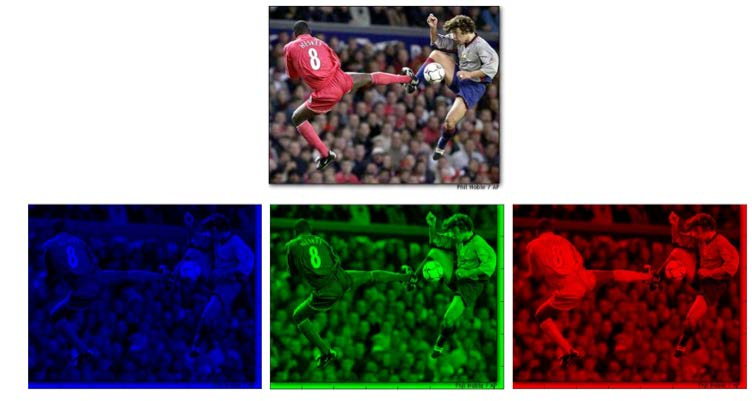
\includegraphics[width=\textwidth]{canali_rgb}
    \caption{Canali RGB di un'immagine}
  \end{minipage}
  \hfill
  \begin{minipage}[b]{0.46\textwidth}
    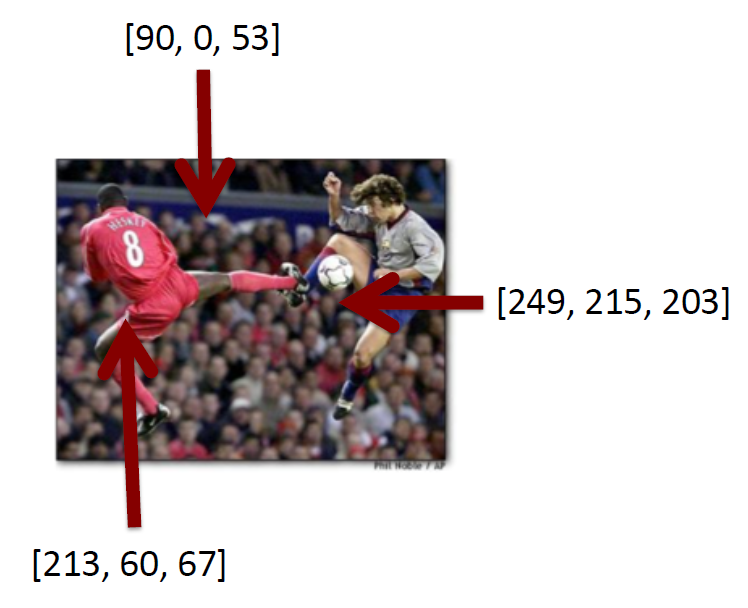
\includegraphics[width=\textwidth]{pixel}
    \caption{Pixel di un'immagine}
  \end{minipage}
\end{figure}

Si può immaginare il tensore immagine $\mathcal{I}$ come una "pila" di tre matrici, una per ogni canale di colore, come mostrato in figura \ref{rappresentazione_tensore}.

\begin{figure}
\centering
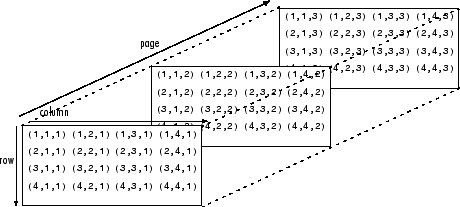
\includegraphics[scale=0.7]{rappresentazione_tensore}
\caption{Rappresentazione grafica di un tensore tridimensionale; in ogni posizione compaiono gli indici del tensore}
\label{rappresentazione_tensore}
\end{figure}

\subsection{Supervised Learning}

Il paradigma dell'\textbf{apprendimento supervisionato} (\textit{supervised learning})
consiste nel creare un algoritmo in grado di apprendere una funzione che mappi un input all'output corretto, sulla base di una serie di esempi ideali, costituiti da coppie di input e dei relativi output attesi, che gli vengono inizialmente forniti per addestrarlo \cite{Russell2009}.
Un algoritmo di apprendimento supervisionato analizza i dati di addestramento e inferisce una funzione che può essere usata per mappare nuovi input ai corretti output. Ciò richiede all'algoritmo la capacità di trovare una funzione che sappia generalizzare efficacemente dai dati di training, al fine di adattarsi bene a nuovi dati (per poterne mappare correttamente quanti più possibile).\\

Molti problemi pratici, come ad esempio la regressione e la classificazione, possono essere formulati ricorrendo ad una funzione matematica
\[\mathcal{F}:X\to Y\]
che associa ad ogni elemento nello spazio degli input $X$ (dataset) uno ed un solo elemento dello spazio degli output.
Il concetto di funzione implica l'esistenza di un solo elemento di $Y$ a cui ogni elemento di $X$ è correttamente associato. Il problema consiste allora nel cercare una funzione $\mathcal{F}$ in grado di ottenere esattamente tale associazione, per quanti più elementi di $X$ possibile.

È evidente che questo tipo di problemi ben si presta ad essere approcciato con algoritmi di apprendimento supervisionato.

Prima di analizzare in dettaglio il problema di classificazione delle immagini oggetto della presente tesi, è necessario inquadrare il problema partendo da alcune definizioni preliminari.\\

Un \textbf{dataset} X è una generica collezione di $N$ dati
\[X=\{\mathbf{x}^{(1)},\mathbf{x}^{(2)},\dots,\mathbf{x}^{(N)}\}\]
Ogni dato $\mathbf{x}^{(i)}$ è chiamato \textbf{esempio} (o \textbf{data point}).
I data point possono essere anche non omogenei tra loro (cioè avere dimensioni differenti).
Ciascun esempio si può caratterizzare come un vettore $\mathbf{x}^{(i)}\in\R^{D}$, in cui ciascun elemento $x_i$ è detto \textbf{feature} e rappresenta una caratteristica di un oggetto o un evento misurato. $D$ è il numero di feature in ogni esempio, o \textbf{dimensione} dell'esempio.
In caso di esempi omogenei (cioè aventi stessa dimensione $D$) un dataset può essere descritto attraverso una matrice detta \textbf{design matrix}, in cui ogni riga corrisponde ad un particolare esempio e ogni colonna corrisponde ad una precisa feature.
Un dataset di cardinalità $N$ e in cui ogni esempio ha $D$ feature ha quindi una design matrix di dimensione $N\times D$. \\

In un problema di classificazione delle immagini orientato all'\textit{object recognition} (riconoscimento di un oggetto in un immagine), sussiste la seguente caratterizzazione:
\begin{itemize}
\item $X$: un insieme di $N$ immagini digitali
\item $Y$: un insieme di $K$ classi predefinite di oggetti che possono essere individuati all'interno di un'immagine (possono essere dei "descrittori" testuali o, equivalentemente, dei numeri interi)
\end{itemize}
Un elemento di $Y$ è solitamente chiamato \textbf{etichetta} o \textbf{categoria} (in inglese \textbf{label} o \textbf{class}); si dice quindi che ogni immagine $\mathbf{x}^{(i)}\in X$ può essere \textit{descritta da un'etichetta} (o \textit{associata ad una categoria}) $\mathbf{y}^{(i)}\in Y$ tramite una funzione di associazione $f$.\footnote{Teoricamente una stessa immagine potrebbe essere descritta da più di un'etichetta o addirittura da nessuna, coerentemente col fatto che in essa potrebbero essere presenti più oggetti o nessun oggetto tra quelli previsti in $Y$. Tuttavia nella presente tesi questa ambiguità non può sussistere: la classificazione riduce qualsiasi immagine ad una di due categorie mutualmente esclusive e di cui almeno una deve essere ammessa, cioè la presenza o meno di una pinna nell'immagine.}\\
Nella pratica, TODO f non può essere trovata esattamente. (vd gianvito)

TODO: scrivere ora o in un paragrafo a parte i tipi di dato per gestire le immagini messi a disposizione da matlab.


\section{Classificatore lineare}
Il classificatore lineare è una tra le più semplici funzioni di classificazione.\footnote{La fonte principale per gli argomenti trattati in questo paragrafo è \cite{cs231n}}
Ipotizziamo di avere un insieme di $N$ immagini $\mathbf{x}^{(i)}$ (\textit{data points}), ciascuna con risoluzione fissa $w\times h$ e in formato RGB ($c=3$), e un insieme di $K$ distinte categorie di oggetti  (\textit{labels}). Un \textbf{classificatore lineare} è definito dalla funzione
\begin{equation} \label{eq_class_lin}
f(\mathbf{x}^{(i)};\mathbf{W},\mathbf{b})=\mathbf{W}\mathbf{x}^{(i)}+\mathbf{b}
\end{equation}
In questa espressione stiamo assumendo che $\mathbf{x}^{(i)}$ sia un vettore colonna di dimensione $D=hwc$ ottenuto incolonnando una ad una le righe dell'$i$-esima immagine di tutti e tre i canali di colore, $\mathbf{W}$ una matrice detta \textbf{matrice dei pesi} (\textit{weights matrix}) di dimensione $K\times D$ e $\mathbf{b}$ un vettore colonna detto \textbf{vettore dei bias} (\textit{bias vector}) di dimensione $K$. I pesi e i bias sono parametri della funzione $f$.

Ogni riga $j$-esima di $W$ e il relativo $j$-esimo valore di $\mathbf{b}$ serve a calcolare la combinazione (lineare a meno del bias) $\mathbf{w}_j\cdot \mathbf{x}^{(i)}+b_j$. Ognuna delle $K$ combinazioni calcolate è un numero reale che si può interpretare come un "punteggio" registrato dall'$i$-esima immagine in ogni classe di oggetti in $Y$ (\textit{class score}): l'$i$-esima immagine è classificata con l'etichetta $\mathbf{y}_j\in Y$ se l'elemento $j$-esimo del vettore output $f(\mathbf{x}^{(i)};\mathbf{W},\mathbf{b})$ è il massimo del medesimo vettore.\\

L'esempio in figura \ref{class_lin} mostra la classificazione di un'immagine di un gatto con $\abs{Y}=3$ classi (\textit{gatto}, \textit{cane}, \textit{barca}). Per semplicità, l'immagine input è ipotizzata $2\times 2$ e composta da un unico canale di colore ($c=1$) (quindi $\mathbf{x}$, scritta come vettore colonna, è $4\times 1$).

\begin{figure}[h]
\centering
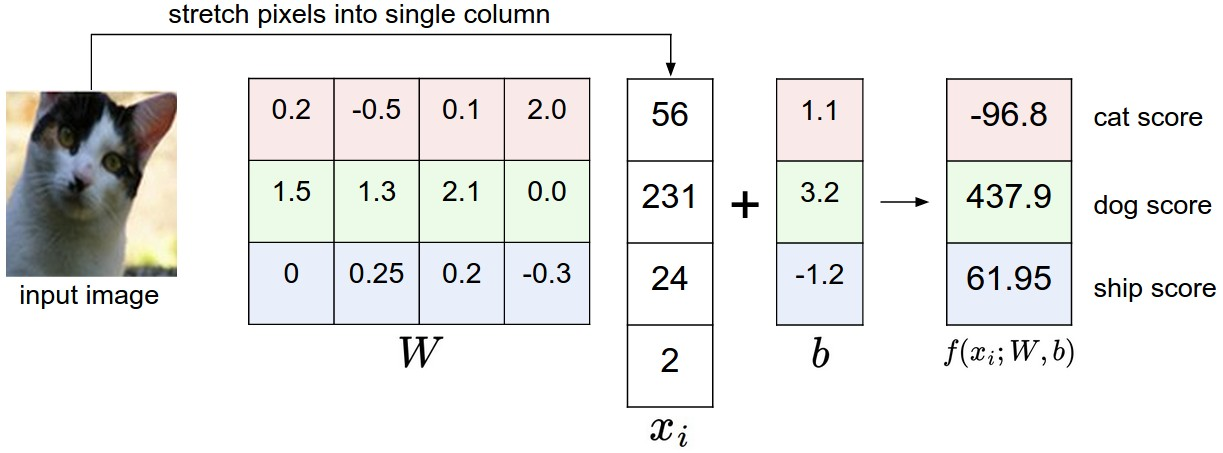
\includegraphics[width=\textwidth ,keepaspectratio]{classificatore_lineare}
\caption{Mappatura di un'immagine ai punteggi di ogni classe mediante un classificatore lineare. Si noti che i pesi di $\mathbf{W}$ non costituiscono un buon set di parametri: il punteggio assegnato alla classe "cane" (sbagliata) è alto e quello totalizzato dalla classe "gatto" (corretta) è basso. Il classificatore "è convinto" di aver classificato l'immagine di un cane.}
\label{class_lin}
\end{figure}

\subsection*{Interpretare un classificatore lineare}

Poiché le immagini possono essere memorizzate come vettori colonna $hwc$-dimensionali, si possono immaginare le immagini di un dataset come dei punti nello spazio $\R^{hwc}$. Di conseguenza, il dataset può essere pensato come una collezione di punti multidimensionali. Ovviamente non possiamo visualizzare spazi con più dimensioni di $\R^{3}$, ma se immaginiamo di "comprimere" tutte le $hwc$ dimensioni in sole due dimensioni otteniamo una visualizzazione del tipo in figura \ref{visual_class_lin}.

\begin{figure}[h]
\centering
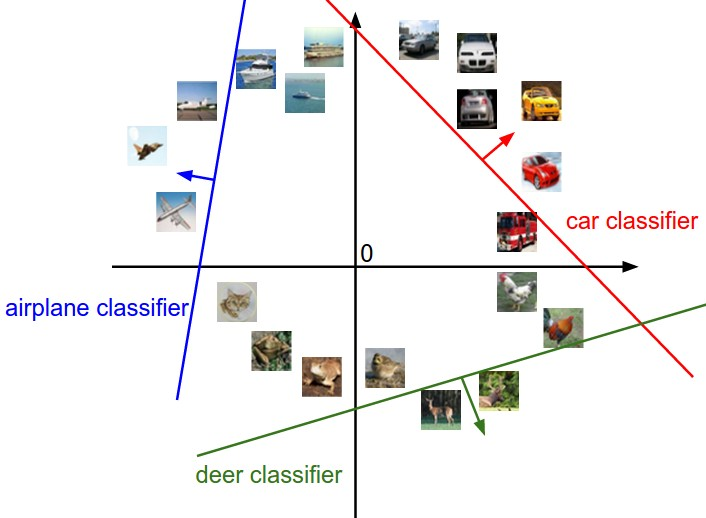
\includegraphics[width=\textwidth ,keepaspectratio]{visualizz_class_lin}
\caption{Visualizzazione di tre righe di un classificatore lineare, una per ciascuna delle classi "aereo", "auto", "cervo".}
\label{visual_class_lin}
\end{figure}

Le rette in figura devono in realtà essere pensate come degli iperpiani $(hwc-1)$-dimensionali, associati a ciascuna classe di $Y$ (cioè a ciascuna riga di $\mathbf{W}$ e $\mathbf{b}$), e il piano come lo spazio $\R^{hwc}$. Sussistono le seguenti interpretazioni geometriche:
\begin{itemize}
\item Le immagini sono dei punti nel piano. Ogni retta è il luogo dei punti che totalizzano un punteggio nullo per la classe associata a quella retta (la classe è scritta in figura accanto ad ogni retta). La freccia nella figura indica la direzione seguendo la quale i punti del piano aumentano (linearmente) il punteggio realizzato per quella classe.
\item Modificare i pesi di $\mathbf{W}$ significa regolare l'inclinazione delle rette (cioè ruotarle rispetto al punto di intercetta).
\item Modificare i bias di $\mathbf{b}$ significa regolare l'intercetta delle rette (cioè traslarle verticalmente).
\end{itemize}

Un altro modo di interpretare i pesi $\mathbf{W}$ può essere quello di far corrispondere ogni riga di $\mathbf{W}$ a un \textbf{prototipo} (in inglese \textbf{template}) per una delle classi. In questa interpretazione, il punteggio realizzato per ogni classe da un'immagine è ottenuto attraverso l'operazione di prodotto matriciale tra il prototipo della classe $j$ ($\mathbf{w}_j$) e l'immagine da classificare ($\mathbf{x}^{(i)}$).
Usando la terminologia introdotta, possiamo affermare che ciò che sta facendo il classificatore lineare è un'operazione di \textit{template matching}, dove i \textit{templates} sono oggetto di apprendimento da parte del classificatore\footnote{Si introdurranno gli algoritmi di apprendimento (supervisionato) nel capitolo \ref{TODO}.}.

Ad esempio, analizziamo il dataset \textit{CIFAR-10} \cite{cifar10}. Esso contiene immagini $32\times 32$ ciascuna appartenente ad una di 10 classi. Visualizzando\footnote{TODO Per i dettagli su come "visualizzare" i pesi si veda \url{https://it.mathworks.com/help/deeplearning/examples/visualize-activations-of-a-convolutional-neural-network.html}.} i pesi (e quindi i 10 templates) di un classificatore lineare addestrato su CIFAR-10 si ottengono i risultati in figura seguente:

\begin{figure}[h]
\centering
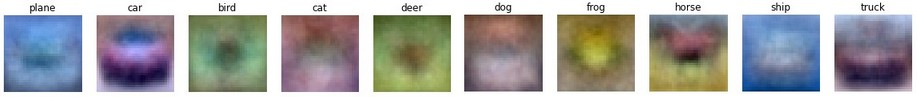
\includegraphics[width=\textwidth ,keepaspectratio]{templates}
\caption{Visualizzazione dei templates di un classificatore addestrato sul dataset CIFAR-10}
\label{templates}
\end{figure}

Si possono fare alcune interessanti osservazioni.

Ad esempio, il prototipo della classe "barca" è composto da molti pixel blu disposti perlopiù lungo i margini, come ci si potrebbe aspettare dal momento che molte immagini di barche in CIFAR-10 raffigurano queste in mare aperto. Questo template allora assegnerà un punteggio alto quando l'immagine che si vuole classificare (cioè \textit{raffrontare al template}) è una barca in mare aperto. In altre parole, un'immagine realizzerà un punteggio tanto più alto in una certa classe quanto più essa è \textit{simile} al template che il classificatore lineare \textit{ha imparato} per quella classe.

Il prototipo per la classe "cavallo" sembra essere l'immagine di un cavallo a due teste; similmente, quello per la classe "auto" sembra una miscela di rappresentazioni di un'auto vista da più direzioni diverse. Ciò è coerente col fatto che il classificatore lineare è stato addestrato su immagini di cavalli visti rispetto a entrambi i profili e su immagini
di auto raffigurate in tante direzioni diverse. Inoltre, il template per l'auto sembra rappresentare un'auto di colore rosso: evidentemente in CIFAR-10 la maggior parte delle automobili rappresentate sono di quel colore.\\

Come si vedrà nel seguito, questa operazione di \textit{template matching} presenta una forte analogia con il funzionamento di un \textit{Fully Connected Layer} di una rete neurale convoluzionale.

\subsection*{Bias trick}
Concludiamo questo capitolo menzionando un "trucco" matematico molto utilizzato per rappresentare $\mathbf{W}$ e $\mathbf{b}$ come un'unica matrice, semplificando la notazione \ref{eq_class_lin}.
Possiamo aggiungere il vettore dei bias in coda alla matrice dei pesi e aggiungere un "1" in coda al vettore che rappresenta l'immagine. In questo modo, il classificatore lineare è rappresentato dalla funzione di associazione
\begin{equation} \label{eq_bias_trick}
f(\mathbf{x}^{(i)};\mathbf{W})=\mathbf{W}\mathbf{x}^{(i)}
\end{equation}

In questa maniera, $f$ calcola solo combinazioni lineari (un singolo prodotto matriciale), poiché il vettore dei bias è stato eliminato.
Tale utile passaggio, noto come \textit{bias trick}, è visualizzato nella seguente figura

\begin{figure}[h]
\centering
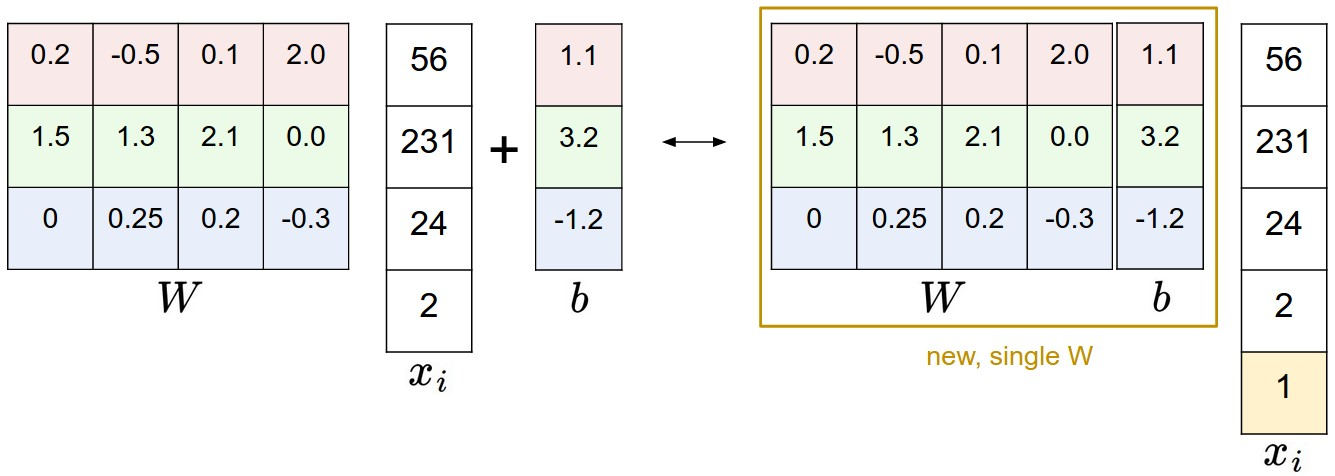
\includegraphics[width=\textwidth ,keepaspectratio]{bias_trick}
\caption{Bias trick}
\label{bias_trick}
\end{figure}

TODO: loss functions.
\subsection{Machine Learning e Deep Learning}
Il \textit{machine learning} è una branca dell'intelligenza artificiale (AI) che si occupa in generale di fornire ad una macchina la capacità di apprendere automaticamente dall'esperienza, essendo esplicitamente programmata su "come imparare" ma non su "cosa imparare".

Questa capacità è fornita da un algoritmo di machine learning, di cui T. Mitchell fornisce una celebre ed elegante definizione:
\begin{quote}
Si dice che un programma per computer impara dall’esperienza E rispetto ad una qualche classe di compiti T ed una misura di performance P se le sue prestazioni nei compiti in T, misurate attraverso P, migliorano con l’esperienza E.
\end{quote}

L'obiettivo principale dell'apprendimento automatico è che una macchina sia in grado di generalizzare dalla propria esperienza\cite{bishop}, ossia che sia in grado di svolgere ragionamenti induttivi. In questo contesto, per generalizzazione si intende l'abilità di una macchina di portare a termine in maniera accurata esempi o compiti nuovi, che non ha mai affrontato, dopo aver fatto esperienza su un insieme di dati di apprendimento.
Gli esempi di addestramento (in inglese chiamati \textit{training examples}) si assume provengano da una qualche distribuzione di probabilità, generalmente sconosciuta e considerata rappresentativa dello spazio delle occorrenze del fenomeno da apprendere; la macchina ha il compito di costruire un modello probabilistico generale dello spazio delle occorrenze, in maniera tale da essere in grado di produrre previsioni sufficientemente accurate quando sottoposta a nuovi casi.

Quasi tutti gli algoritmi di machine learning sono costruiti combinando almeno quattro
building blocks fondamentali: un dataset, un modello, una funzione costo ed un
metodo di ottimizzazione.\\

Il \textit{deep learning} è un tipo specifico di machine learning, che negli ultimi anni ha dato una svolta decisiva alla più vasta branca dell’intelligenza artificiale.

Un algoritmo di deep learning si basa su diversi livelli di rappresentazione dei dati, che corrispondono a differenti livelli di astrazione; questi livelli formano una gerarchia di concetti, in cui i concetti di più alto livello sono definiti sulla base di quelli di livello più basso.

Il modello computazionale utilizzato in maniera esclusiva nel \textit{deep learning} è la rete neurale artificiale (par. \ref{ANN})\\

Il deep learning è inquadrato in una più ampia branca del machine learning, chiamata \textbf{\textit{representation learning}}. Nell'ambito del representation learning, l'approccio usato per la risoluzione dei problemi consiste non solo nel tentare di addestrare un computer a trovare una relazione tra dati e output, ma anche nel fornirgli strumenti per la rappresentazione stessa dei dati, in quanto in alcuni contesti il legame tra i dati in input e quelli attesi in output è tutt'altro che lineare ed è in generale complesso, e può essere più facile per la macchina acquisire diversi livelli di conoscenza e di astrazione dei dati in input per calcolare l'output.

Si pensi ad esempio ad un task di \textit{image classification}. È impensabile descivere la presenza di un oggetto all’interno di un'immagine attraverso un legame lineare con i singoli pixel. È piuttosto la combinazione di pixel l'informazione da mappare (in maniera in generale non lineare) con la categoria di appartenenza di quell'oggetto.

Dagli studi scientifici sull'apparato visivo sappiamo che l'uomo riesce a riconoscere gli oggetti attraverso una rappresentazione gerarchica degli stessi:

\begin{itemize}
\item dapprima captiamo caratteristiche di basso livello degli oggetti che vediamo, come forme (spigoli, angoli) e tonalità di colore. Tutte queste caratteristiche sono "locali", nel senso che occupano una regione limitata del campo visivo, essendo parti più piccole dell'oggetto. In questa fase, non sappiamo ancora dare un nome all'oggetto su cui ci concentriamo;
\item queste caratteristiche (\textit{features}) sono combinate nella parte del cervello che si occupa della visione, a formare concetti di più alto livello come il perimetro dell'oggetto e le sfumature (gradienti) di colore;
\item questa rappresentazione graduale e gerarchica dei concetti, arrivata a concetti di più alto livello, permette infine di associare alla "immagine" formatasi nel nostro campo visivo il nome dell'oggetto, o degli oggetti, in esso presenti.
\end{itemize}

Sulle medesime basi "biologiche" si fondano le reti neurali artificiali, attraverso gli \textit{hidden layers} (strati nascosti) frapposti tra l'input e l'output della rete stessa che permettono di combinare le informazioni provenienti dagli strati precedenti per ottenere una rappresentazione dei dati di più alto livello.

\begin{figure}[h]
\centering
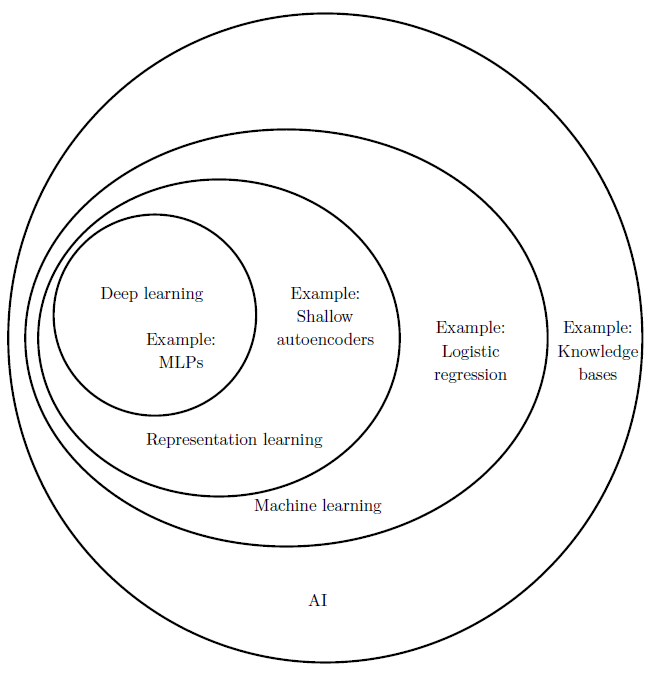
\includegraphics[width=0.7\textwidth]{diagrammaIA}
\caption{Un diagramma di Venn che mostra come il deep learning sia un tipo di
representation learning, che a sua volta è un tipo di machine learning.}
\label{diagrammaAI}
\end{figure}


\subsection{Supervised Learning}
\label{supervisedLearning}

Il paradigma dell'\textbf{apprendimento supervisionato} (\textit{supervised learning}) mira alla creazione di un algoritmo che analizzi dei "dati di addestramento", una collezione di esempi ideali costituiti da coppie di input e relativi output attesi, e da questi inferisca una funzione che può essere usata per mappare nuovi input ai corretti output \cite{Russell2009}.
Ciò richiede all'algoritmo la capacità di trovare una funzione che sappia generalizzare efficacemente dai dati di training, al fine di adattarsi bene a nuovi dati (per poterne mappare correttamente quanti più possibile).\\

Molti problemi pratici, come ad esempio la regressione e la classificazione delle immagini (par. \ref{objectRecognition}, possono essere formulati ricorrendo ad una funzione matematica
\[\mathcal{F}:X\to Y\]
che associa ad ogni elemento dello spazio degli input $X$ uno ed un solo elemento dello spazio degli output $Y$.
Il concetto di funzione implica l'esistenza di un solo elemento di $Y$ a cui ogni elemento di $X$ è correttamente associato. Il problema consiste allora nel cercare una funzione $\mathcal{F}$ in grado di ottenere esattamente tale associazione, per quanti più elementi di $X$ possibile.

È evidente che questo tipo di problemi ben si presta ad essere approcciato con algoritmi di apprendimento supervisionato.

Prima di analizzare in dettaglio il problema di classificazione delle immagini oggetto della presente tesi, è necessario inquadrare il problema partendo da alcune definizioni preliminari.\\

Un \textbf{dataset} X è una generica collezione di $N$ dati
\[X=\{\mathbf{x}^{(1)},\mathbf{x}^{(2)},\dots,\mathbf{x}^{(N)}\}\]
Ogni dato $\mathbf{x}^{(i)}$ è chiamato \textbf{esempio} (o \textbf{data point}).
I data point possono essere anche non omogenei tra loro (cioè avere dimensioni differenti).
Ciascun esempio si può caratterizzare come un vettore $\mathbf{x}^{(i)}\in\R^{D}$, in cui ciascun elemento $x_i$ è detto \textbf{feature} e rappresenta una caratteristica di un oggetto o un evento misurato. $D$ è il numero di feature in ogni esempio, o \textbf{dimensione} dell'esempio.
In caso di esempi omogenei (cioè aventi stessa dimensione $D$) un dataset può essere descritto attraverso una matrice detta \textbf{design matrix}, in cui ogni riga corrisponde ad un particolare esempio e ogni colonna corrisponde ad una precisa feature.
Un dataset di cardinalità $N$ e in cui ogni esempio ha $D$ feature ha quindi una design matrix di dimensione $N\times D$. \\

In un problema di classificazione delle immagini sussiste la seguente caratterizzazione:
\begin{itemize}
\item $X$: un insieme di $N$ immagini digitali
\item $Y$: un insieme di $K$ classi predefinite di oggetti che possono essere individuati all'interno di un'immagine (possono essere dei "descrittori" testuali o, equivalentemente, dei numeri interi)
\end{itemize}
Un elemento di $Y$ è solitamente chiamato \textbf{etichetta} o \textbf{categoria} (in inglese \textbf{label} o \textbf{class}); si dice quindi che ogni immagine $\mathbf{x}^{(i)}\in X$ può essere \textit{descritta da un'etichetta} (o \textit{associata ad una categoria}) $\mathbf{y}^{(i)}\in Y$ tramite una funzione di associazione $f$.\footnote{Teoricamente una stessa immagine potrebbe essere descritta da più di un'etichetta o addirittura da nessuna, coerentemente col fatto che in essa potrebbero essere presenti più oggetti o nessun oggetto tra quelli previsti in $Y$. Tuttavia nella presente tesi questa ambiguità non può sussistere: la classificazione riduce qualsiasi immagine ad una di due categorie mutualmente esclusive e di cui soltanto una è quella corretta, cioè la presenza o meno di una pinna nell'immagine.}\\

Tipicamente, per l'addestramento di un modello di machine learning si usa un sottoinsieme del dataset $X$ a disposizione. Questo sottoinsieme $X^{train}$ è definito \textbf{\textit{training set}}.

Nella pratica, l'espressione analitica di $f$ non può essere trovata esattamente. Ad esempio, nel problema in esame, non è chiaro come poter scrivere un algoritmo che consenta di individuare con esattezza la presenza di una pinna all'interno di un'immagine, poiché il concetto di "pinna" non è un concetto matematico e non può essere reso facilmente in un linguaggio "comprensibile" da un computer. Inoltre, il computer può disporre solamente di un numero limitato $\left|X^{(train)}\right|$ di esempi, cioè un numero limitato di occorrenze di oggetti di tipo "pinna", che non permettono di generalizzare a tutte le forme ed i colori in cui una pinna può essere presente in un'immagine. Per questo motivo, ciò che il modello di machine learning da addestrare è chiamato ad imparare è un'approssimazione quanto più "plausibile" di $f$, dove per "plausibilità" si intende la capacità della funzione trovata di restituire il giusto output per il maggior numero possibile di input presentati.

\subsection{Underfitting e overfitting}
\label{overfitting}
La sfida principale dell'apprendimento automatico è quella di rendere l'algoritmo di machine learning performante su nuovi input, diversi da quelli su cui il modello è stato addestrato. Questa abilità è chiamata \textbf{generalizzazione}.\\

Tipicamente, dopo l'addestramento di un modello di machine learning con un \textit{training set} possiamo misurare le performance del modello con un parametro detto \textit{training error}, definito come il rapporto tra il numero di esempi del dataset che alla fine dell'addestramento l'algoritmo associa al giusto output, $\left|X_{corrette}\right|<\left|X\right|$, e la dimensione del \textit{training set}, $\left|X\right|$:
\[\text{Training Error}=\frac{\left|X_{corrette}\right|}{\left|X\right|}\]
Ovviamente, con l'addestramento si vuole minimizzare questo rapporto. Quello descritto è un problema di ottimizzazione.\\

Tuttavia non basta che il modello si comporti bene su una collezione di dati di cui fondamentalmente si conosceva già l'output (abilità di per sé abbastanza inutile), ma si vuole, come già spiegato, che esso lavori bene anche su un \textbf{test set} $T$ di esempi mai forniti in input per l'addestramento del modello, e pertanto non presenti nel training set. Si può definire similmente al \textit{training error} un parametro detto \textbf{\textit{generalization error}} (errore di generalizzazione), o \textbf{\textit{test error}}.
\[\text{Test Error}=\frac{|T_{corrette}|}{|T|}\]
Si vuole ovviamente che anche il test error, come il training error, sia piccolo. Più precisamente, si vuole che la differenza tra il training error e il test error sia quanto più piccola possibile.\footnote{Il problema di ottimizzazione da risolvere è quello della minimizzazione del training error. Il test error non può essere minimizzato, in quanto esso viene valutato quando l'addestramento della rete è finito; anche in fase di training, comunque, il test set non è disponibile per l'addestramento (non può essere trattato come un'estensione del training set, pena la violazione della definizione stessa di "test set").}\\

I fattori che determinano quanto bene un algoritmo di machine learning performerà sono in definitiva le sue capacità di
\begin{enumerate}
\item rendere piccolo il training error
\item rendere piccola la differenza tra training error e test error
\end{enumerate}

Quando un modello non riesce ad ottenere un errore sufficientemente basso sul training set si dice che il modello soffre di \textbf{\textit{underfitting}} (sottoadattamento). Quando il modello non riesce a rendere piccola a sufficienza la differenza tra training error e test error si dice che il modello soffre di \textbf{\textit{overfitting}} (sovradattamento).

Possiamo controllare la tendenza di un modello all'underfitting o all'overfitting  regolando la sua \textbf{capacità}. Informalmente, la capacità di un modello è la sua abilità ad adattarsi ad un insieme ampio di funzioni. Modelli con capacità bassa potrebbero avere difficoltà nell'adattarsi al training set (underfitting). Al contrario, modelli con capacità alta hanno una maggiore probabilità di adattarsi troppo bene al training set (overfitting), memorizzando molte caratteristiche e proprietà degli esempi del training set che non sempre aiutano nella generalizzazione ai nuovi casi, ad esempio quelli del test set.

In una rete neurale (par. \ref{ANN}) la capacità del modello può essere definita, ad esempio, come il numero di parametri addestrabili (pesi e bias) che la caratterizzano.

Gli algoritmi di machine learning performeranno generalmente bene quando la loro capacità è appropriata rispetto alla reale complessità del task che devono svolgere e alla quantità di esempi $|X^{train}|$ forniti per l'addestramento. Modelli con una capacità insufficiente non riescono a risolvere task complessi. Modelli con alta capacità possono risolvere task complessi, ma se la loro capacità è eccessivamente alta rispetto alla complessità del task in esame potrebbero soffire di overfitting. La fig. \ref{fig:capacity} presenta bene la situazione.

\begin{figure}[h]
\centering
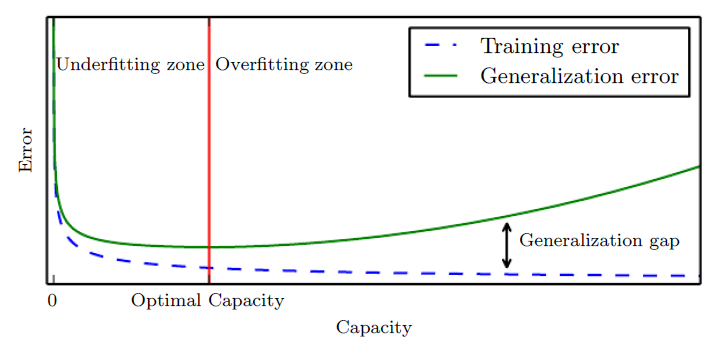
\includegraphics[width=0.8\textwidth]{capacity}
\caption{Training error e test error (asse y) al variare della capacità del modello (asse x)}
\label{fig:capacity}
\end{figure}

Negli esperimenti condotti una delle reti neurali utilizzate (ResNet-50) ha sofferto di overfitting a causa della sua enorme capacità di rappresentazione e del training set relativamente ristretto usato per il suo addestramento (par. \ref{addestramento}).

\section{Classificazione}
In un problema di classificazione l’insieme delle classi $Y$ è discreto e finito.
Sulla base del numero di classi $|Y|$ si distinguono due tipi di classificazione: binaria ($|Y|=2$) o multiclasse ($|Y|>2$).

TODO magari lo inserisco direttamente nel capitolo sulle reti neurali.








\section{Classificatore lineare}
Il classificatore lineare è uno tra i più semplici modelli di classificazione.
Ipotizziamo di avere un insieme di $N$ immagini $\mathbf{x}^{(i)}$ (\textit{data points}), ciascuna con risoluzione fissa $w\times h$ e in formato RGB ($c=3$), e un insieme di $K$ distinte categorie di oggetti  (\textit{labels}). Un \textbf{classificatore lineare} è definito dalla funzione
\begin{equation} \label{eq_class_lin}
f(\mathbf{x}^{(i)};\mathbf{W},\mathbf{b})=\mathbf{W}\mathbf{x}^{(i)}+\mathbf{b}
\end{equation}
In questa espressione stiamo assumendo che $\mathbf{x}^{(i)}$ sia un vettore colonna di dimensione $D=hwc$ ottenuto incolonnando una ad una le righe dell'$i$-esima immagine di tutti e tre i canali di colore, $\mathbf{W}$ una matrice detta \textbf{matrice dei pesi} (\textit{weights matrix}) di dimensione $K\times D$ e $\mathbf{b}$ un vettore colonna detto \textbf{vettore dei bias} (\textit{bias vector}) di dimensione $K$. I pesi e i bias sono parametri della funzione $f$.

Ogni riga $j$-esima di $W$ e il relativo $j$-esimo valore di $\mathbf{b}$ serve a calcolare la combinazione (lineare a meno del bias) $\mathbf{w}_j\cdot \mathbf{x}^{(i)}+b_j$. Ognuna delle $K$ combinazioni calcolate è un numero reale che si può interpretare come un "punteggio" registrato dall'$i$-esima immagine in ogni classe di oggetti in $Y$ (\textit{class score}): l'$i$-esima immagine è classificata con l'etichetta $\mathbf{y}_j\in Y$ se l'elemento $j$-esimo del vettore output $f(\mathbf{x}^{(i)};\mathbf{W},\mathbf{b})$ è il massimo del medesimo vettore.\\

L'esempio in figura \ref{class_lin} mostra la classificazione di un'immagine di un gatto con $\abs{Y}=3$ classi (\textit{gatto}, \textit{cane}, \textit{barca}). Per semplicità, l'immagine input è ipotizzata $2\times 2$ e composta da un unico canale di colore ($c=1$) (quindi $\mathbf{x}$, scritta come vettore colonna, è $4\times 1$).

\begin{figure}[h]
\centering
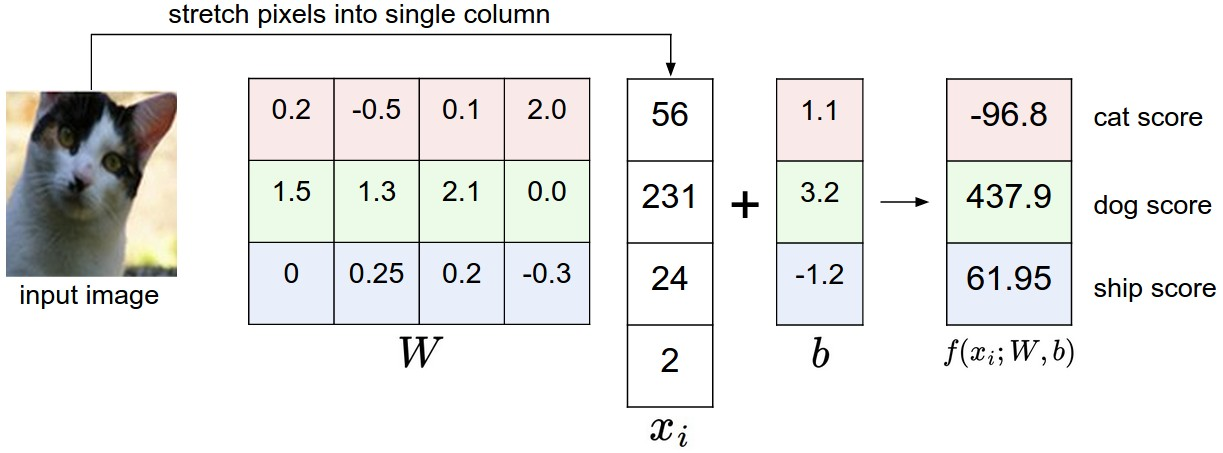
\includegraphics[width=\textwidth ,keepaspectratio]{classificatore_lineare}
\caption{Mappatura di un'immagine ai punteggi di ogni classe mediante un classificatore lineare. Si noti che i pesi di $\mathbf{W}$ non costituiscono un buon set di parametri: il punteggio assegnato alla classe "cane" (sbagliata) è alto e quello totalizzato dalla classe "gatto" (corretta) è basso. Il classificatore "è convinto" di aver classificato l'immagine di un cane.}
\label{class_lin}
\end{figure}

\subsection*{Interpretare un classificatore lineare}

Poiché le immagini possono essere memorizzate come vettori colonna $hwc$-dimensionali, si possono immaginare le immagini di un dataset come dei punti nello spazio $\R^{hwc}$. Di conseguenza, il dataset può essere pensato come una collezione di punti multidimensionali. Ovviamente non possiamo visualizzare spazi con più dimensioni di $\R^{3}$, ma se immaginiamo di "comprimere" tutte le $hwc$ dimensioni in sole due dimensioni otteniamo una visualizzazione del tipo in figura \ref{visual_class_lin}.

\begin{figure}[h]
\centering
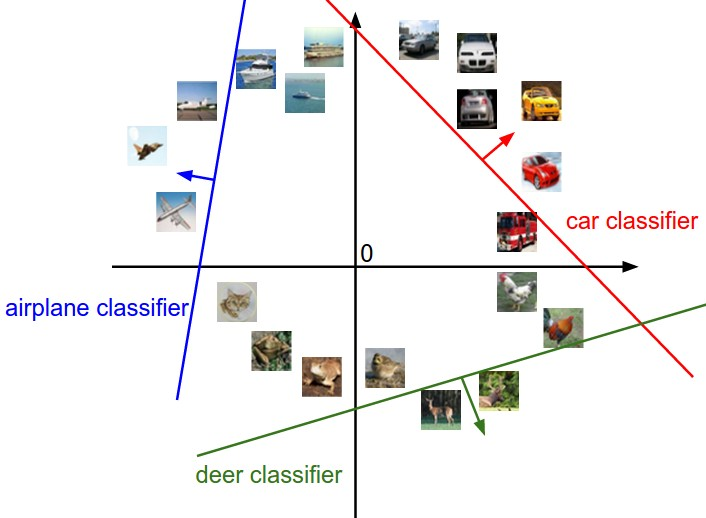
\includegraphics[width=\textwidth ,keepaspectratio]{visualizz_class_lin}
\caption{Visualizzazione di tre righe di un classificatore lineare, una per ciascuna delle classi "aereo", "auto", "cervo".}
\label{visual_class_lin}
\end{figure}

Le rette in figura devono in realtà essere pensate come degli iperpiani $(hwc-1)$-dimensionali, associati a ciascuna classe di $Y$ (cioè a ciascuna riga di $\mathbf{W}$ e $\mathbf{b}$), e il piano come lo spazio $\R^{hwc}$. Sussistono le seguenti interpretazioni geometriche:
\begin{itemize}
\item Le immagini sono dei punti nel piano. Ogni retta è il luogo dei punti che totalizzano un punteggio nullo per la classe associata a quella retta (la classe è scritta in figura accanto ad ogni retta). La freccia nella figura indica la direzione seguendo la quale i punti del piano aumentano (linearmente) il punteggio realizzato per quella classe.
\item Modificare i pesi di $\mathbf{W}$ significa regolare l'inclinazione delle rette (cioè ruotarle rispetto al punto di intercetta).
\item Modificare i bias di $\mathbf{b}$ significa regolare l'intercetta delle rette (cioè traslarle verticalmente).
\end{itemize}

Un altro modo di interpretare i pesi $\mathbf{W}$ può essere quello di far corrispondere ogni riga di $\mathbf{W}$ a un \textbf{prototipo} (in inglese \textbf{template}) per una delle classi. In questa interpretazione, il punteggio realizzato per ogni classe da un'immagine è ottenuto attraverso l'operazione di prodotto matriciale tra il prototipo della classe $j$ ($\mathbf{w}_j$) e l'immagine da classificare ($\mathbf{x}^{(i)}$).
Usando la terminologia introdotta, possiamo affermare che ciò che sta facendo il classificatore lineare è un'operazione di \textit{template matching}, dove i \textit{templates} sono oggetto di apprendimento da parte del classificatore\footnote{Si introdurranno gli algoritmi di apprendimento (supervisionato) nel capitolo \ref{TODO}.}.

Ad esempio, analizziamo il dataset \textit{CIFAR-10} \cite{cifar10}. Esso contiene immagini $32\times 32$ ciascuna appartenente ad una di 10 classi. Visualizzando\footnote{TODO Per i dettagli su come "visualizzare" i pesi si veda \url{https://it.mathworks.com/help/deeplearning/examples/visualize-activations-of-a-convolutional-neural-network.html}.} i pesi (e quindi i 10 templates) di un classificatore lineare addestrato su CIFAR-10 si ottengono i risultati in figura seguente:

\begin{figure}[h]
\centering
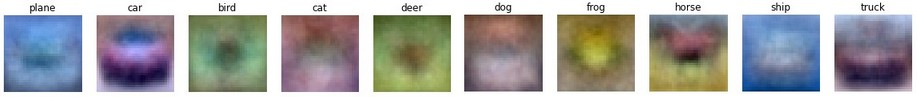
\includegraphics[width=\textwidth ,keepaspectratio]{templates}
\caption{Visualizzazione dei templates di un classificatore addestrato sul dataset CIFAR-10}
\label{templates}
\end{figure}

Si possono fare alcune interessanti osservazioni.

Ad esempio, il prototipo della classe "barca" è composto da molti pixel blu disposti perlopiù lungo i margini, come ci si potrebbe aspettare dal momento che molte immagini di barche in CIFAR-10 raffigurano queste in mare aperto. Questo template allora assegnerà un punteggio alto quando l'immagine che si vuole classificare (cioè \textit{raffrontare al template}) è una barca in mare aperto. In altre parole, un'immagine realizzerà un punteggio tanto più alto in una certa classe quanto più essa è \textit{simile} al template che il classificatore lineare \textit{ha imparato} per quella classe.

Il prototipo per la classe "cavallo" sembra essere l'immagine di un cavallo a due teste; similmente, quello per la classe "auto" sembra una miscela di rappresentazioni di un'auto vista da più direzioni diverse. Ciò è coerente col fatto che il classificatore lineare è stato addestrato su immagini di cavalli visti rispetto a entrambi i profili e su immagini
di auto raffigurate in tante direzioni diverse. Inoltre, il template per l'auto sembra rappresentare un'auto di colore rosso: evidentemente in CIFAR-10 la maggior parte delle automobili rappresentate sono di quel colore.\\

Come si vedrà nel seguito, questa operazione di \textit{template matching} presenta una forte analogia con il funzionamento di un \textit{Fully Connected Layer} di una rete neurale convoluzionale.

\subsection*{Bias trick}
Concludiamo questo capitolo menzionando un "trucco" matematico molto utilizzato per rappresentare $\mathbf{W}$ e $\mathbf{b}$ come un'unica matrice, semplificando la notazione \ref{eq_class_lin}.
Possiamo aggiungere il vettore dei bias in coda alla matrice dei pesi e aggiungere un "1" in coda al vettore che rappresenta l'immagine. In questo modo, il classificatore lineare è rappresentato dalla funzione di associazione
\begin{equation} \label{eq_bias_trick}
f(\mathbf{x}^{(i)};\mathbf{W})=\mathbf{W}\mathbf{x}^{(i)}
\end{equation}

In questa maniera, $f$ calcola solo combinazioni lineari (un singolo prodotto matriciale), poiché il vettore dei bias è stato eliminato.
Tale utile passaggio, noto come \textit{bias trick}, è visualizzato nella seguente figura

\begin{figure}[h]
\centering
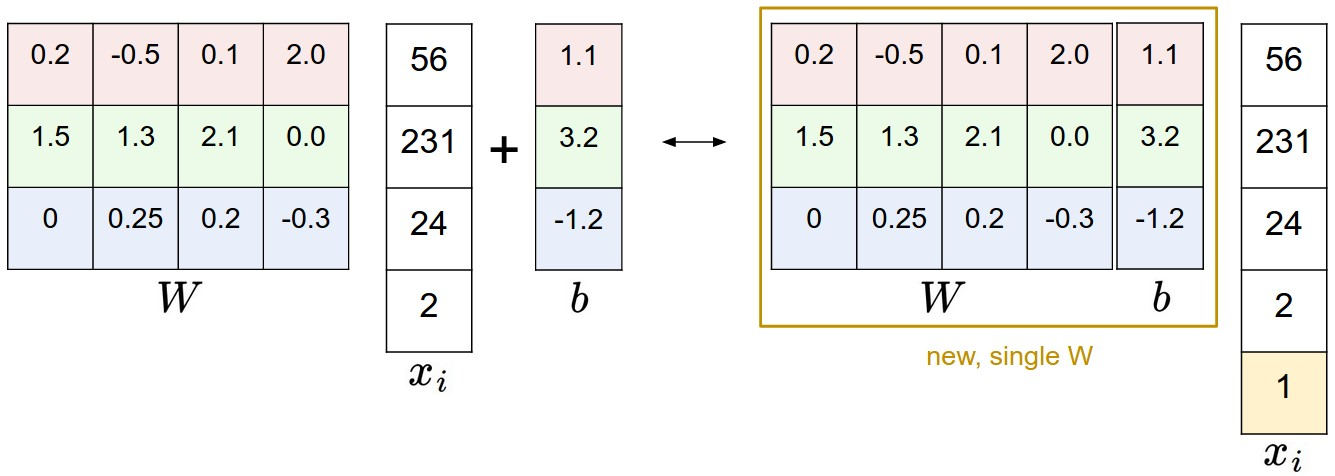
\includegraphics[width=\textwidth ,keepaspectratio]{bias_trick}
\caption{Bias trick}
\label{bias_trick}
\end{figure}

TODO: loss functions.

TODO: valutazione delle prestazioni di una rete neurale (matrice di confusione)



\section{Reti Neurali}
\label{ANN}

Le reti neurali artificiali (ANN, \textit{artificial neural networks}), costituiscono i modelli di deep learning per eccellenza.

Una rete neurale può essere interpretata come un insieme di strati (\textbf{\textit{layer}}) composti ciascuno da un certo numero di unità computazionali, dette \textbf{neuroni}, che nell'insieme sono in grado di fornire una nuova rappresentazione dell'input, secondo il paradigma del \textit{representation learning}. Le funzioni sono composte a formare una catena di rappresentazioni sconosciute (per questo dette \textit{hidden layers}), nel senso che ciascun layer calcola una funzione dell'output del layer precedente: a partire da rappresentazioni più semplici, esse vengono raggruppate fino ad un livello di arbitraria complessità
\begin{equation*}
\mathcal{F}(\mathbf{x})=\mathbf{f}^{(d)}\underbrace{(\dots(\mathbf{h}^{(3)}(\mathbf{h}^{(2)}(\mathbf{h}^{(1)}(\mathbf{x})))))}_{\text{hidden layers}}
\end{equation*}
in cui
\begin{itemize}
\item $d$ è la profondità della rete, cioè il numero di layers che la compongono;
\item $\mathbf{h}^{(1)}$ è il primo (hidden) layer, $\mathbf{h}^{(2)}$ il secondo, e così via. Ciascuno di essi rappresenta una trasformazione parametrica in generale non lineare delle feature relative ad un input $\mathbf{x}$: ogni hidden layer $\mathbf{h}$ accetta un vettore in input $\mathbf{x}$, calcola una
trasformazione affine $\mathbf{z}=\mathbf{W}\mathbf{x}+\mathbf{b}$, quindi applica una funzione non lineare $g(\mathbf{z})$
elemento per elemento, detta \textbf{funzione di attivazione}. Si ottiene così:
\begin{align*}
\text{Layer 1: } & \hspace{8mm}\mathbf{h}^{(1)}=g^{(1)}\left(\mathbf{W}^{(1)}\mathbf{x}+\mathbf{b}^{(1)}\right)\\
\text{Layer 2: } & \hspace{8mm}\mathbf{h}^{(2)}=g^{(2)}\left(\mathbf{W}^{(2)}\mathbf{h}^{(1)}+\mathbf{b}^{(2)}\right)\\
\text{Layer 3: } & \hspace{8mm}\mathbf{h}^{(3)}=g^{(3)}\left(\mathbf{W}^{(3)}\mathbf{h}^{(2)}+\mathbf{b}^{(3)}\right)
\end{align*}
fino a giungere all'output layer:
\begin{align*}
\text{Layer d: } & \hspace{8mm}\mathbf{f}^{(d)}=g^{(d)}\left(\mathbf{W}^{(d)}\mathbf{h}^{(d-1)}+\mathbf{b}^{(d)}\right)
\end{align*}
\item $f^{(d)}$ è l'output layer, che ha il ruolo di fornire un'ultima trasformazione al fine di completare il task che la rete deve eseguire. Le scelte solitamente sono:
\begin{itemize}
\item Layer di output lineare: viene calcolata una ulteriore trasformazione affine, del tipo
\begin{equation*}
\mathbf{\widehat{y}}=\mathbf{W}\mathbf{h}^{(d-1)}+\mathbf{b}
\end{equation*}
\item Layer di output softmax: viene calcolata una trasformazione affine
\begin{equation*}
\mathbf{z}=\mathbf{W}\mathbf{h}^{(d-1)}+\mathbf{b}
\end{equation*}
e viene quindi applicata la \textbf{funzione softmax}
\begin{equation*}
\mathbf{\widehat{y}}=\text{softmax}(\mathbf{z})_i=\frac{e^{z_i}}{\sum\nolimits_{j}e^{z_j}}
\end{equation*}
Grazie alla funzione softmax, l'output $\mathbf{\widehat{y}}$ è la distribuzione di probabilità che $\mathbf{x}$ appartenga alla classe $i$:
\begin{equation*}
\widehat{y_i}=p(y=i|\mathbf{x})
\end{equation*}
\end{itemize}
\end{itemize}

La funzione di attivazione più utilizzata nell'ambito delle ANN è la seguente \textbf{ReLU} (Rectified Linear Unit), anche detta \textbf{rettificatore}:
\[\text{ReLU}(x)=x^{+}=\max(0,x)\]
Il rettificatore è la funzione di attivazione usata in tutte le reti neurali presentate in questo lavoro di tesi (par. \ref{alexnet}, \ref{googlenet}, \ref{resnet}).
Altre possibilità sono la sigmoide $g(x)=\sigma(x)$ oppure la tangente iperbolica $g(x)=\tanh(x)$.\\

\subsection{I neuroni}
\label{neuroni}
L'area di ricerca sulle ANN trae le sue origini dall'obiettivo degli scienziati di modellizzare matematicamente i sistemi neurali biologici che governano le facoltà intellettive del cervello umano.
È infatti possibile stabilire un confronto tra il neurone biologico e il "neurone" artificiale, definito nel precedente paragrafo, che ne costituisce una sua (semplicistica ma efficace) modellizzazione matematica.

Ogni neurone biologico (fig. \ref{fig:neuroneBiologico}) riceve segnali input dai suoi dendriti, e produce il segnale output lungo il suo (unico) assone. L'assone può eventualmente ramificarsi e connettersi via sinapsi ai dendriti di altri neuroni.

Nel modello computazionale (fig. \ref{fig:neuroneComputazionale}) del neurone, i segnali che viaggiono lungo gli assoni (ad es. gli $x_i$ in figura) sono pesati con un certo valore (i pesi $w_i$) che quantifica la "plasticità sinaptica"\footnote{La plasticità sinaptica è la capacità del sistema nervoso di modificare l'intensità delle relazioni interneuronali (sinapsi).} di quella sinapsi. I vari segnali pesati provenienti da tanti neuroni si sommano all'interno del corpo cellulare (assieme ad un bias $b$). Il risultato numerico è presentato all'assone di output passando per una funzione di attivazione ($f$ in figura), che rappresenta la frequenza di emissione del segnale da parte di un neurone biologico\footnote{È questa frequenza di emissione (più che il segnale in sé, che è assimilabile ad un impulso) a trasportare l'informazione.}.

\begin{figure}[h]
\centering
\begin{subfigure}[b]{0.48\textwidth}
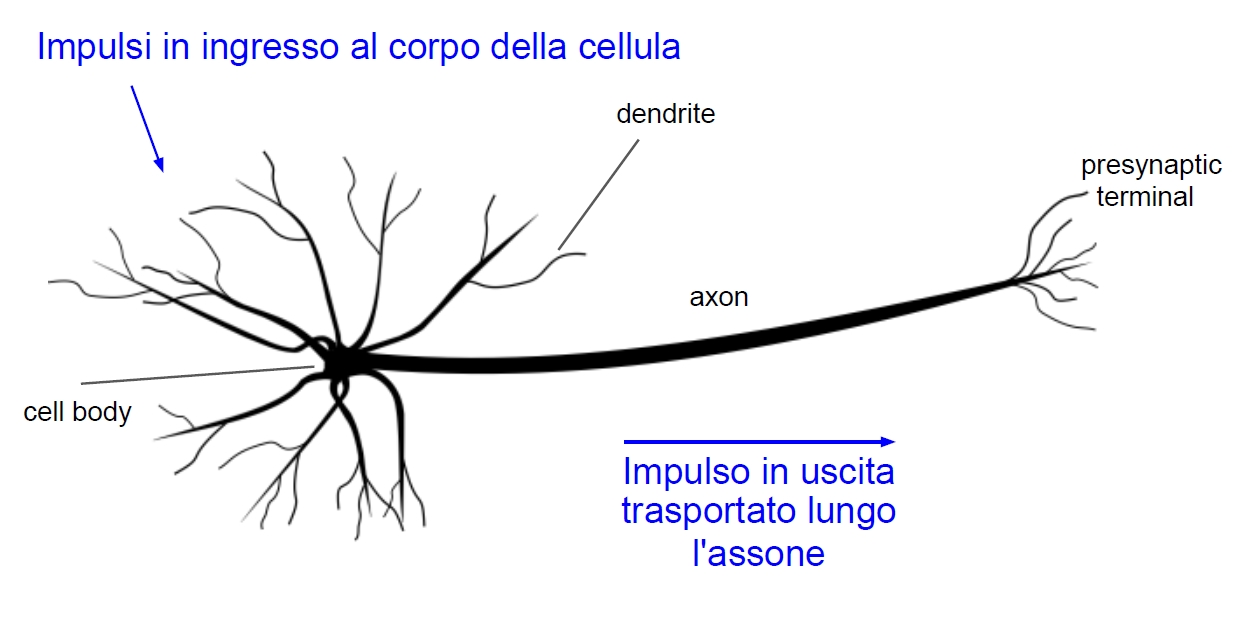
\includegraphics[width=\textwidth]{neuroneBiologico}
\caption{Disegno di un neurone biologico}
\label{fig:neuroneBiologico}
\end{subfigure}
\rulesep
\begin{subfigure}[b]{0.48\textwidth}
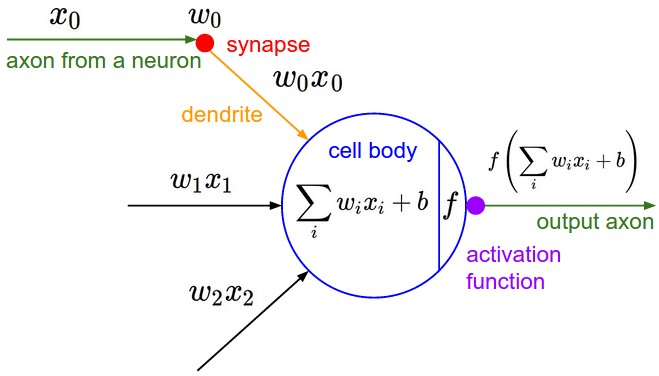
\includegraphics[width=\textwidth]{neuroneComputazionale}
\caption{Modello computazionale di un neurone}
\label{fig:neuroneComputazionale}
\end{subfigure}
\caption{Neuroni. Immagini tratte da: (a) \protect\url{https://thenounproject.com/term/neuron/214105/}, (b) \cite{cs231n}}
\label{fig:neurone}
\end{figure}

Ogni neurone si comporta quindi come la composizione di una funzione di attivazione $g$ con una funzione lineare (affine) $f(\mathbf{x}; \mathbf{w}, b)=\mathbf{w}^\top\mathbf{x}+b$; evidentemente, uno strato composto da neuroni si comporta come un classificatore lineare (par. \ref{classificatoreLineare}): ogni neurone di un certo strato $i$ aggiunge una riga alla matrice $\mathbf{W}^{(i)}$ dei pesi ed una al vettore $\mathbf{b}^{(i)}$ dei bias, associati a quello strato.\\

\subsection{Architettura delle reti neurali artificiali}
\label{architetturaANN}
Le reti neurali sono modellate come collezioni di neuroni connessi in un grafo aciclico diretto\footnote{in inglese \textit{direct acyclic graph} (DAG); particolare grafo orientato che non ha cicli diretti, ovvero comunque scegliamo un vertice del grafo non possiamo tornare ad esso percorrendo gli archi del grafo.}, organizzati in strati distinti.

Le architetture più "standard" delle reti neurali sono costituite da uno strato di input, uno o più \textbf{strati completamente connessi} (\textit{fully connected (FC) layer}) nei quali ciascun neurone è connesso a tutti i neuroni dello strato precedente e non esistono connessioni tra i neuroni dello stesso strato, ed infine uno strato di output. La fig. \ref{fig:esempioANN} mostra un esempio di rete neurale con soli layer FC.

\begin{figure}[h]
\centering
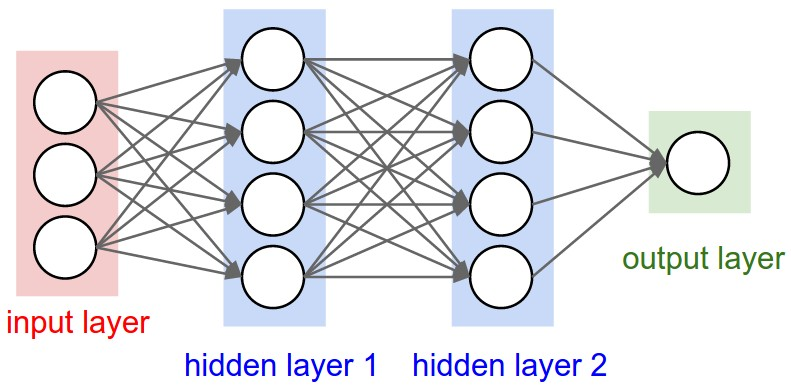
\includegraphics[width=0.7\textwidth]{esempioANN}
\caption{Una rete neurale con 3 strati (convenzionalmente non si conta quello di input) di cui due nascosti (\textit{hidden layers}) con 4 neuroni ciascuno e uno di output con un solo neurone.}
\label{fig:esempioANN}
\end{figure}

I valori reali assunti dai neuroni sono chiamati \textbf{attivazioni} dei neuroni.
Nei problemi di classificazione delle immagini (par. \ref{objectRecognition}), lo strato di input contiene neuroni in numero esattamente uguale a $hwc$, essendo le immagini accettate in input dalla rete di risoluzione $w\times h$ e con $c$ canali di colore. Ogni neurone contiene uno dei tre valori scalari che compongono un pixel. I neuroni dello strato di output sono in numero uguale a $|Y|$, il numero di categorie di oggetti che si possono classificare.

Spesso i neuroni dell'output layer non adoperano una funzione di attivazione (possiamo immaginare che usino la funzione identità). Nel caso di reti che svolgono un task di classificazione di immagini, come nel nostro caso, i valori delle attivazioni dei neuroni di output sono immessi nella funzione softmax per calcolare la distribuzione di probabilità da attribuire ad ogni classe di oggetti.

Le dimensioni di una rete neurale possono essere misurate con diverse metriche, tra cui il numero di neuroni o, più comunemente, il numero di parametri addestrabili. Ad esempio, la rete rappresentata in fig. \ref{fig:esempioANN} ha $4+4+1=9$ neuroni e quindi $3\times 4 + 4\times 4 + 4\times 1 = 32$ pesi e $4+4+1$ bias, per un totale di 41 parametri addestrabili.

Una rete neurale con strati completamente connessi può rappresentare una famiglia di funzioni (vettoriali di variabile vettoriale) parametrizzati dai pesi della rete.
È stato dimostrato \cite{approximation} che una rete neurale feedforward con un layer di output lineare e
almeno un hidden layer che abbia una funzione di attivazione tra quelle elencate in
precedenza può approssimare una qualsiasi funzione continua su un insieme chiuso e limitato di
$\R^{n}$ con un errore arbitrario.
Questo teorema fornisce una giustificazione teorica molto generica del funzionamento
delle reti neurali, ma non specifica nessun dettaglio riguardante l’architettura da utilizzare (es. numero di layer FC e numero di neuroni in ciascuno di essi)
per poter ottenere un errore di approssimazione desiderato. Le scelte riguardanti il
numero di layer, il numero di pesi per ciascun layer, il tipo di connettività tra i neuroni,
le funzioni di attivazione, il layer di output, ecc. derivano quasi sempre da risultati
sperimentali piuttosto che teorici.

Tutti i parametri della rete che non sono addestrabili ma che sono invece scelti arbitrariamente dal progettista (es. numero di layer della rete, input size, numero di neuroni in ogni layer, ecc.) si chiamano \textbf{iperparametri} della rete (\textit{hyperparameters}). Il loro valore ottimale non può essere trovato matematicamente (o meglio, spesso risulterebbe computazionalmente difficile farlo) ma possono essere scelti con un processo \textit{trial and error}.

\section{Reti neurali convoluzionali}
\label{CNN}
Una rete neurale si dice \textbf{convoluzionale} (\textit{convolutional}) se, in almeno uno dei layers, è utilizzata un'operazione di convoluzione al posto della consueta moltiplicazione tra matrici.

Grazie alla natura dell'operazione di convoluzione (par. \ref{convoluzione}), le reti neurali convoluzionali si sono rivelate particolarmente adatte al riconoscimento di pattern sia all'interno di segnali monodimensionali come audio o testo sia all'interno di segnali bidimensionali come le immagini. Questo è il motivo principale per cui sono state adoperate nell'ambito del task di classificazione binaria di immagini oggetto del presente lavoro (par. \ref{esperimentoTL}).
Per il resto del presente lavoro, ci riferiremo a CNN che lavorano esclusivamente su immagini e che nel suo strato finale utilizza la funzione softmax per calcolare la distribuzione di probabilità associata ad ogni classe dello spazio delle classi.

Una rete neurale convoluzionale è costituita da uno stack di layers, mostrato in fig. \ref{fig:convnet}: in input c'è un'immagine e in output c'è un vettore contenente la distribuzione di probabilità relativa alle categorie di oggetti classificabili.\\

L'architettura di una CNN può comporsi di strati di tipologie diverse\footnote{Va comunque notato che esistono numerosi altri strati che non sono presentati in questa sede. Alcuni di questi sono descritti nei paragrafi sulle tre CNN usate negli esperimenti, a cui pertanto si rimanda. Per una descrizione accurata di molti altri tipi di layer si rimanda a \url{https://code.google.com/archive/p/cuda-convnet/wikis/LayerParams.wiki}}

\begin{itemize}
	\item Input: generalmente un'immagine di dimensioni contenute (es. $224\times 224$). (par. \ref{INPUT})
	\item \textit{Convolutional layer} (CONV): vengono eseguiti diversi filtraggi sull'input, in maniera indipendente l'uno dall'altro, cioè un certo numero di convoluzioni con lo stesso dato in input ma con diversi kernel. (par. \ref{CONV}). Viene prodotto un set di \textit{feature map}.
	\item \textit{Activation layer} (detto anche \textit{ detector stage}): ciascun neurone dello strato precedente è passato ad una funzione di attivazione, tipicamente la ReLU. (par. \ref{RELU})
	\item \textit{Pooling layer} (POOL): viene eseguito un sottocampionamento dell'immagine attraverso una statistica riassuntiva delle regioni. (par. \ref{POOL})
	\item \textit{Fully-Connected layer} (FC): già descritti nella trattazione sulle reti neurali classiche; nell'ambito delle CNN sono finalizzati ad effettuare la classificazione vera e propria a partire dalle \textit{feature} estratte dai livelli convoluzionali precedenti. (par. \ref{FC})
	\item \textit{Softmax layer}: applica la funzione di attivazione softmax alla fine della rete, per calcolare la distribuzione di probabilità delle classi da predire. (par. \ref{SOFTMAX}
\end{itemize}

L'architettura di una CNN può prevedere una concatenazione di layer in serie (si parla in quest caso di \textit{series networks}, es. AlexNet par. \ref{alexnet}) ma anche una serie di modifiche che portano certi layer a funzionare in parallelo tra loro (ad es. il modulo \textit{inception} di GoogLeNet, par. \ref{inception}) o che comunque alterano il flusso lineare dell'informazione attraverso la rete mediante diramazioni (ad es. le \textit{skip connections} in ResNet, par. \ref{residualBlock}).

In questo modo, una rete CNN associa l'immagine in ingresso alla distribuzione di probabilità associata alle categorie classificabili.

Si noti che alcuni livelli contengono parametri e altri no. In particolare, i livelli Convolutional e Fully-Connected eseguono trasformazioni che sono funzione non solo delle attivazioni nel volume di input, ma anche dei parametri (i pesi e i bias dei neuroni). Invece, gli strati di attivazione e pooling implementeranno una funzione fissa, senza parametri addestrabili. I parametri degli strati CONV e FC vengono appresi in fase di addestramento attraverso l'applicazione dell'algoritmo di ottimizzazione \textit{stochastic gradient descent}, in modo che la distribuzione calcolati all'ultimo livello siano coerenti con le etichette del \textit{training set} per ogni immagine.

\begin{figure}[h]
	\centering
	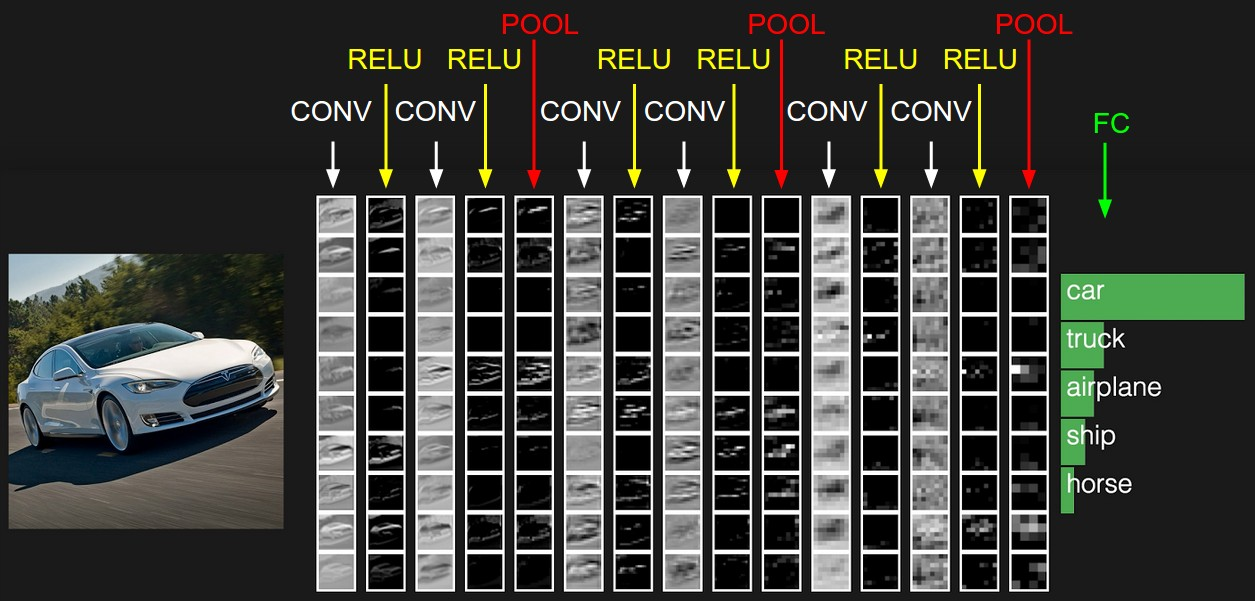
\includegraphics[width=0.7\linewidth]{convnet}
	\caption[Esempio di rete CNN]{Le attivazioni di un esempio di architettura ConvNet. Il volume iniziale memorizza i pixel dell'immagine in input (a sinistra) e l'ultimo volume memorizza la probabilità per ogni classe (a destra). Ogni volume di attivazioni lungo il percorso di elaborazione è mostrato come una colonna, in cui ogni immagine è una mappa bidimensionale di attivazione (vd. par. \ref{CONV}).}
	\label{fig:convnet}
\end{figure}

\subsection*{Volumi di attivazioni}
Come detto, le reti neurali convoluzionali ricevono in input delle immagini. Questo rende possibile un più "sensato" ed intuitivo arrangiamento dei neuroni nei vari layer. I neuroni sono infatti arrangiati in \textbf{volumi tridimensionali di attivazioni}. Così come le immagini hanno pixel arrangiati lungo la lunghezza, l'altezza e i canali di colore (profondità) dell'immagine, i neuroni di un certo strato possono essere arrangiati spazialmente lungo le stesse tre dimensioni. Allora si può dire che la rete opera una serie di trasformazioni che portano da un volume di attivazioni iniziale (quello determinato dall'immagine $w\times h\times 3$) ad uno finale: lo strato $i$-esimo trasforma il volume di attivazioni $i-1$-esimo nel volume $i$-esimo per mezzo di una funzione differenziabile.

Si veda la fig. \ref{fig:volume}. Al variare dell'indice $d$ del volume, che indica la terza dimensione del volume (la profondità, o \textit{volume depth}), si può univocamente identificare una sezione bidimensionale del volume, che chiameremo \textbf{mappa di attivazioni} (\textit{activation map}, anche detta \textit{depth slice}). In figura, ogni mappa di attivazioni è una griglia che contiene $a\times b$ neuroni.

\begin{figure}[h!]
\centering
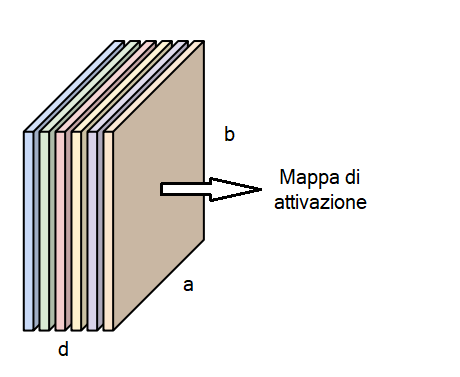
\includegraphics[width=0.4\textwidth]{volume}
\caption{Volume di attivazioni $a\times b\times d$}
\label{fig:volume}
\end{figure}


Si descrivono nel seguito con maggiore dettaglio i singoli layer, con le relative tecniche di implementazione in Matlab, utilizzate nel presente lavoro (par. \ref{esperimentoTL}).
Ogni tipo di layer esiste in Matlab come un tipo di dato complesso a se stante, ciascuno con la propria funzionalità.

In Matlab è possibile definire l'architettura di una CNN in due modi diversi:
\begin{enumerate}
\item Le reti i cui layer sono tutti "in serie" tra loros (es. AlexNet, par. \ref{alexnet}) sono rappresentate da un oggetto di tipo \verb|SeriesNetwork|, il quale contiene come campo un array di tipo \verb|Layer| che contiene (in ordine) gli strati della rete.
\item Le reti che hanno in generale un grafo aciclico diretto ma non in serie (es. GoogLeNet, par. \ref{googlenet}, ResNet-18 e 50, par. \ref{resnet}) sono rappresentate da un oggetto di tipo \verb|DAGNetwork|, il quale oltre al campo di tipo \verb|Layer| sopra citato contiene anche un altro campo di tipo \verb|table| di dimensioni $p\times 2$, dove $p$ è il numero di connessioni da stabilire tra i layer e le due colonne specificano rispettivamente il layer di partenza e quello di arrivo di ciascuna connessione.
\end{enumerate}

Entrambi questi oggetti possono essere passati come argomento della funzione \verb|trainNetwork| al fine di addestrare la rete.

\subsection{Input Layer}
\label{INPUT}
Rappresenta il layer di input alla rete per immagini 2D.
\begin{verbatim}
layer = imageInputLayer(inputSize,'Property',Value)
\end{verbatim}
\begin{itemize}
	\item \verb|inputSize| 
	
	Dimensione delle immagini in input, specificata come un vettore riga di 3 interi \verb|[h w c]|, con \verb|hxw| dimensione dell'immagine e \verb|c| numero di canali. Nel caso di immagini RGB, \verb|c| deve essere pari a 3.
	
	\item \verb|'Normalization', 'zero-centered'| oppure \verb|'none'|
	
	Specifica la trasformazione dei dati applicata in questo layer. Di default, viene applicata una centratura dei dati intorno allo zero, sottraendo l'immagine media del training set da ogni immagine di input. L'immagine media viene calcolata automaticamente a tempo di training dalla funzione \verb|trainNetwork|. In alternativa è possibile specificare esplicitamente l'immagine media da usare come parametro \verb|'AverageImage'| 
\end{itemize}

\subsection{Convolution Layer}
\label{CONV}
Il layer di convoluzione è il "cuore" delle reti neurali convoluzionali, in cui vengono effettuate importanti operazioni di filtraggio. Per ogni finestra dell'input, viene eseguita un'operazione di convoluzione (tridimensionale) tra il volume di attivazione $a\times b\times c$ e un kernel $h\times k\times c$, e per ogni mappa di attivazione ottenuta si aggiunge ai neuroni di quella mappa un termine di bias (vettore di bias $1\times 1\times c$) (fig. \ref{fig:cr}).

\begin{figure}[h]
	\centering
	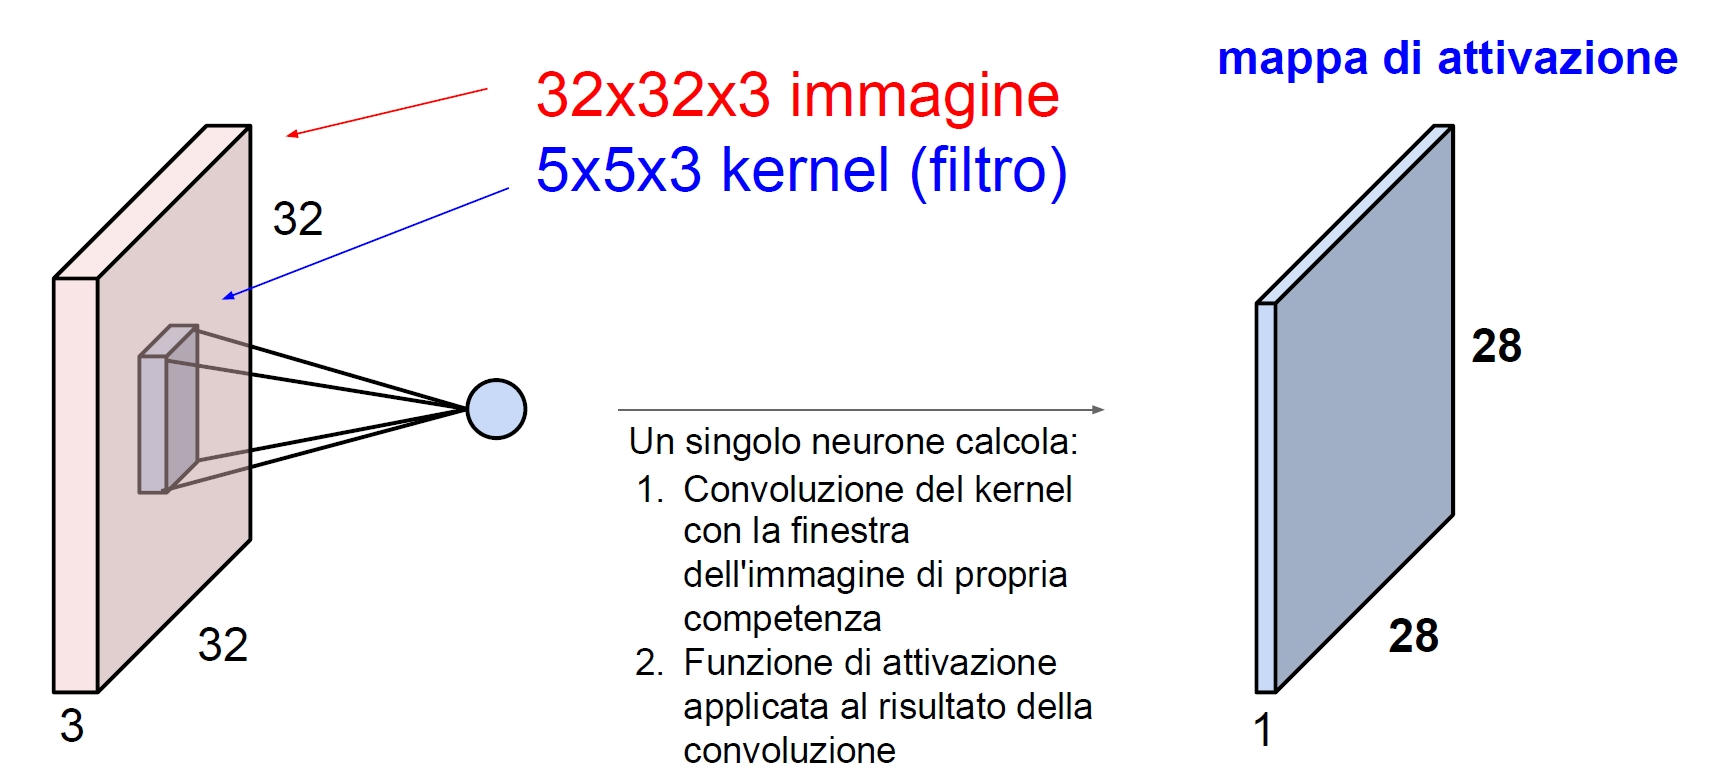
\includegraphics[width=0.7\linewidth]{CR}
	\caption[Convolution layer in una rete neurale convoluzionale]{Esempio di computazione di un neurone attraverso un layer di convoluzione e di attivazione. Utilizzando una convoluzione valida con stride pari a 1 e senza input padding, la convoluzione di un'immagine $32\times32\times3$ con un filtro $5\times5\times3$ produce una matrice $28\times28\times1$, cui viene applicata la funzione d'attivazione scelta per ottenere una activation map. Tutti i $28\times28$ neuroni impiegati per il calcolo di ogni singolo elemento che compone la mappa di attivazione utilizzano lo stesso filtro, cioè un kernel con gli stessi parametri (\textbf{parameter sharing})}
	\label{fig:cr}
\end{figure}

In Matlab, la creazione del layer avviene attraverso la funzione \texttt{\justify{convolution2dLayer}}:

\begin{verbatim}
layer = convolution2dLayer(filterSize,numFilters,'Property',Value)
\end{verbatim}

Gli argomenti sono:

\begin{itemize}
	\item \verb|filterSize|
	
	Dimensione del kernel, specificato come un intero \verb|F| per ottenere un filtro quadrato \verb|F x F|. Se si vogliono utilizzare dimensioni differenti (filtro in generale rettangolare) è possibile specificare un vettore \verb|[h w]|.
	
	\item \verb|numFilters|
	
	Numero dei filtri, specificato come un intero positivo \verb|K|. Questo parametro corrisponde al numero di neuroni nel layer di convoluzione che sono connessi alla stessa regione dell'input. Il volume di output avrà esattamente \verb|K| livelli di profondità (cioè \verb|K| mappe di attivazioni). (fig. \ref{fig:ca})
\end{itemize}

\begin{figure}[h]
	\centering
	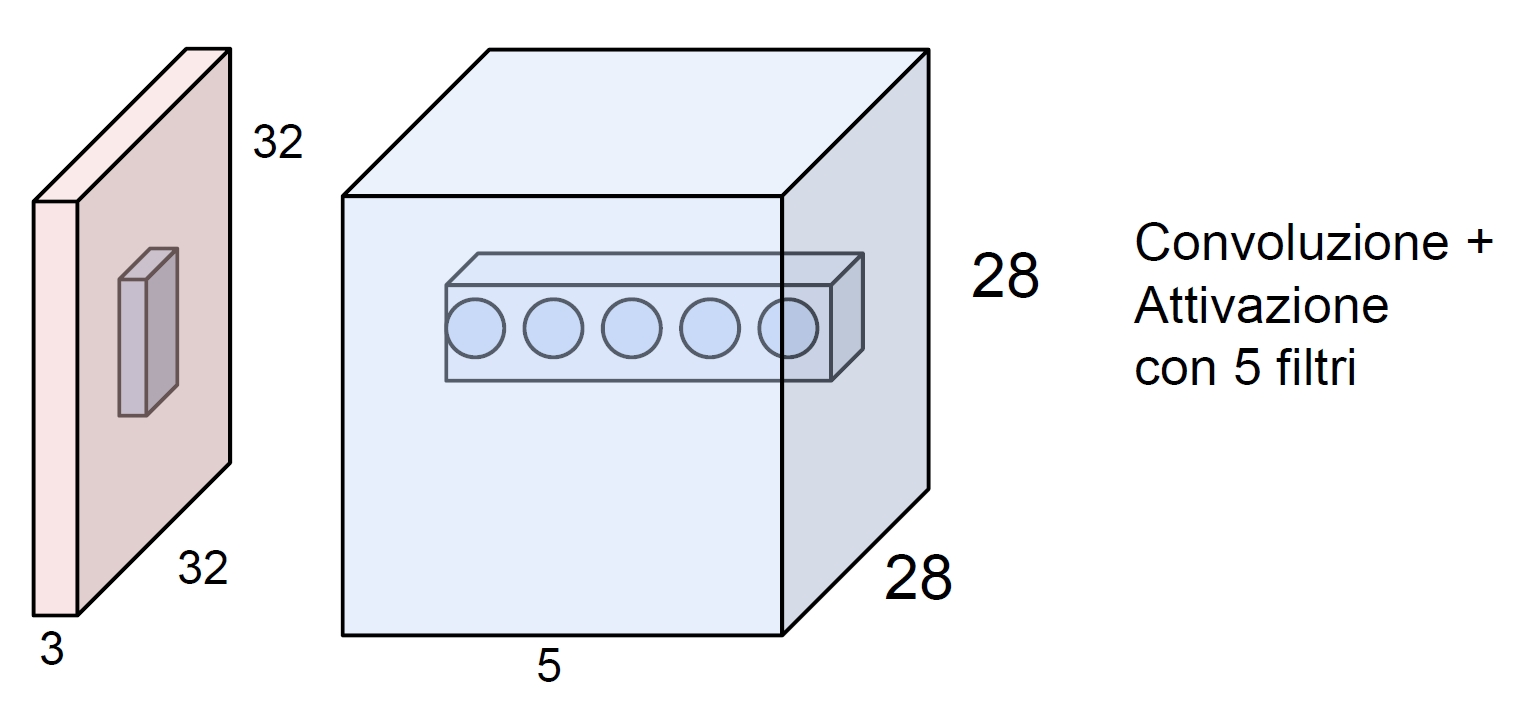
\includegraphics[width=0.7\linewidth]{CA}
	\caption[Output di un Convolution Layer]{I 5 neuroni mostrati applicano un diverso filtro (un kernel con diversi parametri) alla stessa regione spaziale dell'immagine in input, in maniera indipendente l'uno dall'altro.}
	\label{fig:ca}
\end{figure}

Gli eventuali parametri che possono essere specificati sono:

\begin{itemize}
	\item \verb|'Stride', S|
	
	Parametro che regola lo scorrimento della finestra del filtro sull'input. Se si specifica un intero positivo \verb|S|, gli scorrimenti della finestra sono caratterizzati da una traslazione di \verb|S| pixel in orizzontale e di \verb|S| pixel in verticale. Se si vogliono utilizzare traslazioni differenti rispetto alle due dimensioni è possibile specificare un vettore \verb|[h w]|.
	
	\item \verb|'DilationFactor', L|
	
	Fattore che specifica una convoluzione "dilatata". Se si specifica un intero positivo \verb|L| maggiore di 1, è come se il filtro venisse ampliato inserendo \verb|L-1| zeri tra ogni elemento. Il risultato è quello di ampliare la dimensione del campo ricettivo (\textit{receptive field}) rispetto all'input. Se si vuole utilizzare una dilatazione differente rispetto alle due dimensioni è possibile specificare un vettore \verb|[h w]|. (fig. \ref{fig:dilation})
	
\begin{figure}[h]
	\centering
	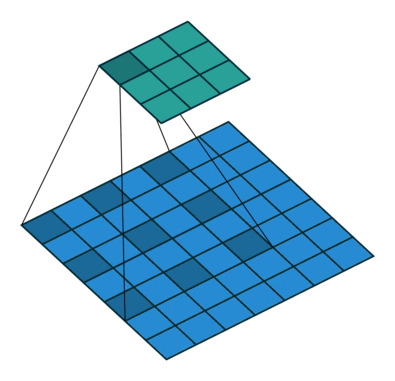
\includegraphics[width=0.3\linewidth]{dilation}
	\caption{Dilation di fattore L=2}
	\label{fig:dilation}
\end{figure}
	
	\item \verb|'PaddingSize', [t b l r]|
	
	Dimensione del padding da applicare all'input, specificata come un vettore di quattro interi positivi. Indicano rispettivamente il numero di righe nulle da aggiungere in alto (top) e in basso (bottom) e il numero di colonne nulle da aggiungere a sinistra (left) e a destra (right). Di default, il padding è nullo.
	
	\begin{figure}[h]
	\centering
	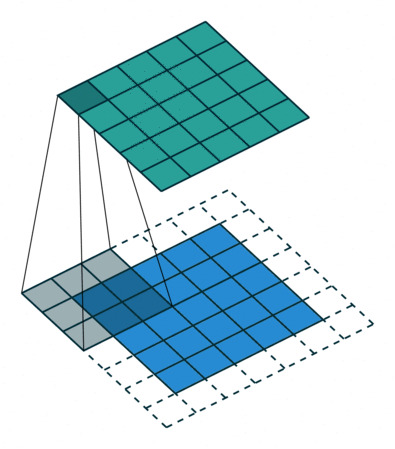
\includegraphics[width=0.3\linewidth]{padding}
	\caption{Padding con t=b=l=r=1}
	\label{fig:padding}
\end{figure}
	
	\item \verb|'PaddingMode', 'manual'| oppure \verb|'same'|
	
	Questa proprietà è utile se si vuole preservare la dimensione dell'input attraverso un layer di convoluzione. Specificando il valore \verb|'same'|, infatti, viene calcolato automaticamente il valore della dimensione del padding adatto a perseguire tale scopo. Per un filtro quadrato di dimensione \verb|F|, ad esempio, è necessario applicare un padding uniforme \verb|[P P P P]| con \verb|P = (F-1)/2|.
	
	\item \verb|'NumChannels','auto'| oppure \verb|n|
	
	Numero di canali (livelli di profondità) per ciascun filtro. Di default, questo parametro è sempre uguale alla profondità del tensore di input al livello di convoluzione
	
	\begin{figure}[h]
		\centering
		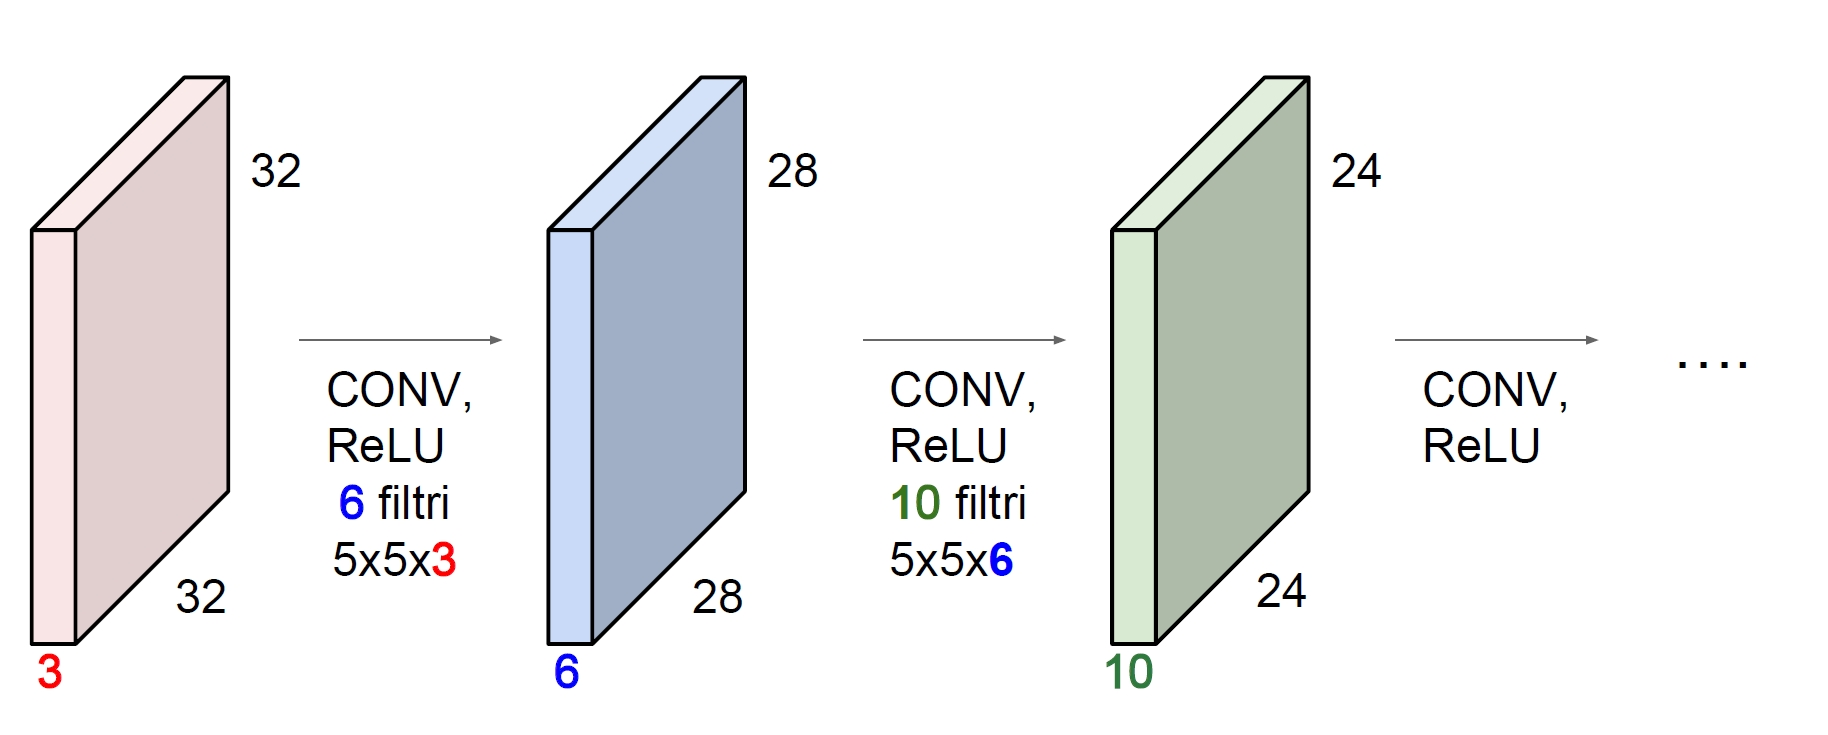
\includegraphics[width=0.7\linewidth]{channels}
		\caption[Profondità dei filtri attraverso una CNN]{La figura mostra come la profondità dei filtri di ogni livello di convoluzione debba essere equivalente alla profondità dell'input del rispettivo livello}
		\label{fig:channels}
	\end{figure}

	\item \verb|'Weights', W|
	
	\verb|Weights| è l'array contenente i pesi del layer, ovvero i parametri che definiscono le convoluzioni e che vengono appresi dalla rete durante la fase di addestramento. Se l'input al layer è di profondità \verb|D_i|, il kernel è di dimensione \verb|F| e il numero di filtri è pari a \verb|K|, allora \verb|Weights| sarà un array \verb|4-D single| di dimensione \verb|F|$ \times $\verb|F|$ \times $\verb|D_i|$ \times $\verb|K|, in cui la quarta dimensione indicizza ogni filtro. Specificando questa proprietà, è possibile inizializzare i pesi con un vettore a propria scelta \verb|W|.
	
	\item \verb|'Bias', B|
	
	\verb|Bias| è l'array contenente i parametri di bias, ovvero i parametri che vengono sommati al risultato delle convoluzioni, anch'essi appresi dalla rete durante la fase di addestramento. Se \verb|K| è il numero di filtri applicato nel layer, allora \verb|Bias| sarà un array \verb|3-D single| di dimensioni \verb|1|$\times$\verb|1|$\times$\verb|K|
	
	\item \verb+'WeightsInitializer','glorot'|'he'| 'narrow-normal'|'zeros'|'ones'+
	
	Funzione utilizzata per l'inizializzazione dei pesi in \verb|Weights|. Le alternative sono:
	
	\begin{itemize}
		\item \verb|'glorot'|: generatore pseudocasuale utilizzato di default, con una distribuzione uniforme a media nulla e varianza \verb|2/(numIn+numOut)|, con \verb|numIn=F|$\times$\verb|F|$\times$\verb|D_i| e \verb|numOut=F|$\times$\verb|F|$\times$\verb|K|
		
		\item \verb|'he'|: generatore pseudocasuale di una distribuzione uniforme a media nulla e varianza \verb|2/numIn|, con \verb|numIn=F|$\times$\verb|F|$\times$\verb|D_i|
		
		\item \verb|'narrow-normal'|: generatore pseudocasuale di una distribuzione uniforme a media nulla e varianza 0.01
		
		\item \verb|'zeros'|: inizializza con tutti zeri
		
		\item \verb|'ones'|: inizializza con tutti 1
		
		\item \verb|function handle|: utilizza una funzione \textit{custom}
		
	\end{itemize}
	
	\item \verb+'BiasInitializer','zeros'|'narrow-normal'|'ones'|function handle+
	
\end{itemize}

Learning rate (locale) e regolarizzazione:

\begin{itemize}
	\item \verb|'WeightLearnRateFactor',alfa|
	
	Fattore da moltiplicare per il parametro learning rate globale relativo all'apprendimento dei pesi, di default pari a 1
	
	\item \verb|'BiasLearnRateFactor',beta|
	
	Fattore da moltiplicare per il parametro learning rate globale relativo all'apprendimento dei bias, di default pari a 1
	
	\item \verb|'WeightL2Factor',lambda1|
	
	Fattore da moltiplicare per il parametro globale di regolarizzazione L2 relativo all'apprendimento dei pesi, di default pari a 1
	
	\item \verb|'BiasL2Factor',lambda2|
	
	Fattore da moltiplicare per il parametro globale di regolarizzazione L2 relativo all'apprendimento dei bias, di default pari a 1
	
\end{itemize}

\subsection{Activation layer}
\label{RELU}
Il layer di attivazione è implementato, nel caso di funzione ReLU (l'unica che utilizzeremo in questo lavoro di tesi), mediante \verb|relulayer|.

\subsection{Pooling layer}
\label{POOL}
Una funzione di pooling opera un sottocampionamento sull'immagine, come mostrato in figura \ref{fig:pooling}.  Ogni regione di una certa dimensione dell'immagine in input (es. $4\times4$) viene ridotta ad un unico pixel, il cui valore è calcolato tramite una statistica riassuntiva della regione di partenza (es. max, media, norma L2).
\begin{figure}[h!]
\centering
\begin{subfigure}[b]{0.48\textwidth}
\centering
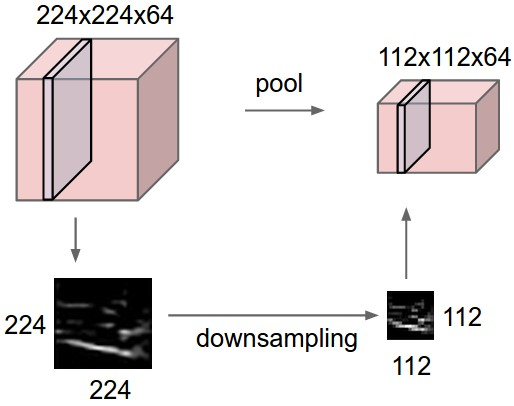
\includegraphics[width=\textwidth]{pool}
\caption{}
\end{subfigure}

\begin{subfigure}[b]{0.48\textwidth}
\centering
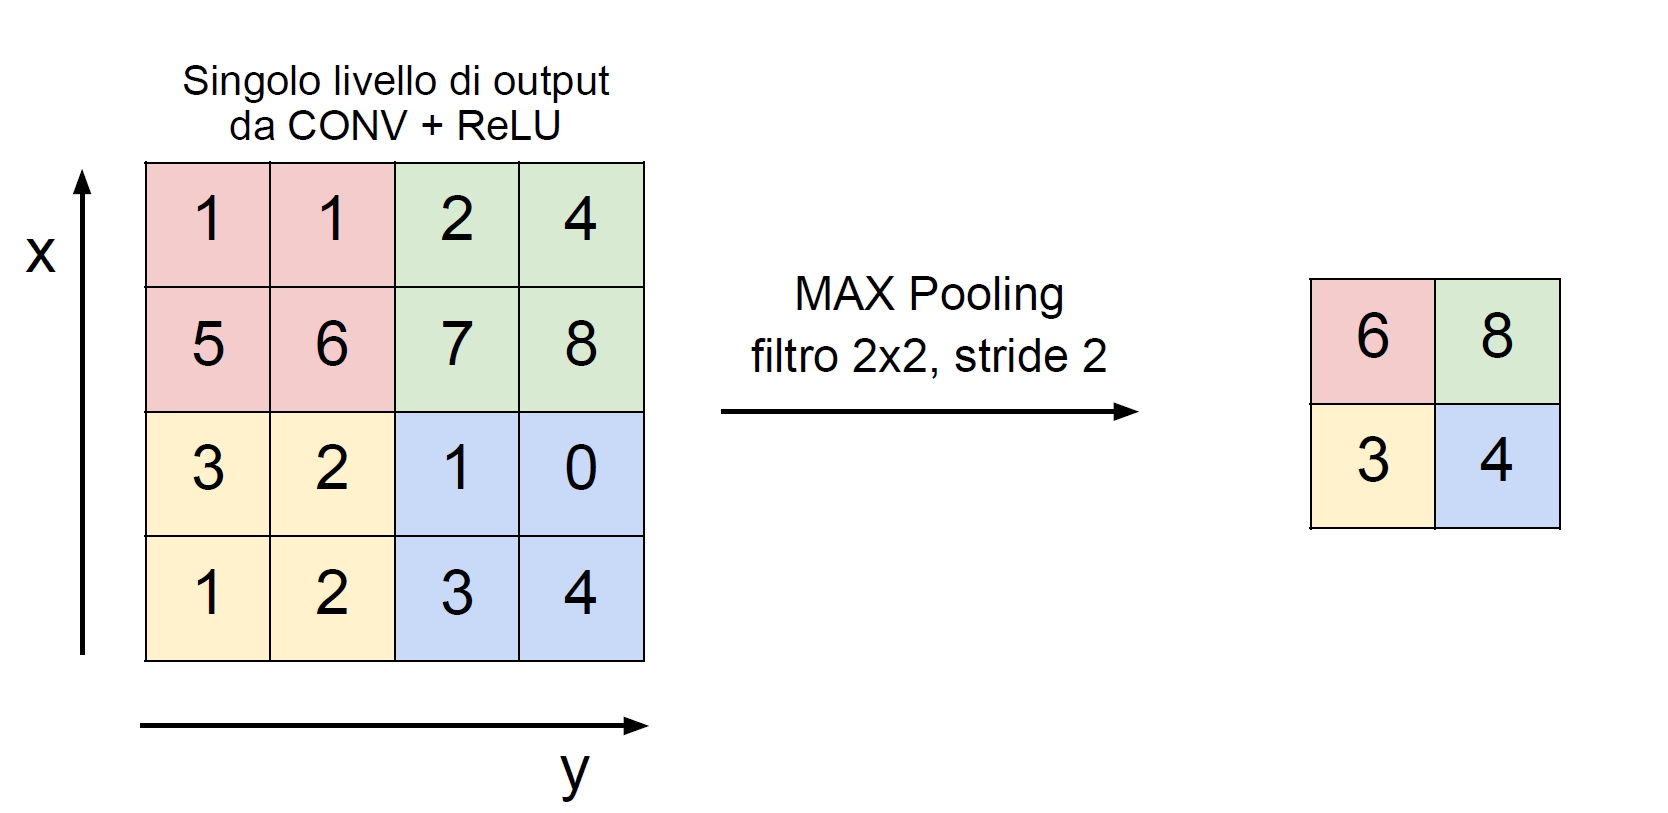
\includegraphics[width=\linewidth]{pooling}
\caption{}
\end{subfigure}
\caption{Operazione di pooling: (a) effetto di downsampling; (b) calcolo del max pooling}
\label{fig:pooling}
\end{figure}

L'utilità del pooling è quella di ridurre progressivamente la dimensione spaziale dei volumi che "scorrono" nell'architettura, per ridurre la quantità di parametri e di calcolo nella rete. Tipicamente, l'operazione è eseguita mediante un filtro di dimensioni $2\times 2$ (o anche $3\times 3$) applicato con uno stride di 2. Il risultato è quello di ridurre del 75\% il numero delle attivazioni propagate. Ogni operazione di max pooling richiederebbe in questo caso un massimo di 4 numeri (regione $2\times 2$). La dimensione della profondità del tensore di attivazione rimane invariata.\\

La funzione utilizzata per la sua creazione è \verb|maxPooling2dLayer|

\begin{verbatim}
layer = maxPooling2dLayer(poolSize,'Property',Value)
\end{verbatim}
\begin{itemize}
	\item \verb|PoolSize|
	
	Dimensione delle regioni di pooling, specificata come un intero positivo \verb|F|, in caso di finestra quadrata oppure un vettore di due interi positivi \verb|[h w]|, con \verb|h| altezza e \verb|w| larghezza della finestra
\end{itemize}
Le proprietà di questo layer sono del tutto analoghe a quelle del  \verb|convolution2dLayer| per ciò che riguarda il comportamento ai bordi e le modalità di traslazione della finestra. Si possono perciò parimenti specificare le proprietà \verb|'Stride'|, \verb|'PaddingSize'| e \verb|'PaddingMode'|.

\subsection{Fully Connected Layer}
\label{FC}
Moltiplica l'input per un tensore di pesi (di dimensioni pari a quelle del volume in input al layer) e aggiunge un vettore bias (di dimensione pari al numero di neuroni del layer FC). Ciascun neurone è connesso con tutti i neuroni del layer precedente. Un esempio numerico è mostrato in fig. \ref{fig:fc}.\\

I layer fully connected si implementano in Matlab con:
\begin{verbatim}
layer = fullyConnectedLayer(outputSize,'Property',Value)
\end{verbatim}

dove:

\begin{itemize}
	\item \verb|outputSize|
	
	Dimensione di uscita del fully connected layer, specificato come un numero intero positivo \verb|C|. Nel caso in cui il layer sia posto alla fine della rete (layer FC di classificazione, che fornisce valori alla funzione softmax finale), \verb|C| deve essere uguale al numero delle classi $|Y|$ da individuare all'interno del dataset.
\end{itemize}

\begin{figure}[h]
	\centering
	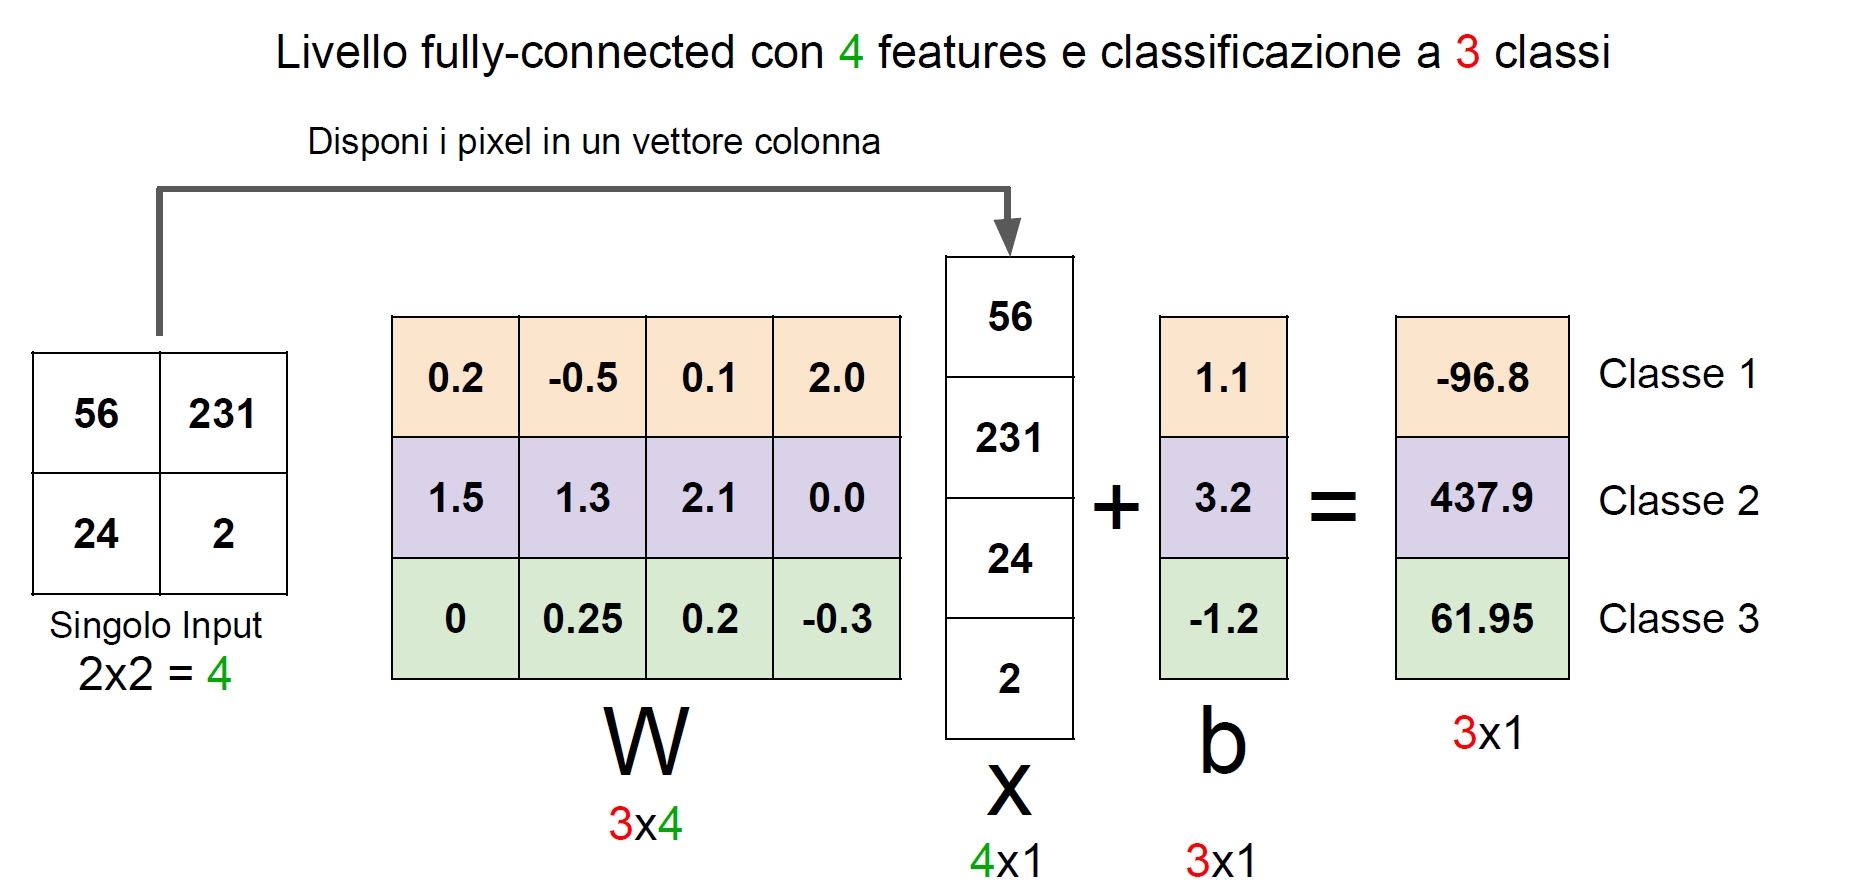
\includegraphics[width=0.7\textwidth]{fc}
	\caption{Esempio numerico di livello fully connected con un singolo input}
	\label{fig:fc}
\end{figure}

\subsection{Softmax layer}
\label{SOFTMAX}
La funzione di attivazione finale softmax, inserita in coda all'ultimo fully connected layer, è implementata mediante \verb|softmaxLayer|.



\section{Image preprocessing e augmentation}
\label{augmentation}

La tecnica dell'\textbf{\textit{image preprocessing}} consiste in generale nel trasformare le immagini (esempi) di un dataset per mezzo di operazioni sulle sue feature. Tipicamente, queste operazioni sono applicate alle immagini di un training set prima che ci si serva di esso per addestrare un classificatore, ma possono essere applicate anche sui test set.
Le trasformazioni possono includere centraggio delle feature, normalizzazione, traslazioni, rotazioni, riflessioni, scalatura, e così via.

In generale, ci sono due motivi per cui si vuole effettuare il preprocessing di un training set:

\begin{itemize}
\item Rendere le immagini più semplici da elaborare da parte di una rete neurale. Ad esempio, il centraggio e la normalizzazione delle feature possono essere utili ad evitare eventuali problemi di overflow e stabilità numerica nelle operazioni eseguite dalla rete.

\item Migliorare la capacità di generalizzazione del modello. Nel caso dell'\textit{image classification}, le classi rispetto a cui il classificatore deve produrre un output sono infatti spesso invarianti rispetto ad un'ampia varietà di trasformazioni negli input, facilmente realizzabili. Operazioni geometriche come traslazioni, rotazioni, riflessioni, scalatura (già viste nel par. \ref{trasformazioni}) possono essere implementate come semplici operazioni sui pixel (trasformazioni affini) e si rivelano particolarmente utili (se eseguite in modo casuale ma accorto) per la riduzione dell'errore di generalizzazione della maggior parte di modelli di computer vision.
\end{itemize}

Tra le forme di preprocessing più comunemente utilizzate su un'immagine (esempio) $\mathbf{x}$ di un training set per assolvere al primo dei due obiettivi del preprocessamento delle immagini citiamo:

\begin{itemize}
\item \textbf{Sottrazione della media} (\textit{mean subtraction}), che consiste nel sottrarre ad ogni feature dell'esempio la media di tutte le feature. L'interpretazione geometrica di questa operazione è il centraggio delle feature attorno allo 0.

\item \textbf{Normalizzazione} dei pixel. Solitamente un'immagine a colori rappresentata come un tensore a 3 canali RGB ha ogni pixel rappresentato da un intero senza segno di 1 byte, quindi nel range $[0,255]$. Si può quindi fare in modo che tutti i pixel siano normalizzati in un range ragionevole, come $ [0,1] $ oppure $ [-1,1] $.
Un'ulteriore forma di normalizzazione è la divisione di ogni feature per la deviazione standard di tutte le feature (operazione che va applicata solo dopo il centraggio attorno allo 0 delle feature, con la sottrazione della media).
\end{itemize}

Il secondo obiettivo del preprocessamento è particolarmente critico nel caso in cui il training set a nostra disposizione è relativamente piccolo e poco eterogeneo (cioè con poca variabilità nelle immagini di una stessa classe). Spesso training set piccoli non sono sufficienti per addestrare la rete in maniera soddisfacente, rendendo il rischio di overfitting particolarmente concreto.

Al fine di aggirare questo problema si mette in campo una strategia di \textbf{\textit{image augmentation}}, una particolare forma di \textit{image preprocessing} che ha come scopo quello di ingrandire (\textit{augment}) il training set con nuovi esempi, generati in vario modo a partire da quelli del training set originale.

Le trasformazioni di \textit{augmentation} sono in genere scelte in maniera casuale (con una certa probabilità per ciascuna) per ogni esempio da "aumentare", da un set di operazioni specificato a priori da chi addestra la rete.

Tra le operazioni di \textit{image augmentation} più comuni citiamo:

\begin{itemize}
\item Estrarre da ogni esempio dei ritagli rettangolari da posizioni differenti.
\item Applicare trasformazioni geometriche affini, quali quelle descritte nel par. \ref{trasformazioni}.
\item Applicare distorsioni fotometriche e cromatiche di vario tipo.
\end{itemize}

Bisogna comunque osservare che per dataset grandi ed eterogenei solitamente si fanno poche operazioni di augmentation di questo tipo, poichè si lascia imparare al modello a quale tipo di fattori di variazione esso deve essere invariante.\\

In Matlab è possibile ottenere la versione aumentata di un dataset con un oggetto di tipo \verb|augmentedImageDatastore|. Esso consente di trasformare un dataset, definito in un oggetto \verb|imageDatastore| (vd. par. \ref{datastore}) con eventuali operazioni di preprocessing e augmentation specificate in un oggetto di tipo \verb|imageDataAugmenter|.
Un oggetto \verb|augmentedImageDatastore| può essere passato semplicemente come argomento della funzione \verb|trainNetwork| (vd. par. \ref{addestramento}), per essere utilizzato come \textit{training set} di una rete neurale. In tal caso, per ogni \textit{epoch} (quindi a \textit{runtime}), i dati di training vengono casualmente perturbati e ridimensionati all'input size della rete\footnote{Il ridimensionamento è necessario affinché tutte le immagini rispettino la dimensione di input della rete neurale, che è fisso.}, in modo che ciascuna \textbf{\textit{epoch}} (epoca), cioè un ciclo di addestramento sull'intero training set, usi un training set leggermente diverso. Il numero effettivo di immagini usate per ciascuna \textit{epoch} non cambia. Le immagini trasformate non vengono memorizzate. L'\verb|imageInputLayer| di una CNN normalizza le immagini ad ogni \textit{epoch}, sottraendo un'intensità media costante calcolata un'unica volta, subito dopo la augmentation relativa alla prima \textit{epoch}. In fig. \ref{fig:augmentationTraining} viene mostrato il processo di addestramento di una rete neurale adoperando un augmentedImageDatastore.\\

\begin{figure}[h]
\centering
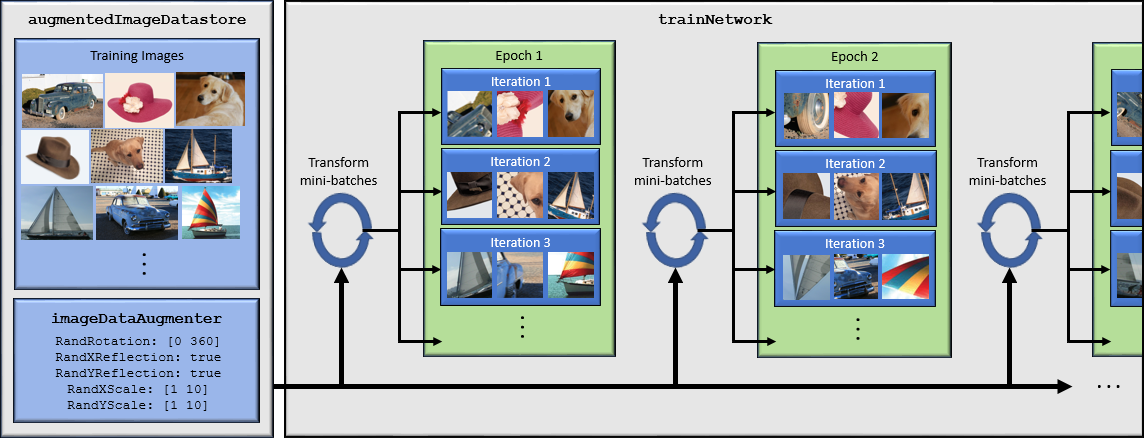
\includegraphics[width=0.9\textwidth]{augmentationTraining}
\caption{Processo di addestramento (mediante \textit{stochastic gradient descent} con dimensione del mini-batch = 3) in cui il training set è definito con un oggetto augmentedImageDatastore}
\label{fig:augmentationTraining}
\end{figure}

La creazione di un oggetto \verb|augmentedImageDatastore| avviene invocando la funzione

\begin{verbatim}
auimds = augmentedImageDatastore(outputSize,imds)
\end{verbatim}

Altri argomenti opzionali sono:

\begin{itemize}

	\item \verb|NumObservations|: numero totale di "osservazioni" nella collezione di immagini aumentate. Coincide con la lunghezza di ogni training \textit{epoch}, quindi coincide con l'omonima proprietà dell'oggetto \verb|trainingOptions| (vd. par. \ref{addestramento}) e può essere modificato solo di lì (proprietà READ-ONLY).
	
	\item \verb|Files|: oggetto \verb|cell array| contenente le directory delle immagini ereditate dall'oggetto \verb|imageDatastore| con cui è stato costruito)
	
	\item \verb|MiniBatchSize|: dimensione del mini-batch utilizzato durante l'addestramento dal metodo \textit{stochastic gradient descent} per il calcolo della funzione costo. Coincide con l'omonima proprietà dell'oggetto \verb|trainingOptions| e può essere modificato solo di lì (proprietà READ-ONLY).
	
	\item \verb|DataAugmentation|: oggetto di tipo \verb|imageDataAugmenter| che consente di definire trasformazioni di preprocessing da applicare alle immagini
	
	\item \verb|ColorPreprocessing|: eventuali conversioni \verb|'gray2rgb'| o \verb|'rgbtogray'| per fare in modo che tutte le immagini abbiano lo stesso numero di canali richieste dall'\verb|imageInputLayer| della rete neurale.
	
	\item \verb|OutputSize|: dimensione delle immagini di output, come vettore di due interi positivi. L'operazione di ridimensionamento è l'unica operazione di augmentation prevista di default, al fine di rendere le immagini compatibili con la dimensione di input specificata nell'\verb|imageInputLayer|
	
	\item \verb|OutputSizeMode|: metodo utilizzato per il ridimensionamento delle immagini
	
	\begin{itemize}
		\item \verb|'resize'|: le immagini vengono scalate utilizzando la interpolazione bilineare con antialiasing (operazione più veloce ma con risultati di qualità inferiore rispetto alla interpolazione bicubica utilizzata da \verb|imresize|. Evita distorsioni causate dalla interpolazione nearest-neighbor). Questa opzione è di default.
		\item \verb|'centercrop'|: viene effettuato un ritaglio al centro dell'immagine della dimensione specificata in \verb|OutputSize|
		\item \verb|'randcrop'|: viene effettuato un ritaglio in una posizione casuale dell'immagine della dimensione specificata in \verb|OutputSize|
	\end{itemize}
\end{itemize}

Se non è specificato come argomento un oggetto \verb|imageDataAugmenter|, l'unica operazione di preprocessing svolta è il ridimensionamento all'input size della rete.

La sintassi per creare un oggetto \verb|imageDataAugmenter| è:

\begin{verbatim}
aug = imageDataAugmenter('Property',Value,...)
\end{verbatim}

in cui è possibile definire le opzioni di \textit{image augmentation} esprimendo una o più coppie proprietà-valore. Tra le varie possibilità, citiamo solo quelle effettivamente utilizzate all'interno del presente lavoro:
\begin{itemize}
	\item \verb+'RandXReflection', true|false+ \newline\vspace{0.1mm}\verb+'RandYReflection', true|false+
	
	Ogni immagine subisce con una probabilità del 50\% una riflessione orizzontale (\verb|X|) oppure verticale (\verb|Y|)
	\item \verb|'RandRotation',[a b]|
	
	Applica una rotazione con un angolo, espresso in gradi, estratto da una distribuzione uniforme pseudocasuale nell'intervallo $[a,b]$
	\item \verb|'RandXTranslation',[a b]|\newline\vspace{0.1mm}\verb|'RandYTranslation',[a b]|
	
	Applica una traslazione orizzontale (\verb|X|) oppure verticale (\verb|Y|) all'immagine. L'entità della traslazione, misurata in pixel, è estratta da una distribuzione uniforme pseudocasuale nell'intervallo $[a,b]$
\end{itemize}

\section{Addestrare una rete neurale}
Per poter essere impiegata per risolvere un certo task, una rete neurale deve essere opportunamente addestrata. Addestrare una rete neurale significa individuare un set di valori per i parametri addestrabili della rete che le permettono di approssimare la funzione desiderata (cioè che le permettano di risolvere efficacemente il task).
Un addestramento efficace rende la rete capace di generalizzare in modo appropriato, cioè di dare risposte plausibili per input che non ha mai visto.\\

Riferendoci ad una rete che svolge un task di \textit{image classification} (ma si può facilmente estendere la spiegazione ad una ANN standard), l'addestramento della rete avviene in due diversi stadi: \textit{forward-pass} (propagazione in avanti) e \textit{backward-pass} (propagazione all'indietro).
\begin{itemize}
\item Nel \textit{forward-pass} a partire dalle immagini in input si calcolano di strato in strato tutti i volumi intermedi fino al volume finale, che permette la classificazione. Durante questa fase i valori dei parametri addestrabili sono tutti fissati.
\item Nel \textit{backward-pass} la risposta della rete (la distribuzione di probabilità della predizione) viene confrontata con l'uscita desiderata (la distribuzione di probabilità che assegna probabilità 1 alla effettiva classe di appartenenza dell'immagine e 0 alle rimanenti) ottenendo il segnale d'errore, calcolato per mezzo della funzione costo (par. \ref{loss}). L'errore calcolato è propagato nella direzione inversa rispetto a quella del \textit{forward-pass}. I parametri sono aggiornati ad ogni iterazione in modo da minimizzare la funzione costo, tramite un metodo di minimizzazione come la discesa stocastica del gradiente (par. \ref{SGD}), che calcola il gradiente della funzione costo rispetto ad ogni parametro con l'algoritmo di backpropagation (par. \ref{backpropagation}).
\end{itemize}

\subsection{Inizializzazione dei parametri}
\label{weights}
Prima di addestrare la rete, i parametri devono essere inizializzati con valori casuali, che saranno poi alterati durante il training.\\
Delle scelte comuni per i pesi sono:
\begin{itemize}
\item estrazione di un valore casuale della variabile aleatoria $\varepsilon \mathcal{X}$, dove $\varepsilon$ è piccolo (tipicamente 0.01) e $\mathcal{X}$ è la v.a. gaussiana standard (media nulla e varianza unitaria).
\item estrazione di un valore casuale della variabile aleatoria $\frac{\mathcal{X}}{\sqrt{n}}$, dove $\mathcal{X}$ è la v.a. gaussiana standard e $n$ è il numero di parametri associati al nodo a cui il parametro di cui si è estratta l'inizializzazione appartiene.
\item estrazione di un valore casuale della variabile aleatoria $\frac{\mathcal{X}}{\frac{2}{\sqrt{n}}}$, con le stesse variabili descritte al punto precedente
\end{itemize}

\subsection{Loss function}
\label{loss}
Abbiamo visto che una rete neurale per l'\textit{image classification} accetta in input un'immagine e restituisce un punteggio per ogni classe da predire, o equivalentemente una probabilità per ogni classe (calcolata dalla funzione di attivazione softmax). In fig. \ref{class_lin} si era visto che quel particolare classificatore lineare assegnava all'immagine di un gatto un punteggio molto alto alla classe 'cane' ed uno molto basso alla classe 'gatto', classificandola pertanto come 'cane'. Il set di parametri costituito da $\mathbf{W}$ e $\mathbf{b}$ non è molto buono. Per misurare l'entità dell'errore commesso dalla rete nella classificazione definiamo una \textbf{funzione costo} (\textbf{\textit{loss function}}) anche detta funzione obiettivo (\textit{objective}).

Tra le varie loss function che si possono adoperare, quella utilizzata nel presente lavoro è la \textbf{\textit{cross-entropy loss}}, che è quella tipica delle reti che sfruttano la funzione softmax per effettuare la predizione.
Dato un training set (eventualmente aumentato) $X$ contenente $|X|$ immagini $\mathbf{x}^{(i)}$ ($i=1,\dots,|X|$), ciascuna appartenente alla classe $i$-esima, uno spazio delle etichette $Y$ e una rete neurale che associa all'immagine $|Y|$ punteggi diversi $s_j$ per ciascuna classe $j$-esima ($j=1,\dots,|Y|$), si definisce cross-entropy loss relativa al training set $X$ la funzione
\[
L=\underbrace{\frac{1}{|X|}\sum_{i=1}^{|X|}L_i}_{\text{data loss}}+\underbrace{\lambda R(\mathcal{W})}_{\text{regularization loss}}
\]
dove
\begin{itemize}
\item \begin{align*}
L_i=-\log\left(\frac{e^{s_i}}{\sum\nolimits_{j}e^{s_j}}\right) & \text{ o equivalentemente} & L_i=-s_i+\log\left(\sum\nolimits_{j}e^{s_j}\right)
\end{align*}
è il contributo alla cross-entropy loss di un singolo esempio del dataset. Esso è tanto maggiore quanto più la rete si comporta "male" sull'esempio $\mathbf{x}^{(i)}$. Si noti che nella prima parentesi è utilizzata la funzione softmax($s_j$).

\item $\mathcal{W}$ è l'insieme di tutti i parametri addestrabili della rete.

\item $R(\mathcal{W})$, detto penalità di regolarizzazione, può essere scelto tra varie funzioni; quella che utilizzeremo in questo lavoro è la cosiddetta norma L2:
\[
R(\mathcal{W}) = \sum_l\sum_k W_{l,k}^2
\]
dove $W_{l,k}$ rappresenta la $k$-esima matrice di pesi (e bias, con il bias trick) nell'$l$-esimo layer della rete, e l'elevamento a potenza della matrice è da intendersi come la somma dei quadrati di tutti i suoi elementi. Esso è tanto maggiore quanto più i parametri addestrabili della rete si discostano da 0. Minimizzare il termine $\lambda R(\mathcal{W})$ significa allora avvicinare i parametri a 0, tanto più velocemente ad ogni iterazione quanto più $\lambda$ (iperparametro) è grande.
$\lambda R(\mathcal{W})$

\end{itemize}

È evidente che addestrare la rete significa allora risolvere un problema di ottimizzazione, che consiste nel minimizzare la loss function calcolata su tutto il training set. La minimizzazione può avvenire con il classico metodo del calcolo numerico della discesa del gradiente, visualizzato in fig. \ref{fig:gd}.

Nella pratica, tuttavia, pensare di calcolare la loss function su tutto il training set è impensabile se la cardinalità del training set è molto elevata. Allora, ad ogni iterazione dell'addestramento, si preferisce utilizzare una versione approssimata della loss function, calcolata su un sottoinsieme piccolo di esempi del training set. La minimizzazione della loss function avviene in questo caso con il metodo della discesa stocastica del gradiente (par. \ref{SGD} e fig. \ref{fig:sgd}).

\subsection{Stochastic gradient descent}
\label{SGD}
Si può immaginare il grafico della funzione $L$ come una "vallata multidimensionale", differenziabile ovunque\footnote{poiché composizione di funzioni differenziabili} e con numerosi minimi locali, uno (o alcuni) dei quali può essere un minimo globale, come mostrato in figura \ref{vallata} in 3 dimensioni, nel caso (non molto plausibile ma semplice da visualizzare) di rete con soli due parametri addestrabili.

\begin{figure}[h!]
\centering
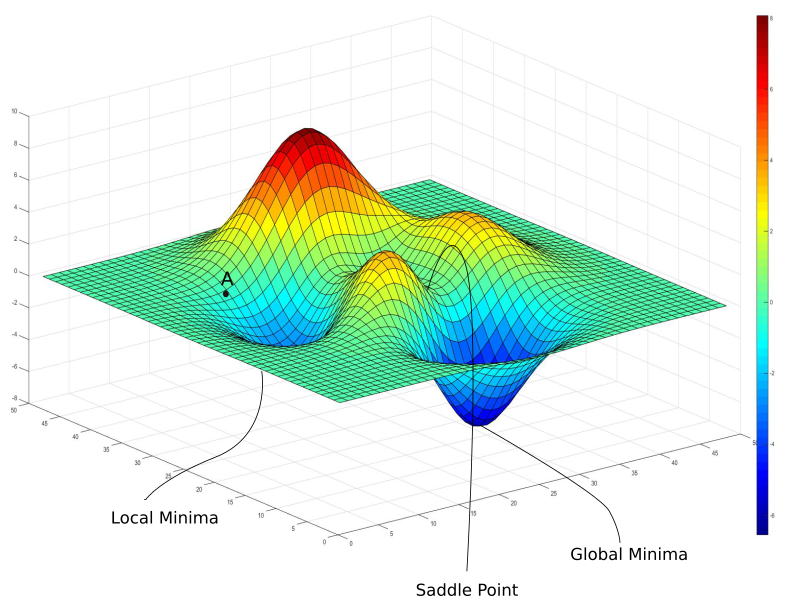
\includegraphics[width=0.8\textwidth]{vallata}
\caption{Grafico di una loss function con due sole variabili}
\label{vallata}
\end{figure}

Minimizzare la loss function significa individuare un\footnote{l'esistenza di un minimo globale non ne implica l'unicità: possono esserci più minimi locali di $L$ di uguale valore, che potrebbero anche essere minimi globali di $L$.} suo punto di minimo globale, partendo da un punto casuale e seguendo la direzione opposta a quella del \textbf{gradiente di $L(\mathcal{W})$} (la "discesa" verso il punto di minimo è cioè "guidata" dal gradiente di $L$). Il gradiente di $L(\mathcal{W})$ si indica con $\nabla L(\mathcal{W})$.

Il metodo della \textbf{discesa stocastica del gradiente} (\textit{stochastic gradient descent}, SGD), usato per minimizzare la loss function, prevede di calcolare $L$ non più sull'intero training set ma su un suo sottoinsieme detto \textbf{\textit{mini-batch}}, costituito da un numero ridotto di esempi (valori tipici sono 16, 32, 64, 128 o 256). La $L^{*}$ così ottenuta è ovviamente una approssimazione della $L$, tanto più buona quanto più il mini-batch è grande e "vario" (cioè quanto più gli esempi di ogni classe sono proporzionalmente presenti nel mini-batch). L'addestramento prevede allora che un'epoca di addestramento sia in realtà divisa in $\frac{|X|}{|\text{mini-batch}|}$ iterazioni per epoca, in ognuna delle quali si presenta alla rete un mini-batch, si calcola la relativa $L^{*(i)}(\mathcal{W})$, si calcola il gradiente $\nabla L^{*(i)}(\mathcal{W})$ e si effettua un "salto" $\Delta \mathcal{W}^{(i)}$ da un punto (calcolato all'iterazione precedente in base alla $L^{*(i-1)}$) ad un altro del dominio di $L^{*(i)}$. Il salto $\Delta \mathcal{W}^{(i)}$ è un vettore di $|\mathcal{W}|$ componenti, ciascuna delle quali rappresenta l'aggiornamento $\Delta w^{(i)}$ del parametro $w^{(i)}$ ed è dato da (supponendo $w^{(i)}$ appartenente all'$l$-esimo layer):
\[
\Delta w^{(i)}=-\text{glr}\times \text{llr}_l\times \frac{\partial L^{*(i)}}{\partial w^{(i)}}
\]
dove con glr = \textbf{learning rate globale} e $\text{llr}_l$ = \textbf{learning rate locale} dell'$l$-esimo layer. Questi sono iperparametri che caratterizzano rispettivamente la rete e i layer addestrabili della rete.\\

Il metodo della discesa del gradiente classico e quello stocastico sono confrontati in figura \ref{fig:gdConfronto}.

\begin{figure}[h!]
\centering
\begin{subfigure}[b]{0.48\textwidth}
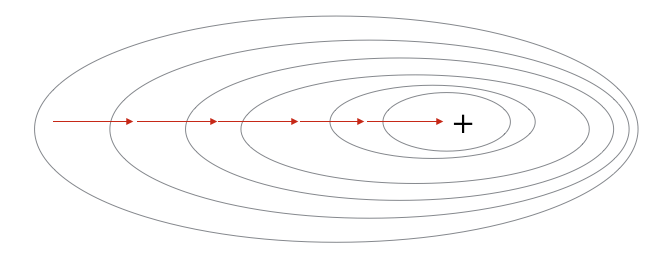
\includegraphics[width=\textwidth]{gd}
\caption{Gradient descent}
\label{fig:gd}
\end{subfigure}
\begin{subfigure}[b]{0.48\textwidth}
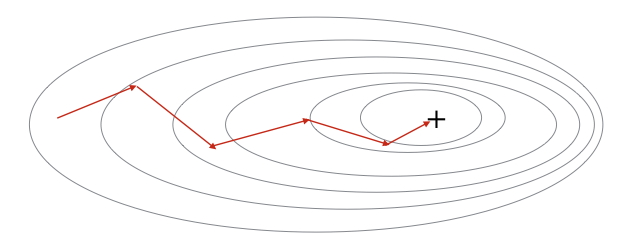
\includegraphics[width=\textwidth]{sgd}
\caption{Stochastic gradient descent}
\label{fig:sgd}
\end{subfigure}
\caption{}
\label{fig:gdConfronto}
\end{figure}

\noindent Alcune importanti osservazioni:

\begin{itemize}

\item La discesa del gradiente converge verso uno dei punti di minimo locale di $L$, non necessariamente in un punto di minimo globale come invece si desidera. Si può dimostrare che la regolarizzazione dei parametri aiuta ad appiattire il grafico di $L$, rendendo i minimi locali e il minimo globale tanto più vicini quanto più i parametri sono "regolarizzati". In queste condizioni, non è un problema il particolare punto di minimo locale in cui la rete converge alla fine dell'addestramento.

\item Nel metodo SGD, ad ogni iterazione il grafico della loss function varia. Se il mini-batch è, come discusso in precedenza, abbastanza grande e vario, le approssimazioni $L^{*(i)}$ sono abbastanza simili tra loro e a $L$ stessa, quindi in questa ipotesi possiamo affermare con buona approssimazione che il punto di minimo verso cui il metodo SGD sta convergendo rimane inalterato ad ogni iterazione.

\item La scelta del learning rate globale e di quelli locali è fondamentale: un learning rate più grande porta ad una convergenza più veloce del metodo SGD verso un punto di minimo locale di $L^{*(i)}$, ma si corre il rischio che dopo molte iterazioni il metodo non sia ancora del tutto "sceso" in uno dei minimi. Infatti per convergere ad un punto di minimo quando si è nelle sue vicinanze c'è bisogno di fare salti di piccola ampiezza verso di esso, a causa della forma a "campana rovesciata" del grafico della funzione attorno ai suoi minimi. Al contrario, un learning rate più piccolo comporta una certa lentezza nella convergenza ma assicura, dopo un sufficiente numero di iterazioni, una loss function più vicina ad un suo minimo. Si può allora mediare tra i due bisogni prevedendo una strategia di \textbf{annealing} (decadimento) del learning rate nel tempo. Ci sono tre tipi comuni di annealing:

\begin{itemize}

\item Step decay: si riduce il learning rate di un certo fattore dopo un certo numero di epoche (ad esempio si dimezza il learning rate ogni 5 epoche)

\item Exponential decay: si riduce il learning rate seguendo la funzione $\text{lr}=\text{lr}_0 e^{-kt}$, dove $\text{lr}_0$ è il learning rate iniziale, $k$ è un iperparametro che regola la velocità di decadimento, $t$ è il "tempo" trascorso (di solito è il numero di iterazioni trascorse o, più comunemente, il numero di epoche trascorse).

\item $1/t$ decay: si riduce il learning rate seguendo la funzione $\text{lr}=\text{lr}_0 /(1+kt)$; le variabili che compaiono hanno lo stesso significato del punto precedente.

\end{itemize}

\end{itemize}
 
\subsubsection{SGD with momentum}
Una variante frequentemente adoperata del metodo SGD è il metodo di \textbf{discesa stocastica del gradiente con momento} (\textit{stochastic gradient descent with momentum}, SGDM).
Il \textbf{momento} è un termine dipendente dalle iterazioni precedenti, che viene sommato al gradiente nel tentativo di regolarizzare il movimento nello spazio dei parametri.
La differenza con l'SGD classico consiste nel salto da compiere nel dominio di $L^{*(i)}$: ad ogni iterazione il salto $\Delta \mathcal{W}^{(i)}$ ha componente (lungo la dimensione del generico parametro $w^{(i)}$ appartenente all'$l$-esimo layer):
\[
\Delta w^{(i)}=-\text{glr}\times \text{llr}_l\times \frac{\partial L^{*(i)}}{\partial w^{(i)}}+\underbrace{\mu\times\Delta w^{(i-1)}}_{\text{momento}}
\]

L'effetto del momento è simile a quello che in fisica ha la quantità di moto (in inglese \textit{momentum}) nello spostamento di un oggetto: così come una forza che sposta un oggetto in una direzione gli fa acquistare velocità (quindi quantità di moto) in quella direzione, l'opposto del gradiente della loss function fa acquistare "velocità" nello spostamento verso il punto di minimo di $L^{*(i)}$, cosicché se il gradiente ha una certa stabilità nella sua direzione per più iterazioni, nell'iterazione successiva il salto avrà una componente lungo quella direzione, a prescindere dal particolare comportamento del gradiente in quella iterazione, "per inerzia".

Questo metodo introduce un ulteriore iperparametro $\mu$ (compreso tra 0 e 1) per controllare l'effetto del momento, ovvero l'importanza dell'iterazione passata: più è grande $\mu$ e più il termine momento assume importanza nell'aggiornamento $\Delta \mathcal{W}^{(i)}$. Un valore empirico per tale parametro è solitamente fissato intorno a 0.9.\\

Il metodo SGDM è visualizzato in fig. \ref{fig:sgdm}

\begin{figure}[h!]
\centering
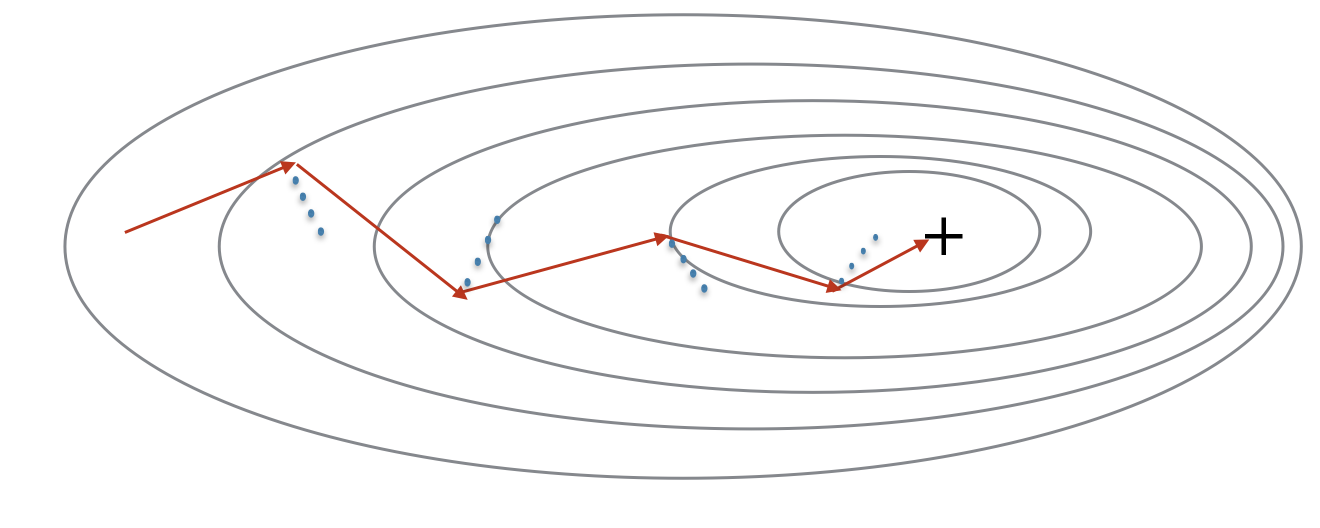
\includegraphics[width=0.5\textwidth]{sgdm}
\caption{Stochastic gradient descent with momentum}
\label{fig:sgdm}
\end{figure}

\subsection{Backpropagation}
\label{backpropagation}
Il calcolo del gradiente della loss function, nell'ambito del metodo SGD e SGDM, avviene analiticamente con il metodo di \textbf{\textit{(error) backpropogation}} (retropropagazione dell'errore). Questo metodo ricorre all'uso ricorsivo della "regola della catena" della derivazione per calcolare le derivate parziali $\frac{\partial L^{*(i)}}{\partial w^{(i)}}$; il calcolo si basa solamente sui valori di output della rete (i punteggi finali per ogni classe). Ad esempio, per una rete neurale standard (con soli strati completamente connessi seguiti ciascuno da una funzione di attivazione $g$) l'algoritmo di backpropagation calcola:
\[
\frac{\partial L^{*(i)}}{\partial w_{ij}^k}=g'(a_j^k)o_i^{k-1}\sum_{l=1}^{r^{k+1}}w_{jl}^{k+1}\delta_l^{k+1}
\]
dove $w_{ij}^k$ è il peso del collegamento tra il neurone $j$ del layer $k$ e il neurone $i$ del layer $k-1$, $a_i^k$ è il valore dell'attivazione del neurone i del layer $k$ prima dell'applicazione di $g$, $o_i^k$ è l'output del neurone $i$ nel layer $k$, $r_k$ è il numero di nodi nel layer $k$, $\delta_j^k=\frac{\partial L^{*(i)}}{\partial a_j^k}$.\\

Per maggiori approfondimenti sull'algoritmo di backpropagation, si rimanda ad esempio a \cite{dlbook}.

\subsection{Scomparsa ed esplosione del gradiente}
\label{vanishingGradient}
Il problema della \textbf{scomparsa del gradiente} (\textit{vanishing gradient problem}) è un fenomeno che crea difficoltà nell'addestramento delle reti neurali profonde tramite SGD/SGDM e backpropagation.

Una delle principali cause è la presenza di funzioni di attivazione non lineari classiche, come la tangente iperbolica o la sigmoide, che hanno gradiente a valori nell'intervallo $(0,1)$.
Poiché nell'algoritmo di retropropagazione i gradienti ai vari livelli vengono moltiplicati tramite la regola della catena, il prodotto di $n$ numeri in $(0,1)$ decresce esponenzialmente rispetto alla profondità $n$ della rete, rendendo quasi nullo l'aggiornamento dei parametri negli strati più bassi della rete.

Inoltre, valori grandi (in valore assoluto) passati alle funzioni di attivazione citate si trovano in zone del dominio delle funzioni dette "di saturazione", in cui la derivata è prossima allo 0. Ciò acuisce il problema numerico sopracitato.\\

Quando invece il gradiente delle funzioni di attivazione può assumere valori elevati, un problema analogo che può manifestarsi è quello dell'\textbf{esplosione del gradiente} (\textit{exploding gradient problem}).\\

Come si vedrà nei paragrafi dedicati alla descrizione delle reti neurali convoluzionali utilizzate negli esperimenti, il problema della scomparsa e dell'esplosione del gradiente viene risolto tipicamente usando funzioni di attivazioni ReLU e, dall'avvento di ResNet, le cosiddette \textit{skip connections} (par. \ref{residualBlock}).

\section{Transfer Learning}
\label{transferLearning}
Nella pratica, poche persone costruiscono e addestrano reti neurali da zero con inizializzazione casuale dei parametri (\textit{from scratch}) per risolvere un task, poiché è relativamente raro disporre di un training set di dimensioni adeguate. Un'alternativa è riutilizzare una rete addestrata su un dataset molto grande (es. ImageNet, par. \ref{imagenet}) e ri-addestrandola per risolvere il task di interesse, con dovuti accorgimenti che saranno spiegati nel seguito.
Questa tecnica si chiama \textbf{\textit{transfer learning}}.

Per esempio, possiamo riutilizzare una rete che è stata addestrata a classificare gatti e cani ri-addestrandola per riconoscere invece formiche e vespe. Se il dataset utilizzato nel task originale è più grande di quello disponibile per il secondo task, il transfer learning è in grado di aumentare significativamente la capacità di generalizzazione (e quindi le performance) del classificatore.
Il motivo per cui il transfer learning funziona è che molte categorie condividono alcune caratteristiche di basso livello come bordi, forme geometriche, cambi nell'intensità dell'illuminazione ecc \cite{howtransferable}. In generale, quindi, il transfer learning è una forma di representation learning usata con successo quando esistono concetti comuni ad un basso livello di astrazione tra le categorie del primo e del secondo task.

L'applicazione del transfer learning è schematizzata in fig. \ref{fig:transferLearning}

\begin{figure}[h!]
\centering
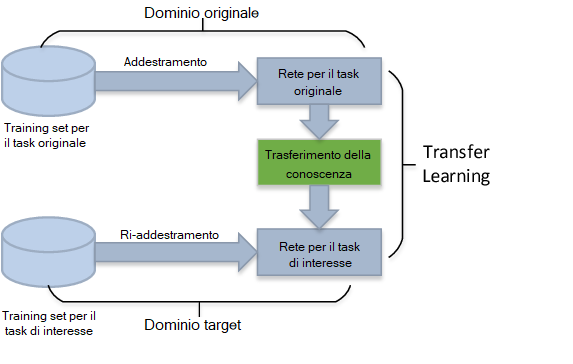
\includegraphics[width=0.75\textwidth]{transferLearning}
\caption{Schema di applicazione del transfer learning}
\label{fig:transferLearning}
\end{figure}

Il metodo del transfer learning per l'addestramento di un modello di classificazione consiste nei seguenti passi:
\begin{enumerate}
\item Selezione di una rete pre-addestrata

Al giorno d'oggi è estremamente facile reperire reti pre-addestrate: molte istituzioni di ricerca rendono pubblici modelli addestrati su dataset ampi e complessi (es. ImageNet), che possono essere riutilizzati per la tecnica del transfer learning.

\item (Opzionale) Azzerare i learning rate dei layer addestrabili più bassi

Questo passaggio ha l'obiettivo di "congelare" l'apprendimento dei layer che rappresentano le feature di livello più basso delle immagini, cioè inibire modifiche ai parametri addestrabili di quei layer. Generalmente, più piccolo è il training set a disposizione per il task di interesse e più layer iniziali andrebbero congelati; con pochi dati, infatti, c'è il rischio di overfitting della rete, problema aggirabile limitando la capacità di rappresentazione del modello che si vuole addestrare.

\item (Opzionale) Aumentare i learning rate dei layer addestrabili finali

Questo passaggio ha l'obiettivo di velocizzare l'apprendimento dei layer che rappresentano le feature di livello più alto delle immagini, al fine di migliorare la capacità della rete di mettere insieme le feature estratte nei livelli intermedi per effettuare la predizione.

\item Rimpiazzare il layer di classificazione finale

Si rimpiazza questo layer per cambiare le classi da predire: non più le classi del task originale (es. le mille classi di ImageNet) ma quelle del task di interesse (es. 'Pinna' e 'No Pinna').

\item Addestrare la rete.

La rete pre-addestrata, opzionalmente modificata a livello dei suoi learning rate locali, è usata come punto di partenza per il nuovo addestramento, che la porterà ad adattarsi al task di interesse.

\item Misurare le prestazioni del modello "trasferito" con un test set.

\end{enumerate}

Il transfer learning è utilizzato nel presente lavoro per adattare quattro modelli pre-addestrati al task di classificazione delle pinne dorsali dei cetacei (cap. \ref{esperimenti}).

\section{Ensemble learning}
\label{ensemble}
Al fine di migliorare l'accuratezza della classificazione, spesso si ricorre ad una strategia conosciuta come \textbf{apprendimento ensemble} (\textit{ensemble learning}). L'idea chiave è quella di creare un insieme (\textit{ensemble}) di classificatori di immagini, ciascuno dei quali è chiamato a "votare" circa l'esito della predizione; a seconda dello "schema di consenso" (\textit{consensus scheme}) scelto per l'ensemble, cioè a seconda di quanto peso assume ciascun voto nella classificazione finale, l'output complessivo sarà la classe che avrà ricevuto "democraticamente" il maggior consenso. La fig. \ref{fig:ensembleSchema} mostra lo schema di funzionamento di un classificatore ensemble.
\vspace{3mm}

\begin{figure}[h]
\centering
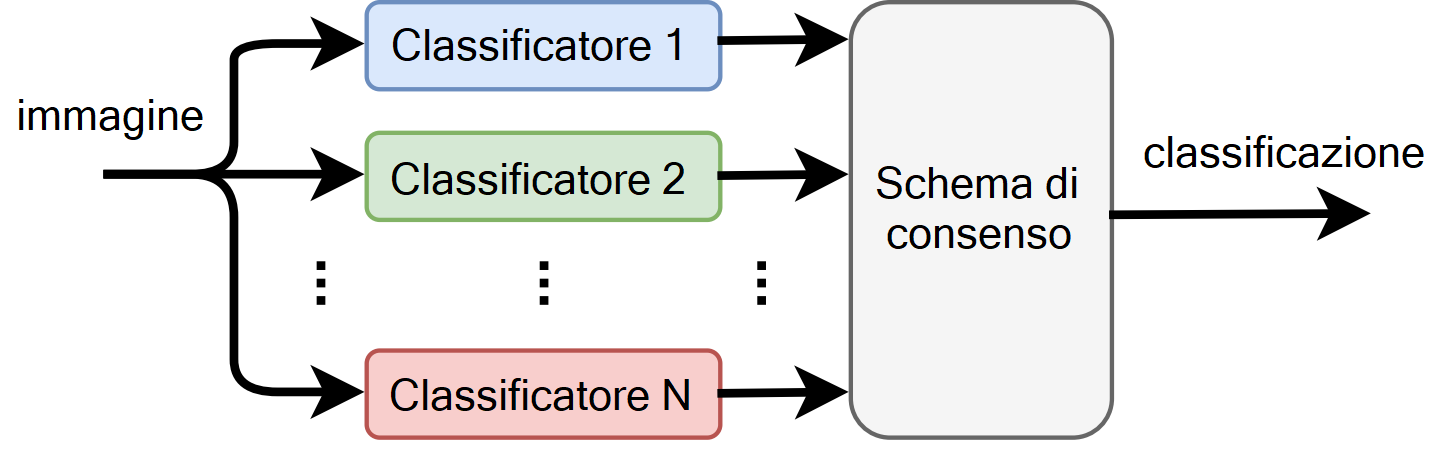
\includegraphics[width=0.9\textwidth]{ensembleSchema}
\caption{Schema di un classificatore ensemble}
\label{fig:ensembleSchema}
\end{figure}

Gli schemi di consenso più utilizzati sono i seguenti:

\begin{itemize}
\item \textbf{\textit{Hard major voting}} (HMV): la classe predetta per l'immagine in input è quella che ha ricevuto il maggior numero di "voti" (predizioni) da parte delle reti dell'ensemble.

\item \textbf{\textit{Soft major voting}} (SVM): la classe predetta per l'immagine in input è quella la cui probabilità di classificazione media (cioè la media delle probabilità softmax relative a quella classe attribuite dalle reti dell'ensemble) è la più grande.
\end{itemize}

L'efficacia dei metodi ensemble è dovuta al fatto che, solitamente, differenti modelli addestrati per risolvere uno stesso problema di classificazione non faranno tutti gli stessi errori sul \textit{test set} (gli errori si possono cioè considerare, in buona sostanza, incorrelati). Se lo schema di consenso applicato è il \textit{major voting}, si dimostra che l'ensemble di classificatori ha sempre prestazioni migliori o almeno uguali a quelle di ciascuna rete dell'ensemble presa singolarmente; il miglioramento delle prestazioni (specificamente della \textit{test accuracy}\footnote{training/validation/test accuracy = 1 -- training/validation/test error, par. \ref{overfitting}}) è tanto migliore quanto più gli errori commessi dalle reti dell'ensemble sono tra loro incorrelati.\cite{dlbook}\cite{ensembles}\\

Il nuovo classificatore per i ritagli delle pinne, oggetto di sviluppo in questo lavoro di tesi, è in realtà un \textit{ensemble} di tre reti neurali convoluzionali ri-addestrate con la tecnica del \textit{transfer learning} (par. \ref{esperimentoTL}).
\section{AlexNet}\label{alexnet}
AlexNet è una CNN creata tra il 2011 e il 2012 da Alex Krizhevsky, in collaborazione con Ilya Sutskever e Geoffrey Hinton \cite{alexnet}. La vittoria di AlexNet nella \textit{ImageNet Large Scale Visual Recognition Challenge (ILSVRC)} (par. \ref{imagenet})\footnote{\url{http://image-net.org/challenges/LSVRC/2012/results}}, ottenuta con un netto distacco nei confronti degli altri concorrenti, ha segnato l'inizio dell'enorme successo ottenuto dalle reti neurali profonde in svariati domini di applicazione \cite{historydl}.

Il risultato principale di AlexNet, così come dichiarato dai suoi creatori nell'articolo originale, è il fatto che la profondità del modello è stato essenziale per conferirgli prestazioni così alte. Il costo computazionale dell'addestramento di AlexNet, reso oneroso appunto dalla profondità del modello (e quindi dal grande numero di parametri - circa 62.3 milioni), è stato affrontato con l'impiego di schede grafiche (GPU), che cominciavano in quegli anni a raggiungere notevoli potenze di calcolo.

\subsection{Architettura di AlexNet}
L'architettura di AlexNet è riportata schematicamente nella figura \ref{arc_alexnet} e con maggiore dettaglio in tabella \ref{tab_arc_alexnet}.
La rete accetta in input immagini $227\times 227$. Essa si compone di otto layer con parametri - cinque convoluzionali e tre completamente connessi. L'output dell'ultimo layer completamente connesso passa per un softmax layer a 1000 vie, il quale fornisce la distribuzione di probabilità per le 1000 classi del dataset ImageNet.

Tra ognuno degli otto strati parametrizzati sono interposti alcuni strati intermedi: ReLU layer, Local Response Normalization layer, Max Pooling layer, Dropout layer. Ognuno di questi sarà analizzato in maggiore dettaglio nei paragrafi successivi.

\begin{figure}[h]
\centering
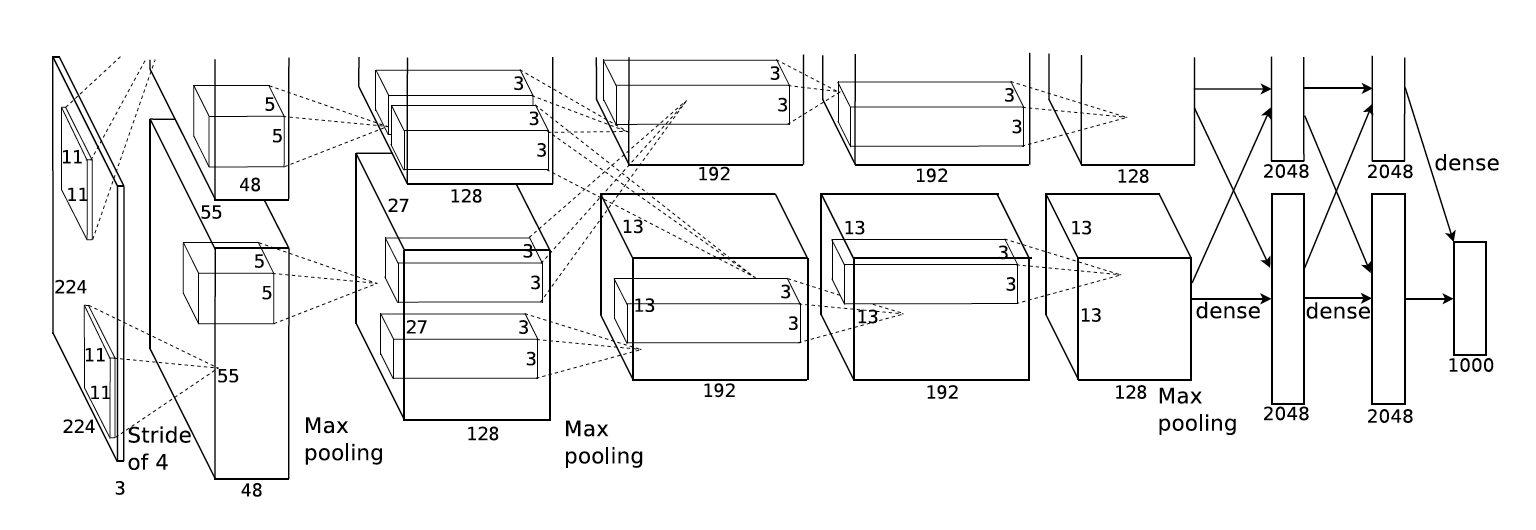
\includegraphics[width=\textwidth ,keepaspectratio]{arc_alexnet}
\caption{Architettura originale di AlexNet \cite{alexnet}}
\label{arc_alexnet}
\end{figure}

Come si evince dalla figura \ref{arc_alexnet}, la rete è composta da due "\textit{pipeline}" parallele. Si scelse infatti di "estendere" la rete su due GPU NVIDIA\textsuperscript{\textregistered} GeForce\textsuperscript{\textregistered} GTX 580 3GB in fase di training, per raddoppiare la memoria massima disponibile (6GB in totale) per conservare la rete e i suoi parametri.

Queste GPU si prestano bene a lavorare in parallelo, poiché possono leggere e scrivere l'una sull'altra direttamente, senza passare dalla memoria della macchina host. Lo schema di parallelizzazione a due vie prevede che su ogni GPU risieda la metà dei kernel (o dei neuroni) di ciascuno strato parametrizzato. Le GPU possono comunicare tra loro solo in certi strati. In particolare, i kernel del layer convoluzionale 1 e 3 hanno in input l'intero output volume rispettivamente del layer di input e del layer convoluzionale 2, mentre i kernel dei rimanenti strati convoluzionali hanno in input la sola metà dell'output volume presente nella stessa GPU (\textit{grouped convolution}\footnote{La scelta di questo pattern di connettività fra le due GPU parallele è il risultato di un problema di cross-validation.}.\\

Sono di seguito passate in rassegna le principali scelte architetturali introdotte in AlexNet, ed alcuni dettagli relativi al suo addestramento.

\subsection{Funzione di attivazione ReLU}
Dopo ogni strato parametrizzato, i valori delle attivazioni sono passati alla funzione attivatrice "rettificatore": $f(x)=x^{+}=\max(0,x)$ \cite{nairhinton}. Questa funzione attivatrice non-lineare e non soggetta a saturazione permette un addestramento molto più veloce delle reti convoluzionali profonde, in confronto a funzioni attivatrici fino ad allora più utilizzate come la funzione sigmoidea $f(x)=(1+\exp^{-x})^{-1}$ e la funzione tangente iperbolica $f(x)=\tanh(x)$.

\subsection{Local Response Normalization}
È stato verificato che la seguente normalizzazione delle attivazioni, \textit{Local Response Normalization}, aumenta lievemente la capacità di generalizzazione del modello:

\[b_{x,y}^{i}=a_{x,y}^{i}/\left(k+\alpha \sum_{j=\max(0,i-n/2)}^{\min(N-1,i+n/2)}(a_{x,y}^{j})^{2}\right)^{\beta}\]

dove $a_{x,y}^{i}$ è l'attivazione del neurone ottenuto applicando il kernel $i$-esimo alla posizione $(x,y)$ e applicando in seguito la funzione ReLU, $b_{x,y}^{i}$ l'attivazione normalizzata, $N$ il numero totale di kernel del layer corrente, $k, n, \alpha, \beta$ sono iperparametri; sono stati usati i valori $k=2, n=5, \alpha=10^{-4}, \beta=0.75$.

Questa normalizzazione è adoperata solamente nel primo e nel secondo layer convoluzionale.

\subsection{Overlapping Max Pooling}
La funzione di max pooling in AlexNet è stata caratterizzata dalla scelta di una dimensione del filtro di pooling $3\times 3$ e uno stride di $2$ (producendo quindi una sovrapposizione, o \textit{overlap}, tra le regioni sottoposte a pooling). È stato osservato durante la fase di training che questa funzione di \textit{max pooling con sovrapposizione} ha attenuato lievemente l'\textit{overfitting} della rete.

\subsection{Data Augmentation}
\label{augmentationAlexnet}
Una delle difficoltà che si incontrano spesso quando si vuole addestrare una rete neurale con moltissimi parametri avendo a disposizione un dataset relativamente piccolo è il rischio del sovradattamento (\textit{overfitting}) della rete al training set, che compromette anche seriamente le prestazioni della rete quando le vengono presentati nuovi dati.
In AlexNet l'overfitting è stato ridotto grazie a tecniche di \textit{data augmentation}. In particolare, dopo aver ridimensionato a $256\times 256$ tutte le immagini del training set (scalando prima in modo tale che il lato più corto dell'immagine sia di 256 e in seguito ritagliando un quadrato centrale $256\times 256$ dall'immagine risultante) e sottraendo l'\textit{immagine media} da ciascuna immagine del training set (par. \ref{preprocessing}), il training set così ottenuto è stato "arricchito" con le seguenti immagini:
\begin{itemize}
\item Estrazione casuale di ritagli $224\times 224$\footnote{Le immagini vengono portate a $227\times 227$, cioè la risoluzione di input, attraverso uno \textit{zero-padding} (3 pixel aggiuntivi ai bordi)} dalle immagini
\item Riflessione orizzontale ("a specchio") delle immagini (50\% di probabilità)
\item Somma di un'immagine e le sue componenti principali (PCA)\footnote{L'\textit{analisi delle componenti principali} (PCA, principal component analysis) è una tecnica per la semplificazione dei dati utilizzata nell'ambito della statistica multivariata. In questa sede ci limitiamo a specificare che il suo utilizzo nell'ambito della data augmentation è di evidenziare una importante proprietà delle immagini naturali, e cioè che l'identità di un oggetto è invariante rispetto ai cambi d'intensità e di colori nella sua illuminazione. Si rimanda ad esempio a \cite{PCA} per approfondimenti sulla PCA.}
\end{itemize}

\subsection{Dropout}
\label{dropout}
Un altro modo per ridurre il problema del sovradattamento è l'impiego di tecniche di regolarizzazione dei parametri. AlexNet utilizza la tecnica del \textit{dropout} \cite{dropout}. Questa tecnica consiste nel settare a zero l'attivazione di ciascun neurone di un layer intermedio con probabilità $p$ (AlexNet impiega un dropout con $p=0.5$. I neuroni "azzerati" sono essenzialmente eliminati dalla rete e non contribuiscono né alla propagazione all'indietro del gradiente né al calcolo delle attivazioni nello strato finale (in fase di addestramento). Questa tecnica riduce il \textit{co-adattamento} tra neuroni: ogni neurone non può fare affidamento sulla presenza di altri neuroni, ed è costretto ad apprendere feature utili in congiunzione con diversi sottoinsiemi casuali degli altri neuroni, e non con un solo particolare sottoinsieme, migliorando la generalizzazione su nuovi dati.

In AlexNet, il dropout dei neuroni è utilizzato nei primi due layer completamente connessi. In fase di test, i neuroni di questi due strati sono moltiplicati per 0.5 per tenere conto dell'impiego del dropout in addestramento.

\subsection{Addestramento di AlexNet}
Nella sua forma originale, AlexNet fu addestrato usando la discesa stocastica del gradiente con momento = 0.9, mini-batch = 128 e decadimento dei pesi (weight decay) = 0.0005. Il training set è ovviamente quello di ImageNet.
I pesi in ogni layer sono stati inizializzati con valori aleatori provenienti da una distribuzione gaussiana a media nulla e deviazione standard 0.01. I bias del secondo, quarto e quinto layer convoluzionale e dei tre layer completamente connessi sono stati inizializzati a 1; questa inizializzazione accelera le prime iterazioni dell'addestramento facendo in modo che alle funzioni di attivazione ReLU siano forniti input positivi. Nei rimanenti layer, i bias sono stati inizializzati a 0. Il \textit{learning rate} iniziale è stato 0.01 ed è stato sottoposto ad una strategia di \textit{annealing} che ha previsto la riduzione del learning rate di un fattore 10 ogniqualvolta il \textit{validation error} si stabilizzava (questa regolazione è stata manuale durante l'addestramento). Questa regolazione è avvenuta tre volte durante l'addestramento della rete.

Ulteriori dettagli sulla fase di addestramento di AlexNet possono essere trovati nel paper originale \cite{alexnet}.

\begin{table}[h]
\begin{tabularx}{\textwidth}{@{}llll@{}}
\toprule
N & Layer           & Attivazioni & Parametri \\ \midrule
1  &
INPUT &
$(227\times 227\times 3)$ &
\\ \midrule
2  & CONVOLUTION     & $(55\times 55\times 96)$ &\acapo{Pesi: $(11\times 11\times 3)\times 96$\\Bias: $(96)$} \\
3  & RELU            & --            & --\\
4  & NORMALIZATION   & --            & --\\
5  & MAX POOLING     & $(27\times 27\times 96)$ & -- \\ \midrule
6  & GROUPED CONVOLUTION     & $(27\times 27\times 256)$ & \acapo{Pesi: $(5\times 5\times 48)\times 128\times 2$\\Bias: $(128)\times 2$} \\
7  & RELU            & --            & --          \\
8  & NORMALIZATION   & --            & --          \\
9  & MAX POOLING     & $(13\times 13\times 256)$            &--           \\ \midrule
10 & CONVOLUTION     & $(13\times 13\times 384)$            & \acapo{Pesi: $(3\times 3\times 256)\times 384$\\Bias: $(384)$}          \\
11 & RELU            & --            &   --        \\ \midrule
12 & GROUPED CONVOLUTION     & $(13\times 13\times 384)$ & \acapo{Pesi: $(3\times 3\times 192)\times 192\times 2$\\Bias: $(192)\times 2$}  \\
13 & RELU            & --            &       --    \\ \midrule
14 & GROUPED CONVOLUTION     & $(13\times 13\times 256)$            & \acapo{Pesi: $(3\times 3\times 192)\times 128\times 2$\\Bias: $(128)\times 2$}\\
15 & RELU            & --            &   --        \\
16 & MAX POOLING     &$(6\times 6\times 256)$            &     --      \\ \midrule
17 & FULLY CONNECTED &$4096$& \acapo{Pesi: $4096\times 9216$\\Bias: $4096$} \\ 
18 & RELU            & --            &     --      \\
19 & DROPOUT         & --            &    --       \\ \midrule
20 & FULLY CONNECTED &$4096$&\acapo{Pesi: $4096\times 4096$\\Bias: $4096$}\\
21 & RELU            & --            &   --        \\
22 & DROPOUT         & --            &   --        \\ \midrule
23 & FULLY CONNECTED &$1000$&\acapo{Pesi: $2\times 4096$\\Bias: $2$}\\
24 & SOFTMAX         & --            &    --       \\
25 & CROSS-ENTROPY LOSS  & --            &   --     \\ \bottomrule
\end{tabularx}
\caption{Architettura originale di AlexNet}
\label{tab_arc_alexnet}
\end{table}


a
\section{ResNet}
\label{resnet}
ResNet (abbreviazione di \textit{residual network}) è il nome di un'ampia categoria di reti neurali convoluzionali profonde, caratterizzate dall'utilizzo di particolari blocchi di layer detti \textit{residual blocks}, ideati per risolvere alcuni problemi delle reti molto profonde.
Le reti ResNet propriamente dette sono state introdotte da un gruppo di ricercatori Microsoft nel 2015 nel paper \cite{resnet}. Presentate nell'edizione del 2015 della \textit{ILSVRC}\footnote{\url{http://image-net.org/challenges/LSVRC/2015/results}} e risultate vincitrici con uno strabiliante errore \textit{top-5} su dataset ImageNet 3.57\% (più basso di quello umano, stimato a 5\%), queste reti sono considerate tutt'oggi lo stato dell'arte nell'ambito delle reti neurali convoluzionali profonde.\\

Nell'ambito dei problemi di visione artificiale proposti nella ILSVRC, in quegli anni cominciava ad essere evidente (\cite{googlenet},\cite{verydeep}) che la profondità delle reti neurali era di fondamentale importanza per il miglioramento delle prestazioni delle reti su dataset di grandi dimensioni, quali il database ImageNet (par. \ref{imagenet}).
L'ovvia conseguenza di questa osservazione è stato il tentativo di aumentare progressivamente il numero di layer delle reti neurali, rendendole sempre più profonde e complesse, con l'aggravarsi di ostacoli già noti (quali ad esempio il problema della scomparsa del gradiente, par. \ref{vanishingGradient}) e il presentarsi di nuovi (un problema di degradazione esposto per la prima volta in \cite{highway}, e descritto nel seguito):
ResNet nasce per dare soluzione a questi problemi:

\begin{itemize}

\item Il problema della scomparsa e dell'esplosione del gradiente è attenuato da un insieme di strategie già messe in campo in precedenza, su tutte la \textit{batch normalization} (par. \ref{batchNormalization}) introdotta dal team dei creatori di GoogLeNet \cite{batchNorm}.

\item Quando una rete molto profonda comincia a convergere verso un minimo della funzione costo (in fase di addestramento), si presenta un problema di degradazione: al crescere della profondità della rete la sua \textit{training accuracy} tende a saturarsi e in seguito prende a degradarsi rapidamente, come mostrato in fig. \ref{fig:degradation}.

\begin{figure}[h!]
\centering
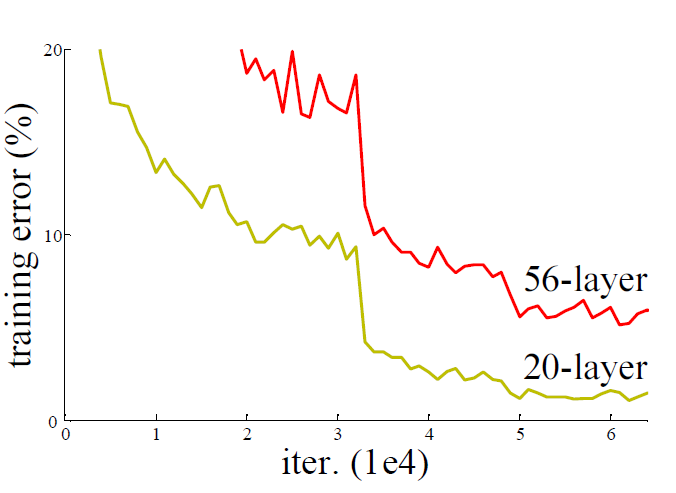
\includegraphics[width=0.5\textwidth]{degradation.png}
\caption{Problema di degradazione della \textit{training accuracy} su CNN "standard" da 20 e 56 layer rispettivamente. La rete più profonda ha un \textit{training error} più alto. \cite{resnet} per più dettagli.}
\label{fig:degradation}
\end{figure}

È un problema inaspettato e diverso rispetto all'\textit{overfitting} (che interessa solamente il valore della \textit{validation accuracy}) e indica che la difficoltà nell'ottimizzare una rete convoluzionale "standard" cresce con la sua profondità. ResNet aggira questo problema con l'introduzione dei \textit{residual blocks} (par. \ref{residualBlock})

\end{itemize}

\subsection{\textit{Batch Normalization}}
\label{batchNormalization}
La \textit{Batch Normalization} è il nome di una tecnica introdotta dal team di GoogLeNet e ad oggi ampiamente utilizzata che permette un addestramento più veloce e stabile delle reti neurali profonde \cite{batchNorm}.

Essa consiste in una normalizzazione delle attivazioni di un certo layer, generalmente prima di passare gli stessi ad un'eventuale funzione di attivazione ed in seguito all'eventuale layer successivo.

L'algoritmo per l'applicazione della tecnica è riportato di seguito\\

\begin{adjustwidth}{3em}{0em}

\textbf{Input:} Attivazioni $\mathbf{x}=\{x_1,\dots,x_m\};$\\
\phantom{\textbf{Input:} }Parametri da imparare: $\gamma, \beta$\\
\noindent \textbf{Output:} Attivazioni normalizzate $y_i = BN_{\gamma,\beta}(x_i)\}$

\begin{align}
& \mu_{\mathbf{x}}\leftarrow\frac{1}{m}\sum_{i=1}^m x_i && \text{// media delle attivazioni} \notag\\
& \sigma^2_{\mathbf{x}}\leftarrow\frac{1}{m}\sum_{i=1}^m \left(x_i-\mu_{\mathbf{x}}\right)^2 && \text{// varianza delle attivazioni} \notag\\
& \widehat{x_i}\leftarrow\frac{x_i-\mu_{\mathbf{x}}}{\sqrt{\sigma^2_{\mathbf{x}}+\varepsilon}} && \text{// normalizzazione} \notag\\
& y_i\leftarrow\gamma\widehat{x_i}+\beta\equiv BN_{\gamma,\beta}(x_i)\} && \text{// scale e offset} \notag
\label{eq:batchNorm}
\end{align}

\end{adjustwidth}

I parametri $\gamma$ e $\beta$, chiamati rispettivamente \textit{scale} e \textit{offset}, sono imparati dalla rete in fase di addestramento. La loro funzione è far sì che le attivazioni normalizzate non siano necessariamente a media nulla e varianza unitaria (in modo da poter variare arbitrariamente l'intervallo utilizzato nel dominio della eventuale funzione di attivazione successiva alla normalizzazione).\\

Nonostante sia oggi ampiamente utilizzata, le ragioni dell'efficienza della \textit{batch normalization} sono ancora scarsamente comprese. Ricerche recenti \cite{realBatchNorm} hanno mostrato che ciò che questa tecnica produce non è una riduzione dell'\textit{internal covariate shift} (la variabilità statistica dei mini-batch usati, che ad ogni iterazione causa uno spostamento del punto di minimo della funzione costo), come affermato dagli autori del paper originale \cite{batchNorm}, ma è una "lisciatura" (\textit{smoothing}) della funzione costo, che induce un comportamento più stabile e predicibile dei gradienti, comportando un addestramento più veloce.

In ogni caso, la \textit{batch normalization} si è rivelata efficace per l'attenuazione del problema della scomparsa del gradiente o della sua esplosione; inoltre si è verificato che il suo utilizzo porta anche ad una maggiore regolarizzazione dei parametri dell'apprendimento, migliorando la robustezza all'overfitting.

Questa tecnica ha permesso quindi la progettazione di reti sempre più profonde, ma non elimina tutti i problemi collegati all'estrema profondità dell'architettura (persiste ad esempio il problema di degradazione descritto nel precedente paragrafo).

\subsection{Residual blocks}
\label{residualBlock}
Il principale contributo di ResNet nell'ambito del deep learning è sicuramente l'introduzione dei cosiddetti \textit{residual blocks} e delle \textit{shortcut connections} ("scorciatoie") per risolvere il problema di degradazione in precedenza descritto. In fig. \ref{fig:residualBlock} è mostrato uno schema generale dell'oggetto in esame.

\begin{figure}[h!]
\centering
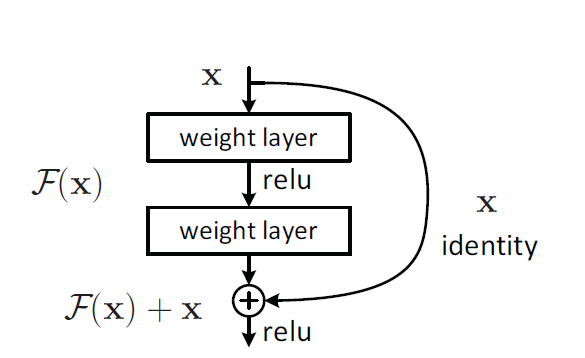
\includegraphics[width=0.6\textwidth]{residualBlock.png}
\caption{\textit{Residual block} con \textit{shortcut identity mapping}. Si noti che i particolari layer di questo blocco sono arbitrari.}
\label{fig:residualBlock}
\end{figure}

Invece di sperare che un dato blocco di layer non lineari contigui impari ad approssimare una certa funzione $\mathcal{H}(\mathbf{x})$ desiderata, si decide di creare una "scorciatoia" (propriamente \textit{shortcut connection}) che connette l'input $\mathbf{x}$ e l'output del blocco (vd. fig. \ref{fig:residualBlock}); in questo modo il blocco deve imparare ad approssimare non più la funzione desiderata $\mathcal{H}(\mathbf{x})$ ma una funzione residuale $\mathcal{F}(\mathbf{x})\coloneqq\mathcal{H}(\mathbf{x})-\mathbf{x}$. In definitiva il blocco addestrato darà in output la funzione $\mathcal{F}(\mathbf{x})+\mathbf{x}$.\\

Per introdurre la motivazione che spinge alla progettazione di questo particolare blocco, facciamo il seguente esperimento.
Consideriamo una generica rete neurale con $n$ layer. Costruiamo una rete neurale con $n+k$ layer che ha come layer iniziali gli $n$ layer della prima rete e i rimanenti $k$ layer approssimano funzioni identità ($\mathcal{F}(\mathbf{x})=\mathbf{x}$). L'esistenza di una seconda rete più profonda della prima ma con le stesse prestazioni indica che una rete più profonda dovrebbe avere un \textit{training error} più basso o almeno uguale a quella meno profonda. Gli esperimenti in \cite{resnet} hanno mostrato tuttavia che non conosciamo nessun algoritmo di ottimizzazione che permetta almeno di eguagliare il \textit{training error} della prima rete addestrando la seconda rete descritta (almeno in un tempo non lungo). Questa è una delle forme in cui si manifesta il \textit{degradation problem} discusso in precedenza.

L'idea dei \textit{residual blocks}, peraltro non nuova e già utilizzata in precedenza (ad es. \cite{highway}), è basata sull'ipotesi degli autori - corroborata dall'esperimento di cui sopra - che le reti neurali abbiano difficoltà ad approssimare attraverso i loro tanti layer non lineari una funzione lineare (come appunto l'identità $\mathcal{f}(\mathbf{x})=\mathbf{x}$); in altre parole, viene ipotizzato che sia più facile per un blocco di layer imparare la funzione residua rispetto alla funzione originale. Ecco perché si decide di fornire direttamente l'input in uscita con una \textit{shortcut connection}, evitando al blocco lo sforzo di dover imparare a mappare un'identità.\\

Le straordinarie prestazioni raggiunte dalle reti ResNet estremamente profonde confermano che l'intuizione degli autori era corretta. Senza aver aggiunto complessità computazionale (escludendo le trascurabili somme dovute alle \textit{shortcut connections}) resta così risolto il problema di degradazione della \textit{training accuracy}.

\subsection{Architettura di ResNet-18}
ResNet-18 è una rete neurale convoluzionale profonda addestrata sul dataset ImageNet (par. \ref{imagenet}). La rete accetta in input immagini $224\times 224$ ed è composta da 18 layer parametrizzati, di cui un layer convoluzionale iniziale con filtro $7\times 7$ (seguito da batch normalization, ReLU e max pooling), altri 16 layer convoluzionali $3\times 3$ raccolti a due a due in 8 \textit{residual blocks} (descritti di seguito) e infine  un layer completamente connesso (preceduto da ReLU e average pooling) dalle cui 1000 attivazioni si calcola la distribuzione di probabilità per le 1000 classi di ImageNet, per mezzo della funzione softmax.
Il particolare \textit{residual block} adoperato in ResNet-18 è del tipo mostrato in figura \ref{fig:residualBlockResnet18}

\begin{figure}[H]
\centering
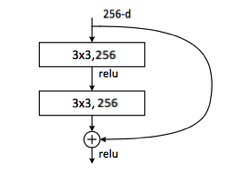
\includegraphics[width=0.4\textwidth]{residualBlockResnet18.png}
\caption{Uno degli otto \textit{residual blocks} di ResNet-18}
\label{fig:residualBlockResnet18}
\end{figure}

Il ramo che ospita i layer non lineari si compone delle seguenti operazioni:

\begin{itemize}
\item Convoluzione $3\times 3$\footnote{il numero di filtri di convoluzione, e quindi la profondità del volume di output, è riportata per ciascun \textit{residual block} in fig. \ref{fig:architetturaResnet18} e in fig. \ref{fig:confrontoResnet}}
\item Batch Normalization
\item ReLU
\item Convoluzione $3\times 3$
\item Batch Normalization
\end{itemize}

Inoltre, il ramo che realizza la \textit{shortcut connection} si compone eventualmente di una convoluzione $1\times 1$ seguita da batch normalization per garantire che il volume di attivazioni che attraversa la "scorciatoia" abbia dimensioni confrontabili con il volume uscente dal ramo che ospita i layer non lineari. Questa eventualità è rappresentata in fig. \ref{fig:architetturaResnet50} con un arco tratteggiato.\\

L'architettura di ResNet-18 è riportata schematicamente nella figura \ref{fig:architetturaResnet18} e in forma tabellare, in confronto con ResNet-50, in fig. \ref{fig:confrontoResnet} nel prossimo sottoparagrafo.

\subsection{Architettura di ResNet-50}
ResNet-50 è una variante più profonda di ResNet-18. Come la sua omologa meno profonda, questa rete accetta in input immagini $224\times 224$; essa è composta da 50 layer parametrizzati, di cui un layer convoluzionale iniziale con filtro $7\times 7$ (seguito da \textit{batch normalization}, ReLU e max pooling), altri 48 layer convoluzionali di varie dimensioni raccolti a gruppi di tre in 16 \textit{residual blocks} (descritti di seguito) e infine  un layer completamente connesso con le usuali 1000 attivazioni.
Il particolare \textit{residual block} adoperato in ResNet-50 è del tipo mostrato in figura \ref{fig:residualBlockResnet50}

\begin{figure}[H]
\centering
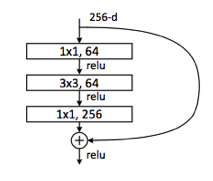
\includegraphics[width=0.4\textwidth]{residualBlockResnet50.png}
\caption{Uno dei sedici \textit{residual blocks} di ResNet-50}
\label{fig:residualBlockResnet50}
\end{figure}

Il ramo che ospita i layer non lineari si compone delle seguenti operazioni:

\begin{itemize}
\item Convoluzione $1\times 1$
\item Batch Normalization
\item ReLU
\item Convoluzione $3\times 3$
\item Batch Normalization
\item ReLU
\item Convoluzione $1\times 1$
\item Batch Normalization
\end{itemize}

Inoltre, il ramo che realizza la \textit{shortcut connection} si compone eventualmente di una convoluzione $1\times 1$ seguita da batch normalization per garantire che il volume di attivazioni che attraversa la "scorciatoia" abbia dimensioni confrontabili con il volume uscente dal ramo che ospita i layer non lineari. Questa eventualità è rappresentata in fig. \ref{fig:architetturaResnet50} con un arco tratteggiato.\\

L'evidente differenza rispetto al \textit{residual block} di ResNet-18 è motivata dalla premura di dover mantenere basso il tempo necessario ad addestrare la rete. Le convoluzioni $3\times 3$ sono computazionalmente costose, pertanto in reti molto profonde non si possono prevedere tutti \textit{residual blocks} ciascuno operante due convoluzioni $3\times 3$. Si decide allora di modificare il \textit{residual block} usato: si decide di operare un'unica convoluzione $3\times 3$ per blocco, preceduta e seguita da una convoluzione $1\times 1$ (par. \ref{1x1conv}) per rispettivamente ridurre e ripristinare la profondità del volume di attivazioni su cui la convoluzione $3\times 3$ lavora, abbassando così il costo computazionale associato all'addestramento di ciascun \textit{residual block}.\\

L'architettura di ResNet-50 è riportata schematicamente nella figura \ref{fig:architetturaResnet50} e in forma tabellare, in confronto con quella di ResNet-18, in fig. \ref{fig:confrontoResnet} seguente.

\begin{figure}[h!]
\centering
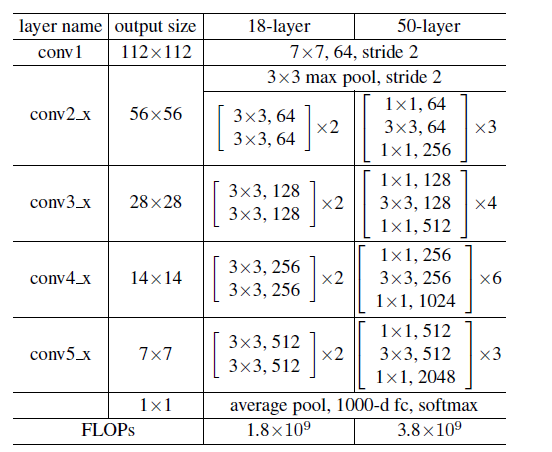
\includegraphics[width=0.8\textwidth, height=\textheight, keepaspectratio]{architetturaResnet.png}
\caption{Le architetture di ResNet-18 e ResNet-50 a confronto}
\label{fig:confrontoResnet}
\end{figure}

\begin{figure}[h]
  \begin{minipage}[b]{0.475\textwidth}
  \centering
    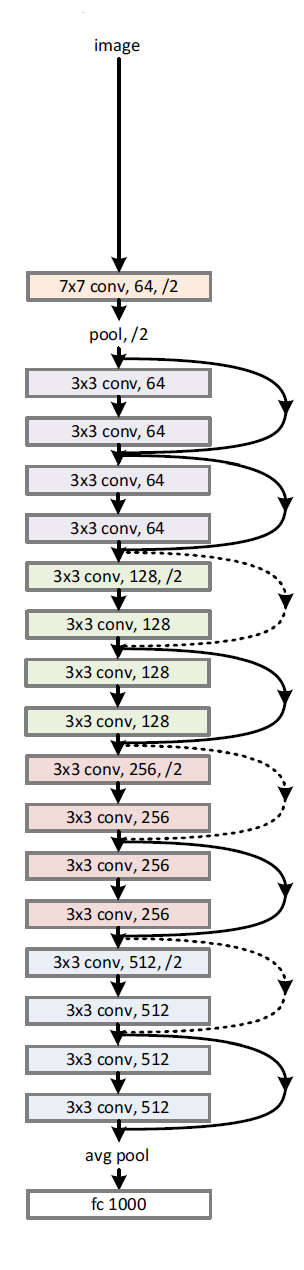
\includegraphics[width=\textwidth, height=\textheight, keepaspectratio]{architetturaResnet18.png}
    \caption{Architettura di ResNet-18}
    \label{fig:architetturaResnet18}
  \end{minipage}
  \hfill
  \begin{minipage}[b]{0.475\textwidth}
  \centering
    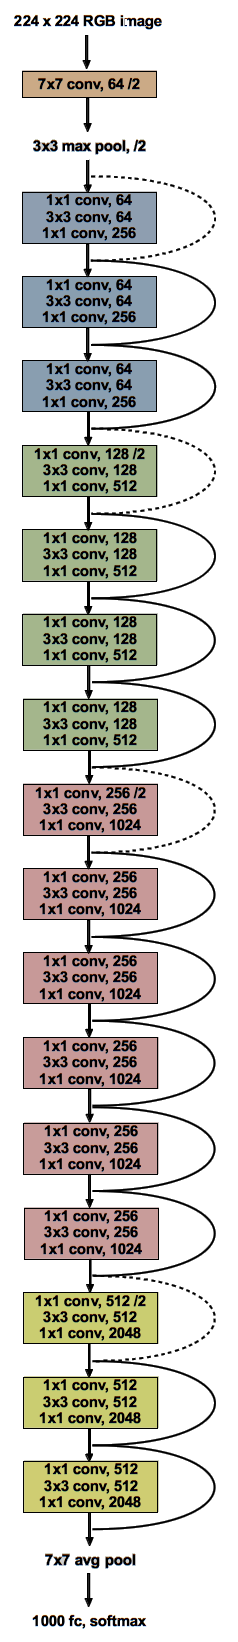
\includegraphics[width=\textwidth, height=\textheight, keepaspectratio]{architetturaResnet50.png}
    \caption{Architettura di ResNet-50}
    \label{fig:architetturaResnet50}
  \end{minipage}
\end{figure}

\subsection{Data Augmentation}
\label{augmentationResnet}
Come d'uso, anche ResNet-18 e ResNet-50 adoperano una strategia di \textit{data augmentation} per ridurre l'overfitting al training set di ImageNet.
Ogni immagine è ridimensionata con il suo lato più corto estratto casualmente dall'intervallo $[256,480]$ e mantenendo l'\textit{aspect ratio}. Viene ritagliata una \textit{patch} (ritaglio) $224\times 224$ casuale dall'immagine così ridimensionata e ad ogni canale della patch viene sottratta la media dei valori R, G e B del dataset ImageNet (similmente ad AlexNet, par. \ref{augmentationAlexnet}). Il ritaglio è eventualmente capovolto orizzontalmente (50\% di probabilità)

\subsection{Addestramento di ResNet-18 e ResNet-50}
Le reti ResNet-18 e ResNet-50 sono state addestrate sul database ImageNet usando la discesa stocastica del gradiente con momento = 0.9, mini-batch = 256 e decadimento dei pesi (\textit{weight decay}) = 0.0001. Il \textit{learning rate} iniziale è 0.1, ed è soggetto ad una strategia di \textit{annealing} che lo riduce di un fattore 10 ogniqualvolta il \textit{training error} si stabilizza. Il numero massimo di iterazioni di addestramento è $6\times 10^5$. I pesi sono inizializzati secondo il metodo descritto in \cite{weightsResnet}, creato dagli stessi autori di ResNet. Dettagli più specifici sulla fase di addestramento di ResNet-18 e ResNet-50 possono essere trovati nel paper originale \cite{resnet}.

%% 3 - Esperimenti e risultati
\chapter{Esperimenti e risultati}\label{esperimenti}
In questo capitolo vengono presentati gli esperimenti condotti e si analizzano i risultati ottenuti.

\section{Descrizione dei dataset utilizzati}
\label{dataset}
Per la conduzione degli esperimenti sono stati adoperati due distinti dataset di immagini, di seguito descritti

\begin{itemize}

\item Il primo, usato per la fase di addestramento delle reti neurali, è una collezione di fotografie di tursiopi (scattate tra luglio 2016 e settembre 2017) e grampi (scattate tra luglio 2013 e agosto 2018) nel \textbf{Golfo di Taranto} (mar Ionio Settentrionale). Le fotografie sono state scattate e messe a disposizione dall'associazione \textit{Jonian Dolphin Conservation} (par. \ref{contesto}). Il dataset contiene immagini acquisite in un'area di 14000 km\textsuperscript{2} percorsa su un catamarano e seguendo rotte prestabilite.
Il dataset acquisito contiene in totale n=10194 immagini, suddivise in cartelle in base alla specie ritratta e ulteriormente ramificate in sottocartelle in base alla data degli scatti.

\item Il secondo, usato per testare le prestazioni dei classificatori binari precedentemente addestrati, consiste in un insieme di fotografie di grampi scattate nel mese di giugno 2018 nei pressi delle \textbf{Isole Azzorre} (Oceano Atlantico settentrionale) dall'associazione \textit{Nova Atlantis Foundation} (par. \ref{contesto}).
Questo dataset contiene in totale n=11290 immagini, anche questa volta suddivise in cartelle in base alla data degli scatti.
\end{itemize}

Entrambi i dataset contengono fotografie con una notevole risoluzione $6000\times 4000$, con occupazione di memoria di circa 10MB per foto e occupazione totale di circa 100GB per dataset. Tuttavia, prendendo visione delle immagini in ciascuno dei due dataset ci si rende subito conto che non tutte contengono pinne dorsali di cetacei: in alcune foto sono totalmente assenti, rendendo lo scatto totalmente privo di contenuto informativo per i biologi.
Anche laddove le pinne sono presenti, esse possono risultare sfocate o di bassa risoluzione se molto lontane, sovrapposte tra due esemplari vicini, disturbate da schizzi d'acqua o riflessi di luce. Infine, in tutte le fotografie sono inevitabilmente ritratti oggetti che non sono informativi ai fini dello studio delle sole pinne dorsali quali barche, persone, uccelli, terraferma (paesaggi), porzioni di cielo, boe, lo specchio d'acqua ma anche parti dei cetacei diversi dalla loro pinna dorsale, quali pinne caudali e laterali, il dorso e la testa degli esemplari. Alcune di queste situazioni sono mostrate in figura \ref{fig:esempiDataset}.

\begin{figure}[h]

  \centering
  
  \begin{subfigure}[b]{\textwidth}
    \includegraphics[width=0.24\textwidth]{t1.jpg}
    \hfill
    \includegraphics[width=0.24\linewidth]{t2.jpg}
    \hfill
    \includegraphics[width=0.24\linewidth]{t3.jpg}
    \hfill
    \includegraphics[width=0.24\linewidth]{t6.jpg}
    \caption{}
  \end{subfigure}
  
  \vspace{5mm}
  
  \begin{subfigure}[b]{\textwidth}
    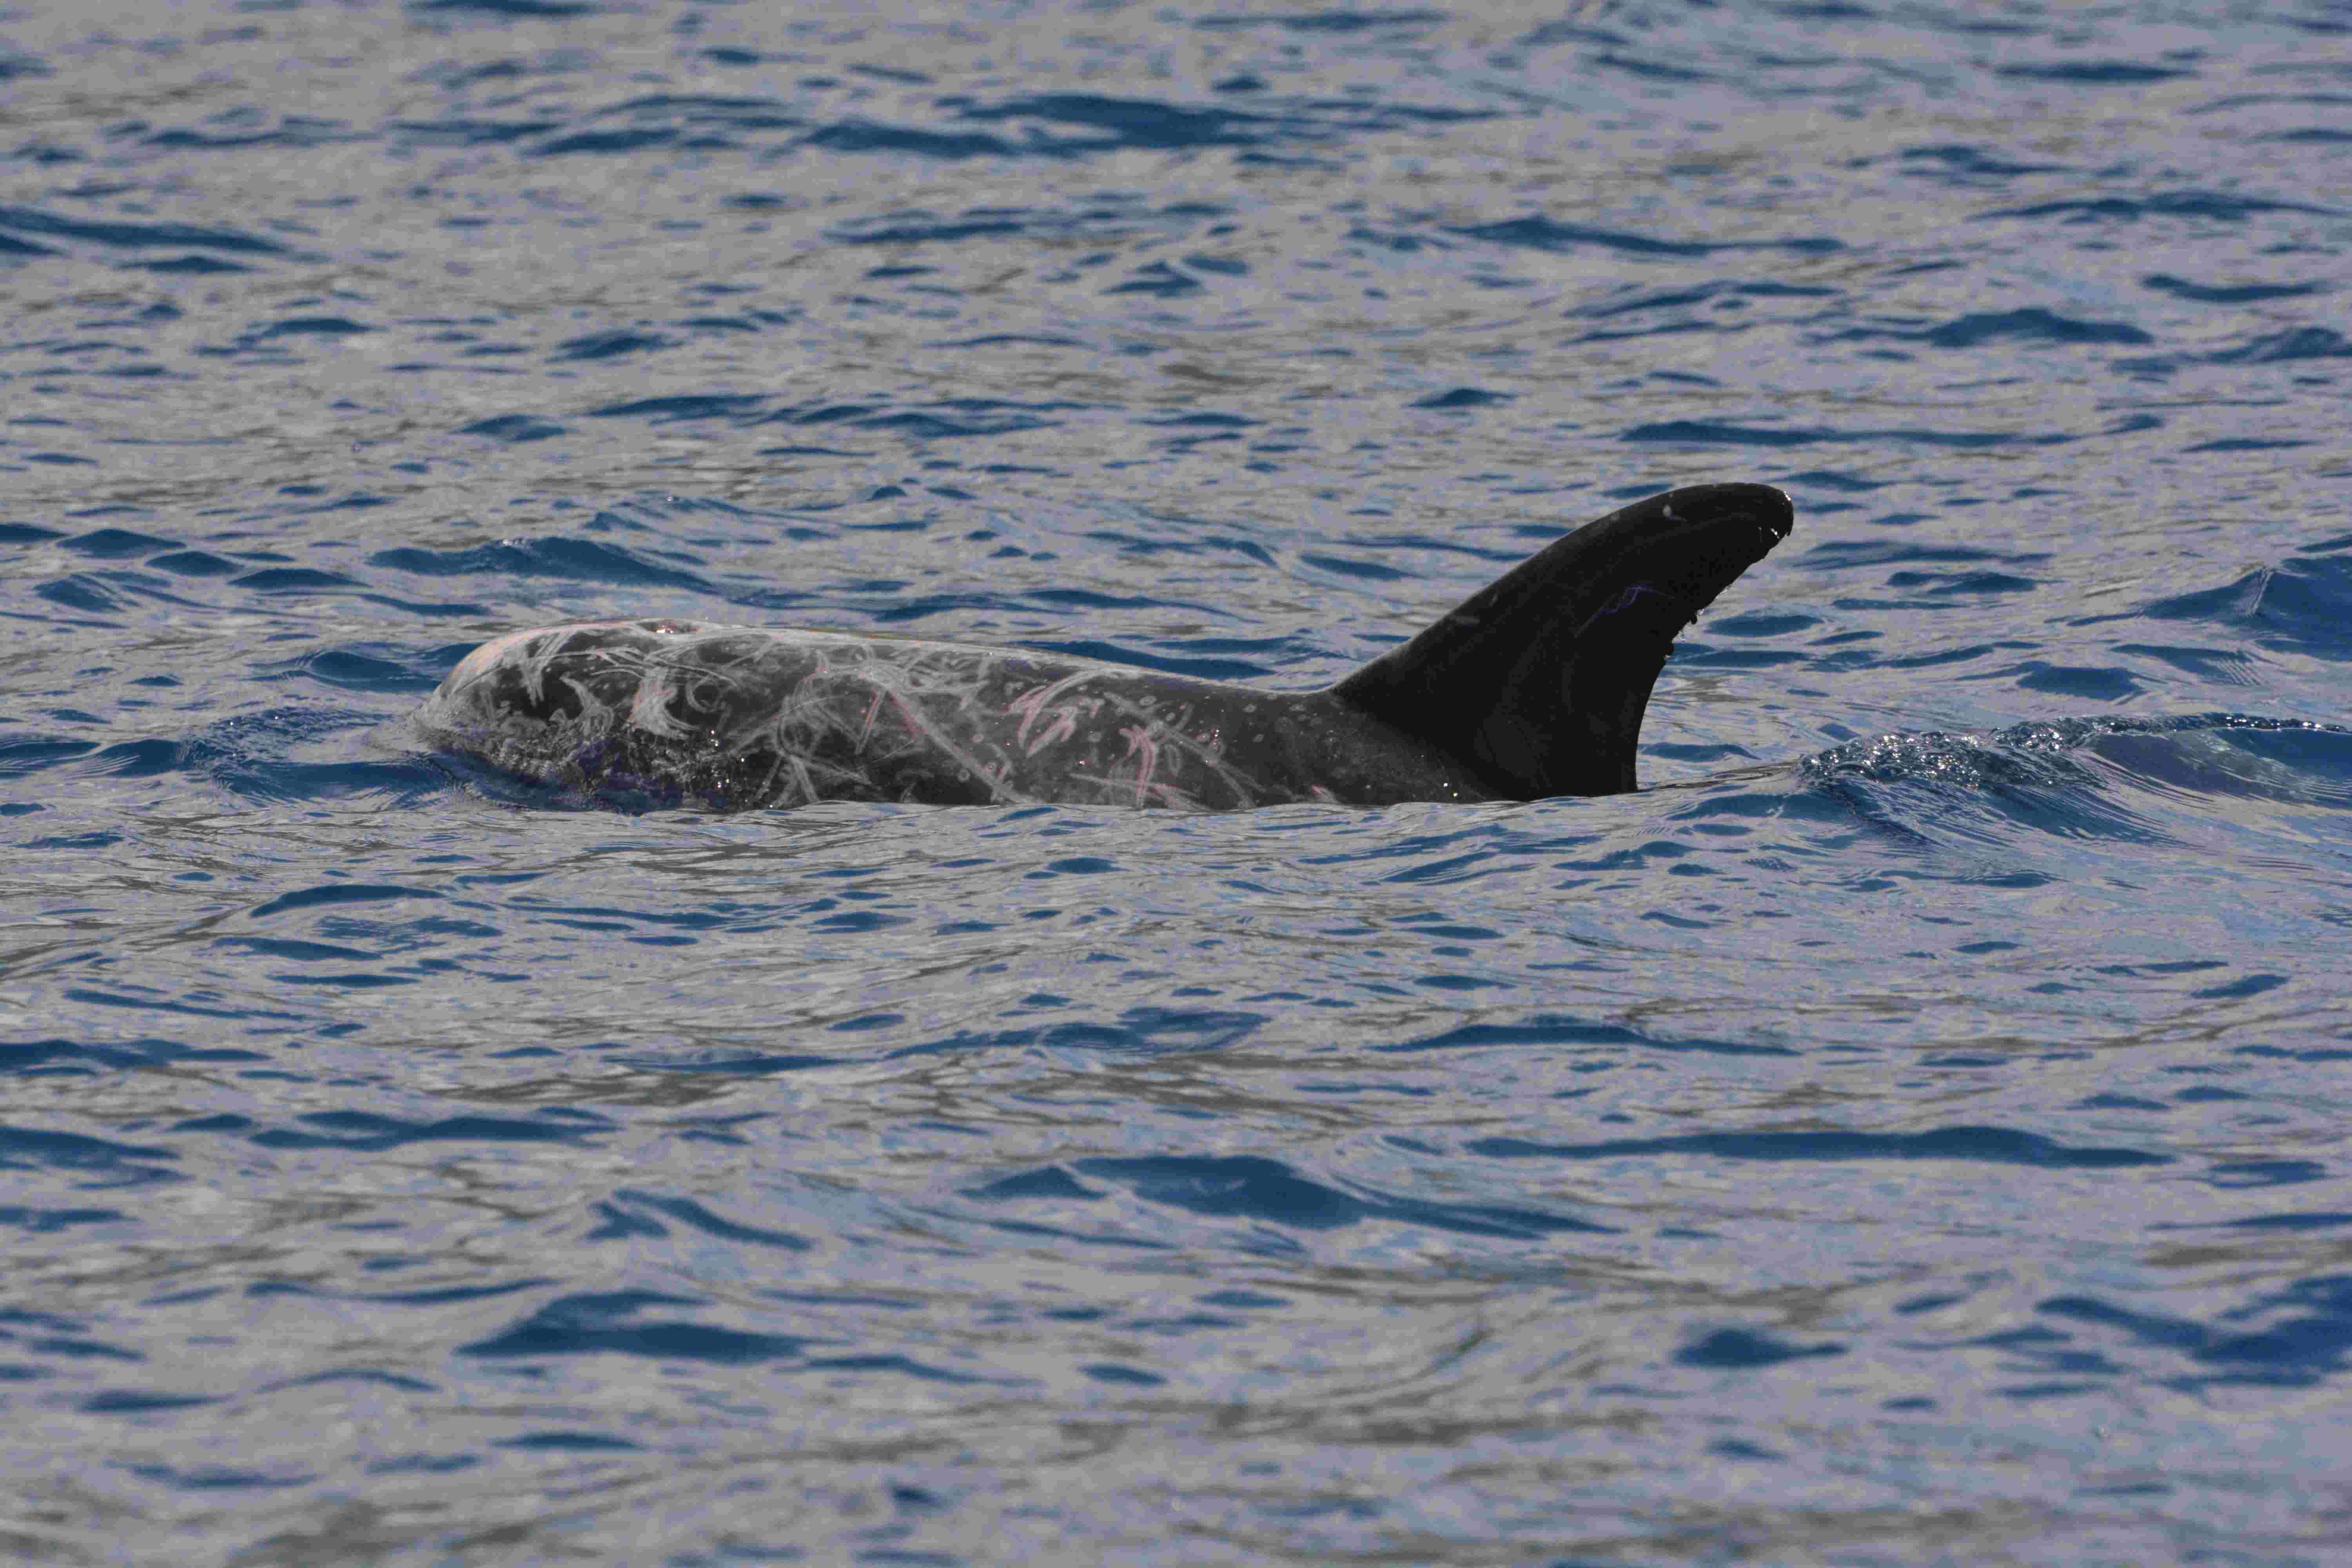
\includegraphics[width=0.24\textwidth]{a1.jpg}
    \hfill
    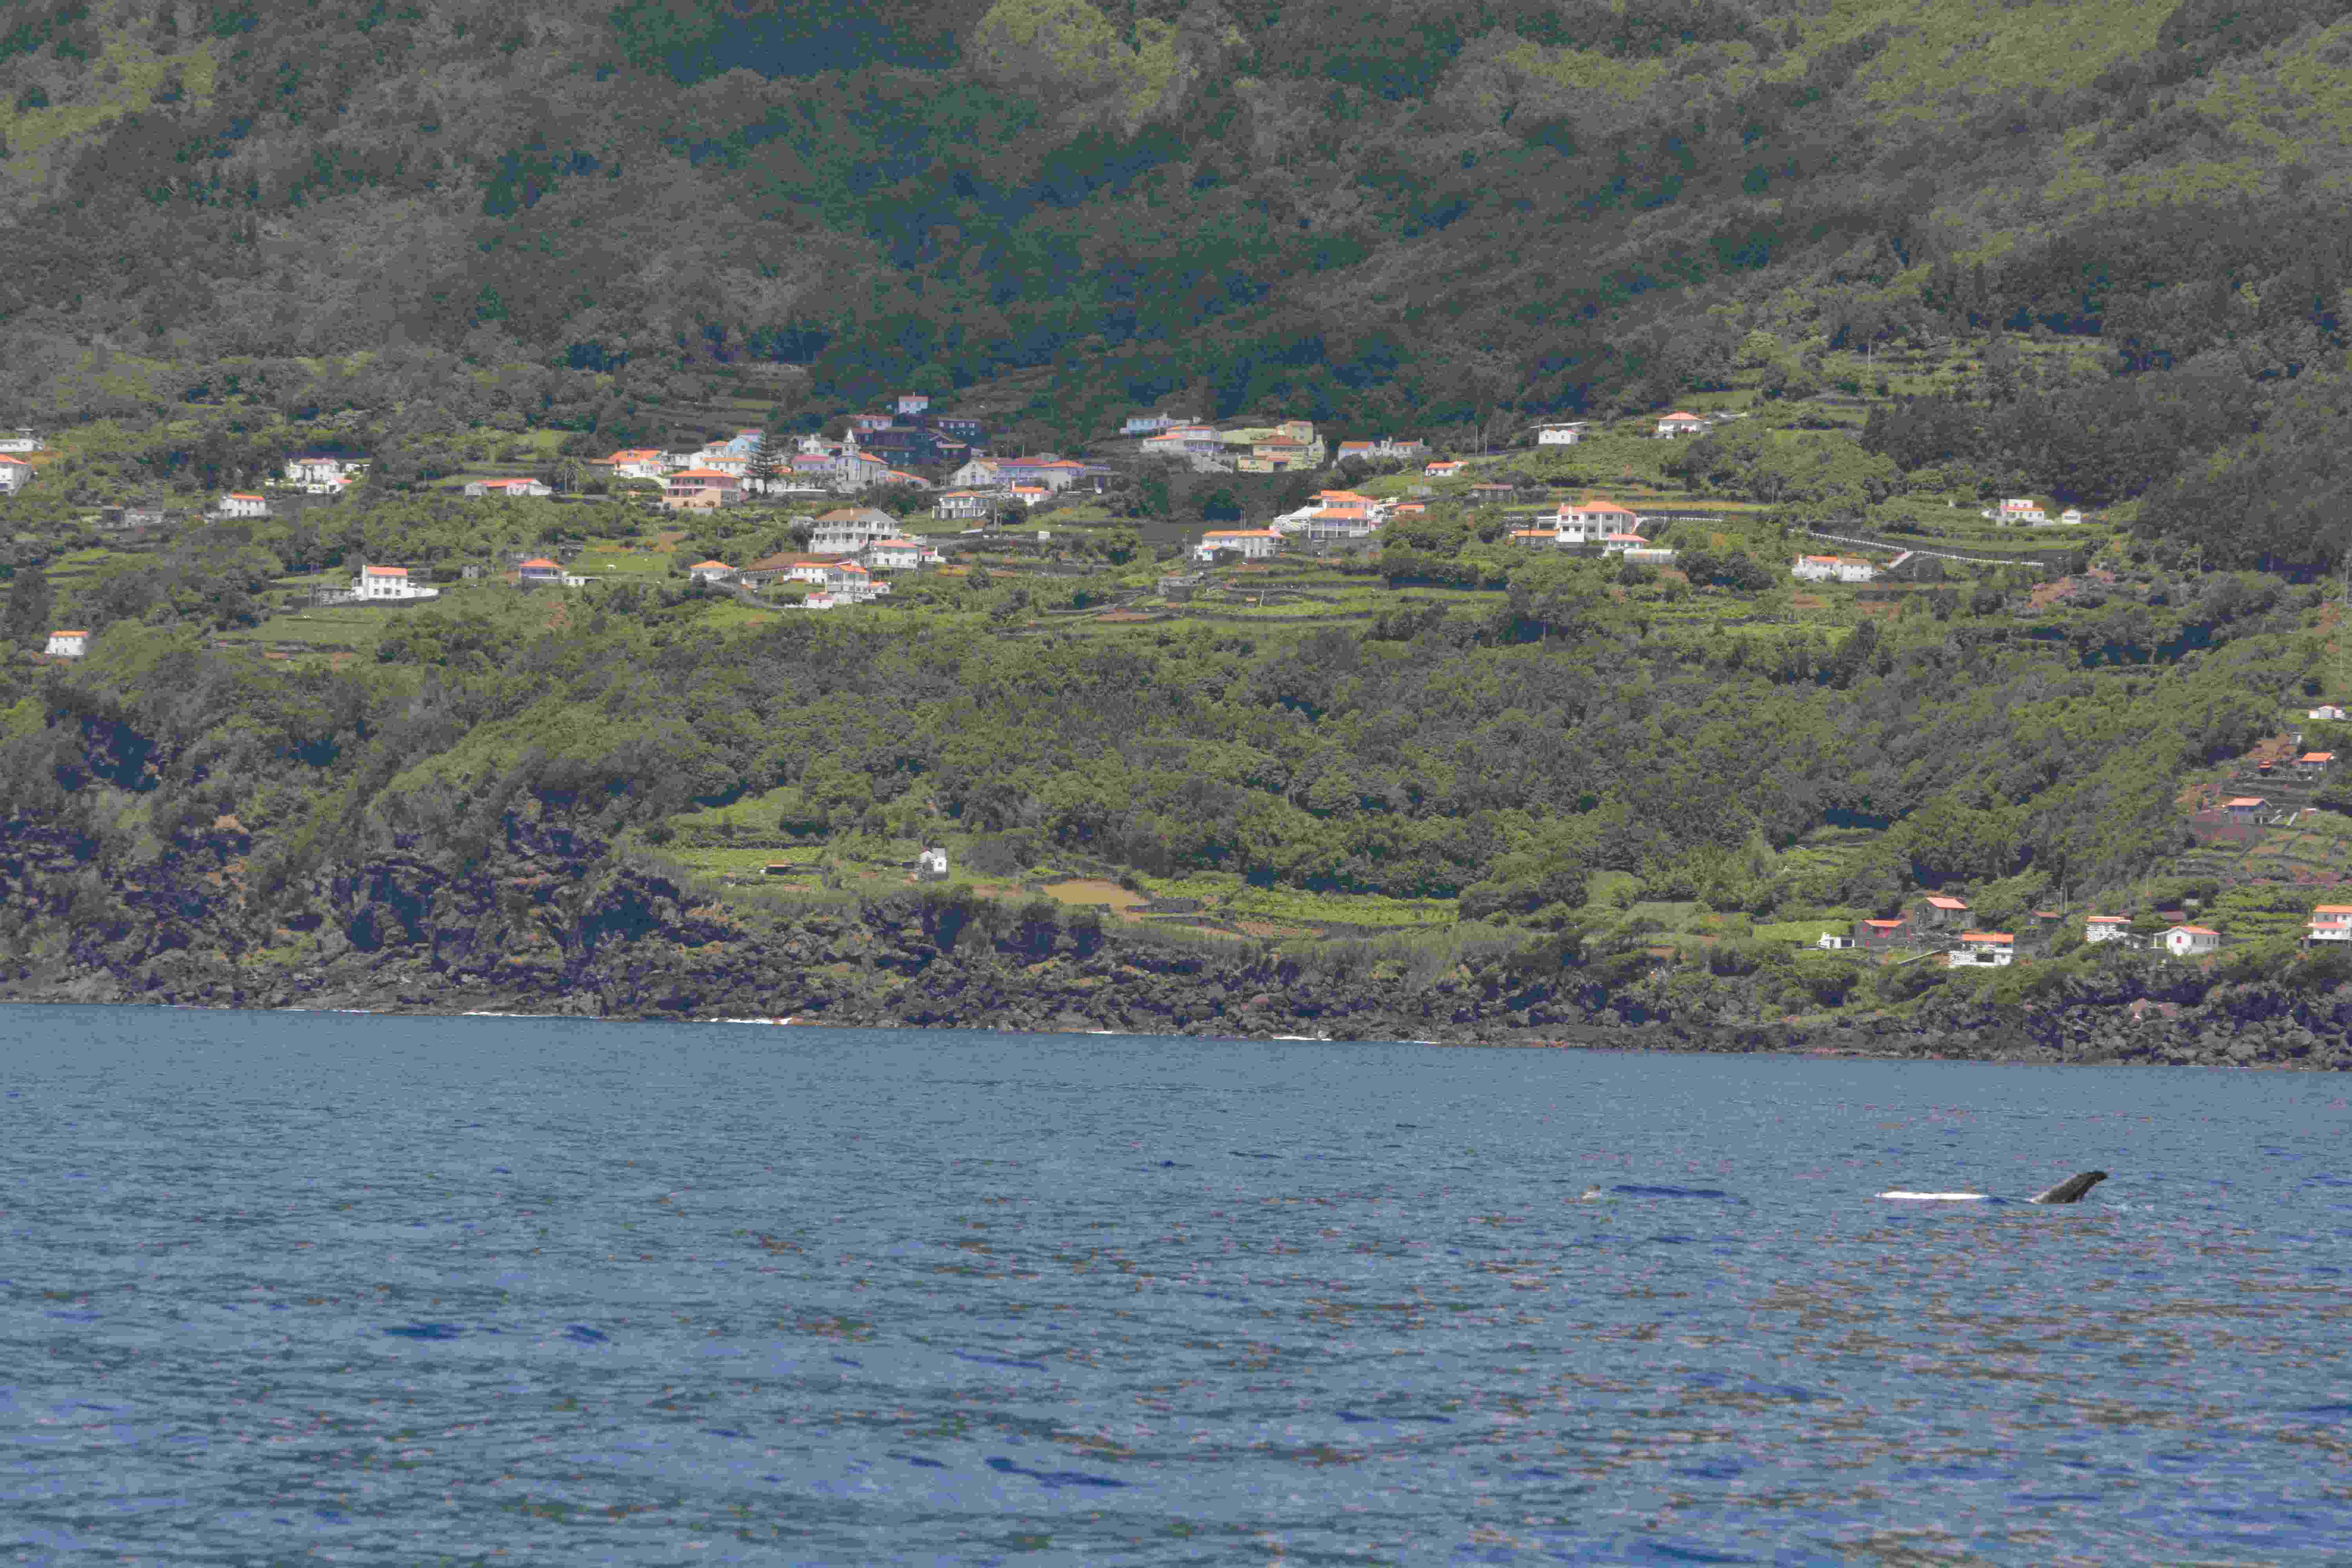
\includegraphics[width=0.24\linewidth]{a2.jpg}
    \hfill
    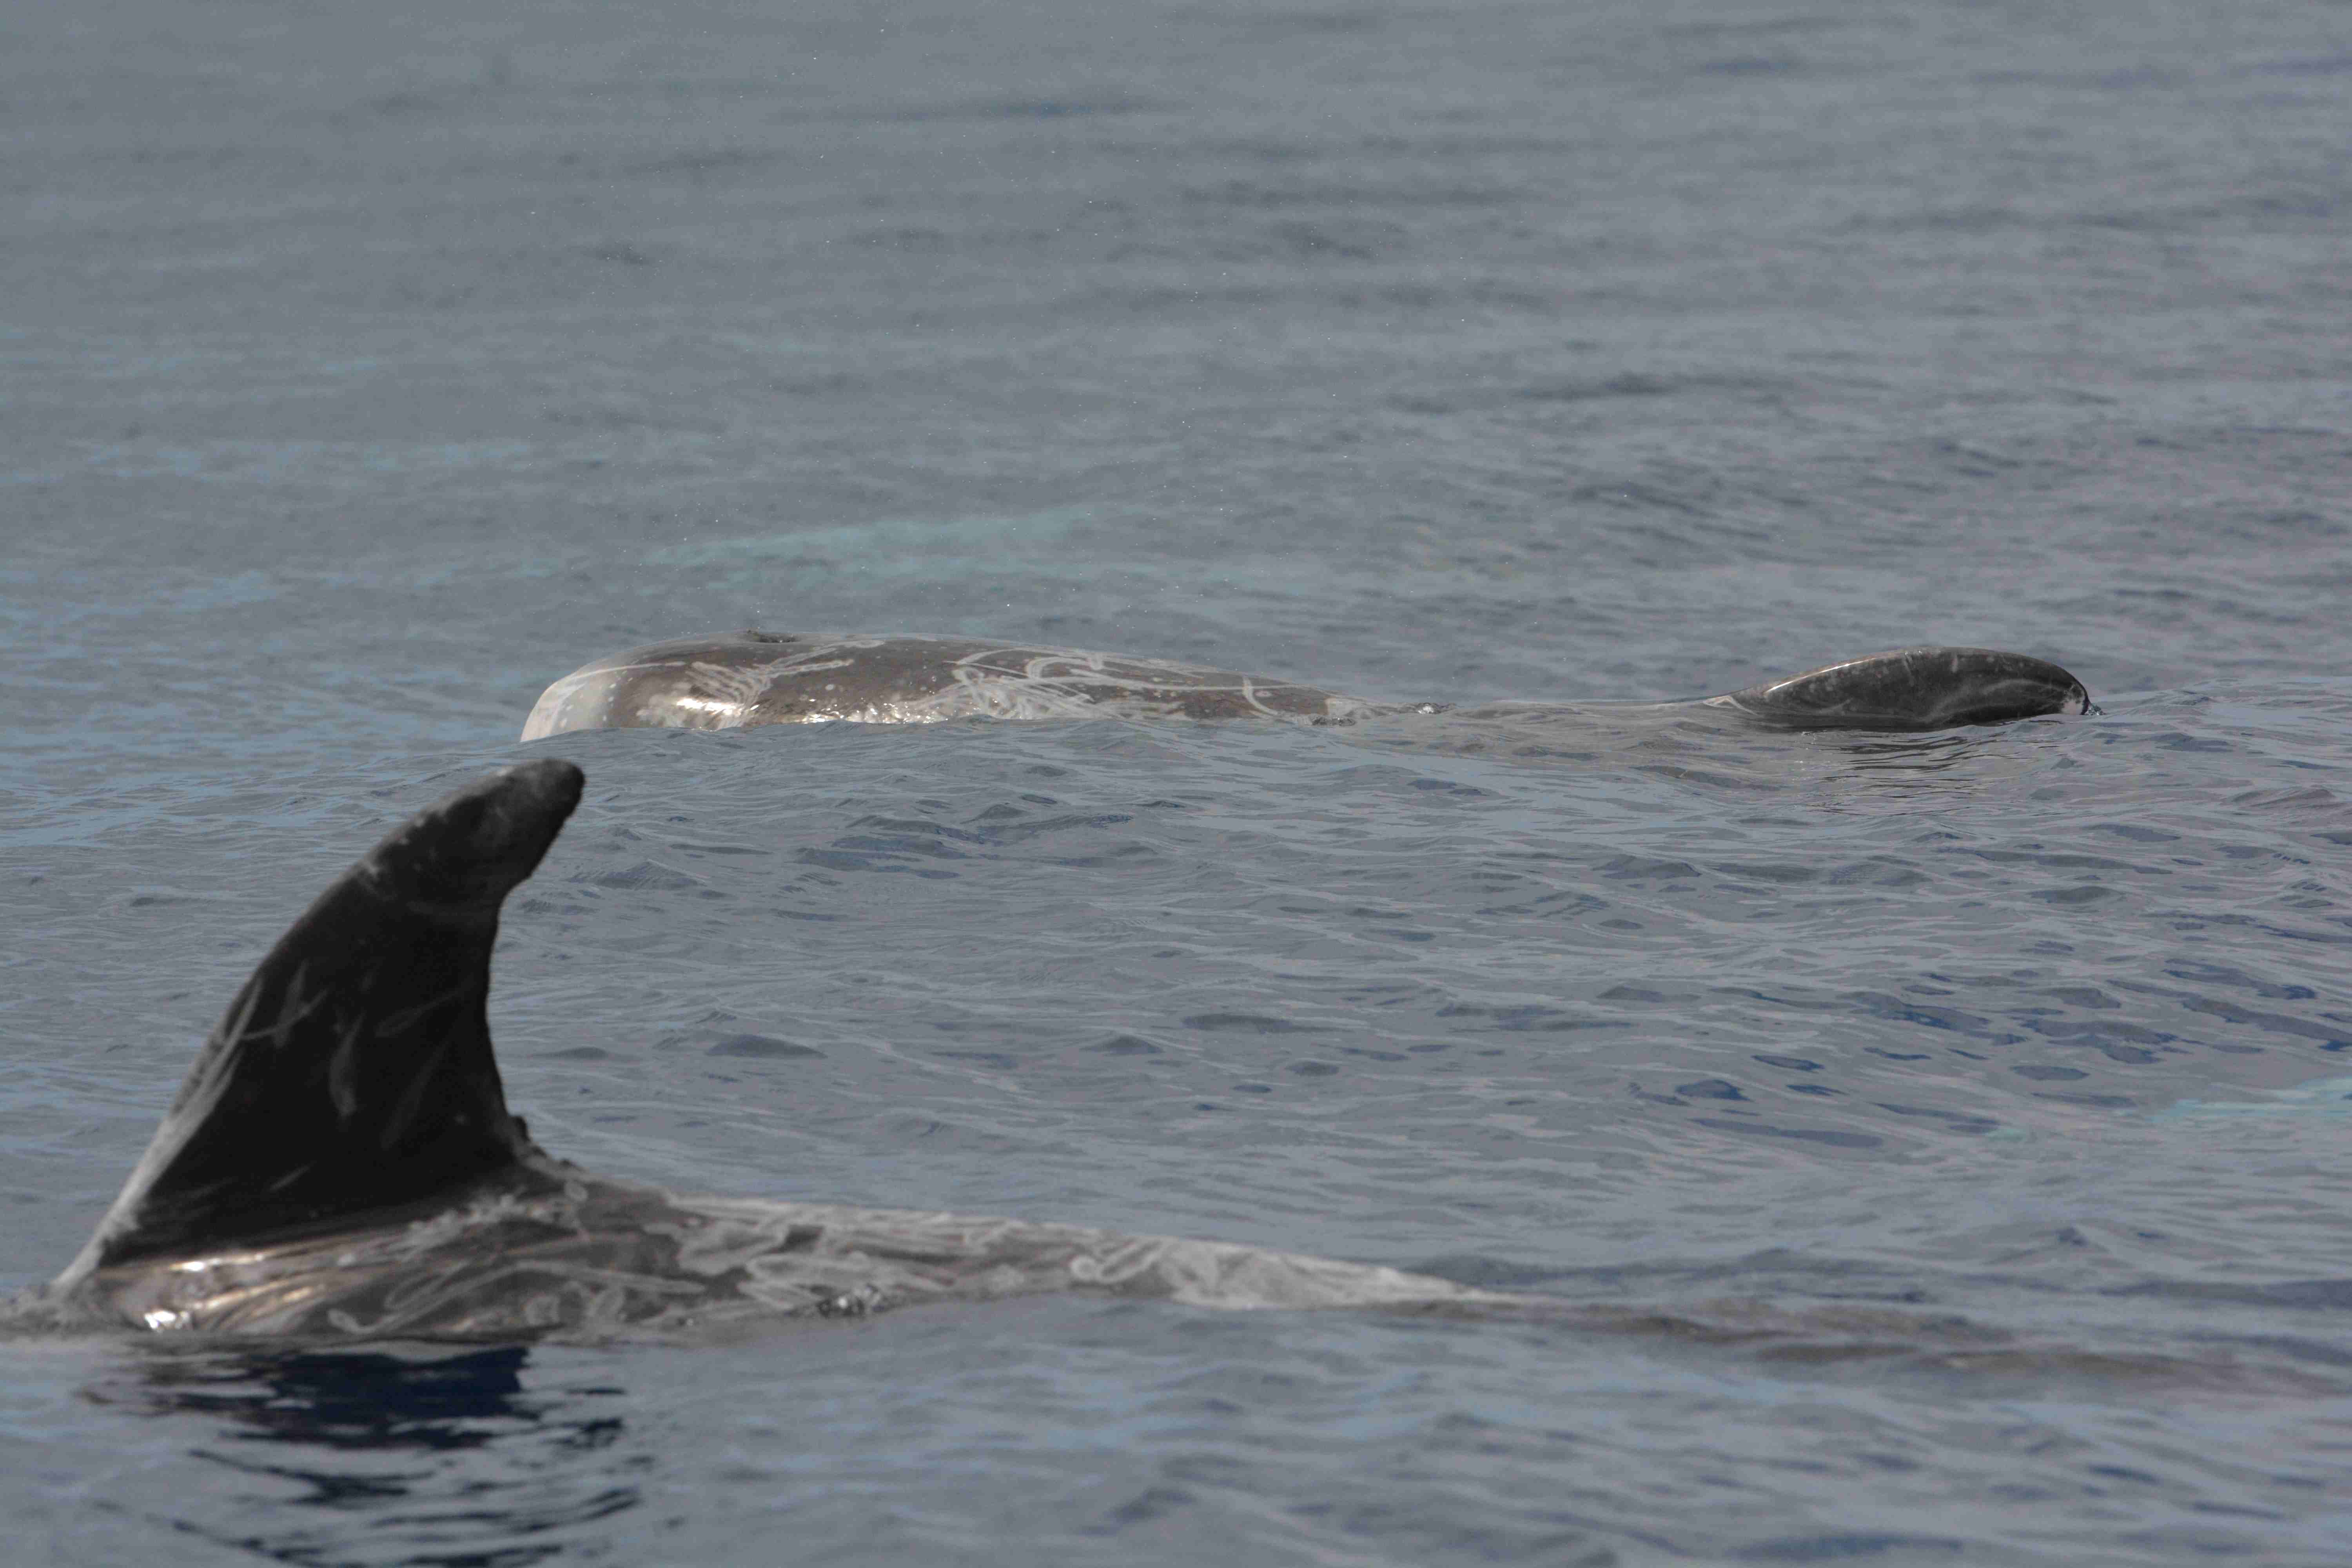
\includegraphics[width=0.24\linewidth]{a3.jpg}
    \hfill
    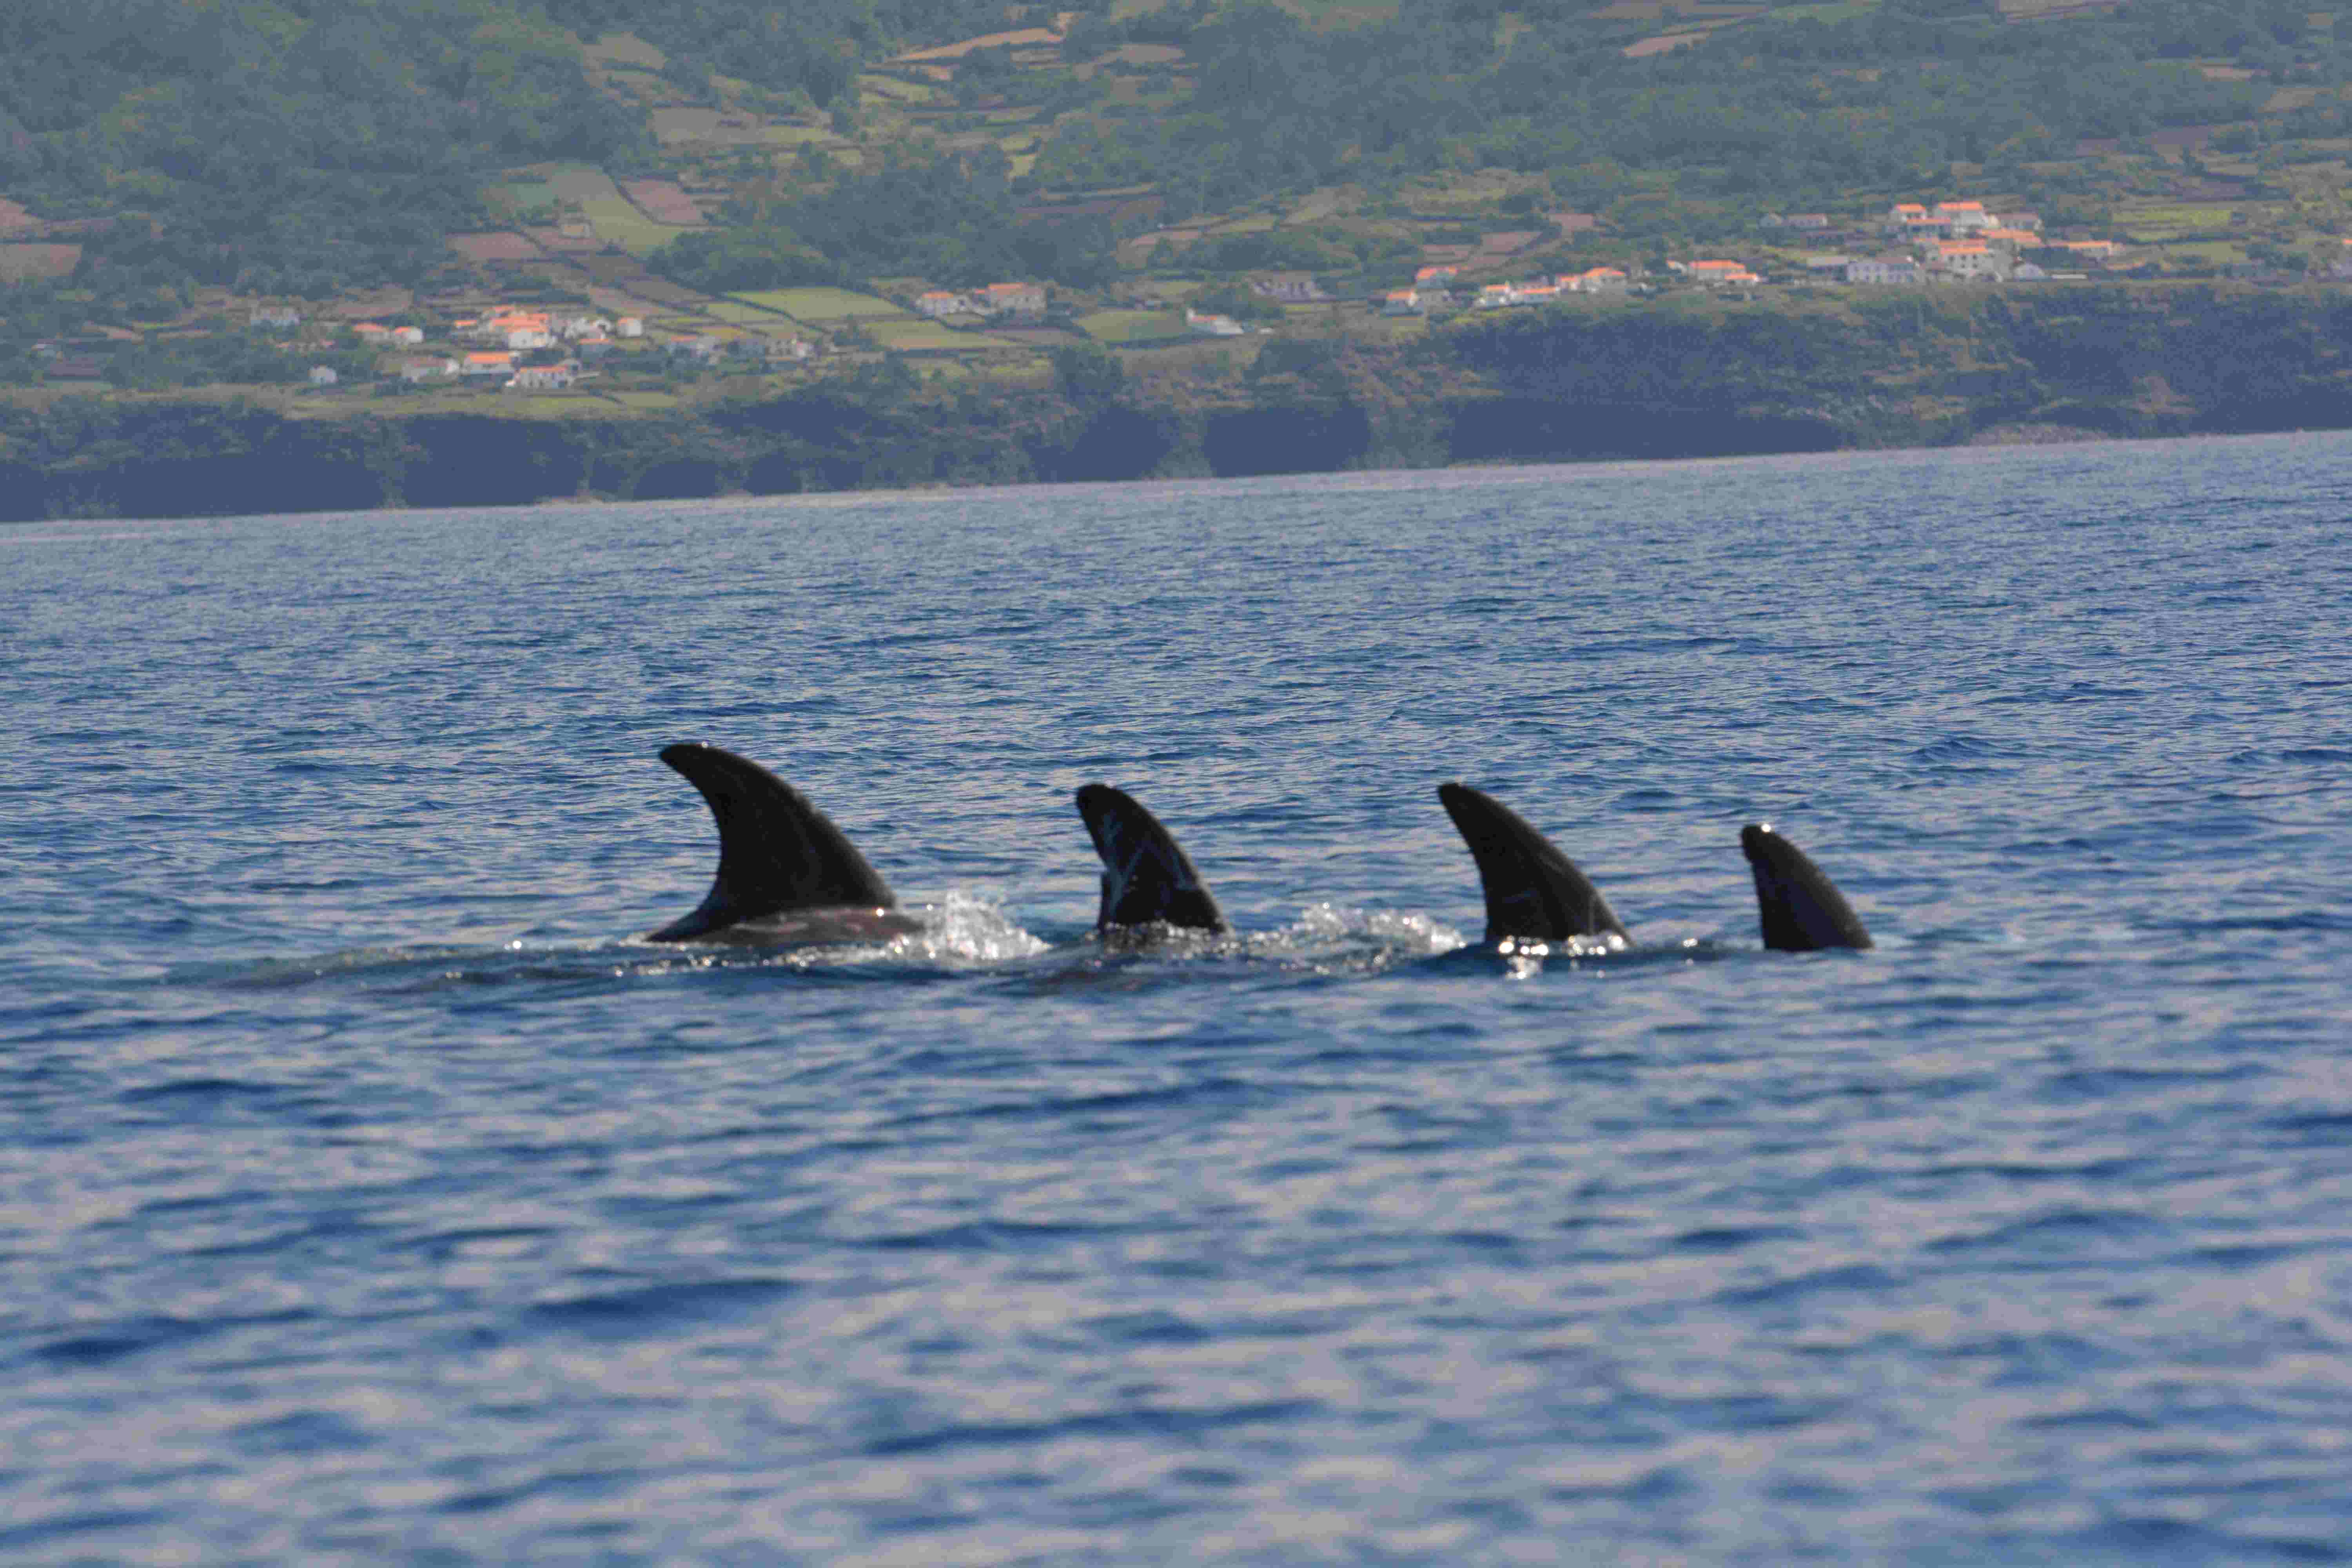
\includegraphics[width=0.24\linewidth]{a4.jpg}
    \caption{}
  \end{subfigure}
  
  \caption{Alcune immagini estrapolate dai due dataset utilizzati. (a) Dataset degli scatti di Taranto, (b) Dataset degli scatti delle Azzorre. Si noti la presenza di foto con disturbi o addirittura senza alcun valore informativo ai fini dello studio dei cetacei.}
  \label{fig:esempiDataset}
\end{figure}

Si rende perciò necessario filtrare in qualche modo le sole immagini che raffigurano al loro interno pinne dorsali di cetacei; è utile inoltre ritagliare da queste immagini filtrate le sole regioni in cui è effettivamente presente una pinna (si vuole cioè isolare l'informazione utile dal resto del dato originale). Per far questo, i due dataset sono stati rielaborati attraverso un \textbf{algoritmo di riconoscimento e cropping} delle pinne dorsali, di seguito descritto nelle sue caratteristiche salienti.

\section{CropFin v1}
\label{cropFin}
Per ritagliare ed estrarre dalle immagini originali le sole pinne dorsali, è stata utilizzata la routine \textit{CropFin v1} in linguaggio MATLAB sviluppata in \cite{gianvito} sulla base di un precedente lavoro  \cite{flavio}.
Si può descrivere la routine in due fasi:
\begin{enumerate}
\item Segmentazione, filtraggio e ritaglio adattivo delle regioni delle immagini che possono verosimilmente contenere una pinna
\item Classificazione di ogni ritaglio ottenuto in due classi 'Pinna' e 'No Pinna', mediante una rete neurale artificiale creata \textit{ad-hoc}.
\end{enumerate}

La novità introdotta dal presente lavoro di tesi in merito al problema di estrazione delle pinne da un'immagine riguarda l'utilizzo di un metodo di classificazione basato sul \textit{transfer learning}. In pratica, quindi, la principale differenza rispetto a CropFin v1 è nella seconda fase della routine: la classificazione avviene con l'utilizzo non più di una rete artificiale creata da zero per il problema in analisi, bensì riutilizzando un insieme di reti neurali profonde addestrate su un diverso problema di classificazione e adattate al nostro task. Questo nuovo modello è descritto dettagliatamente nel par. \ref{esperimentoTL}.\\

Al fine di ottenere i ritagli delle pinne, la routine adoperata attua una sequenza di operazioni di preprocessing su ciascuna immagine per poi individuare ed infine ritagliare e salvare separatamente le sole porzioni di immagini che possono eventualmente contenere pinne. Tale sequenza è implementata mediante un ciclo \verb|for| che cicla su ogni immagine del dataset. Di seguito sono descritte sinteticamente le operazioni, nell'ordine in cui vengono applicate. Le figure esplicative per ogni fase provengono dalla tesi triennale dell'ing. Losapio \cite{gianvito}, a cui vanno i crediti.

\subsection{Fase di ritaglio}
\label{faseRitaglio}

\subsection*{Ridimensionamento}
L'immagine è innanzitutto ridimensionata mediante la funzione MATLAB \verb|imresize| con un fattore di scale $\times 0.2$, al fine di ottenere una nuova immagine di risoluzione più bassa ($1200\times 800$).
Questa operazione di preprocessing è stata adottata per diminuire il costo computazionale delle operazioni successive.\footnote{La risoluzione di partenza delle immagini utilizzate è stata $6000\times 4000$, ottenendo una riduzione drastica di pixel del 96\%, da 24 milioni a 960 mila.}\\

\noindent Il risultato dell'operazione è visualizzato in figura \ref{fig:ridimensionamento}

\begin{figure}[h]
  \centering
  \begin{subfigure}[b]{0.475\textwidth}
    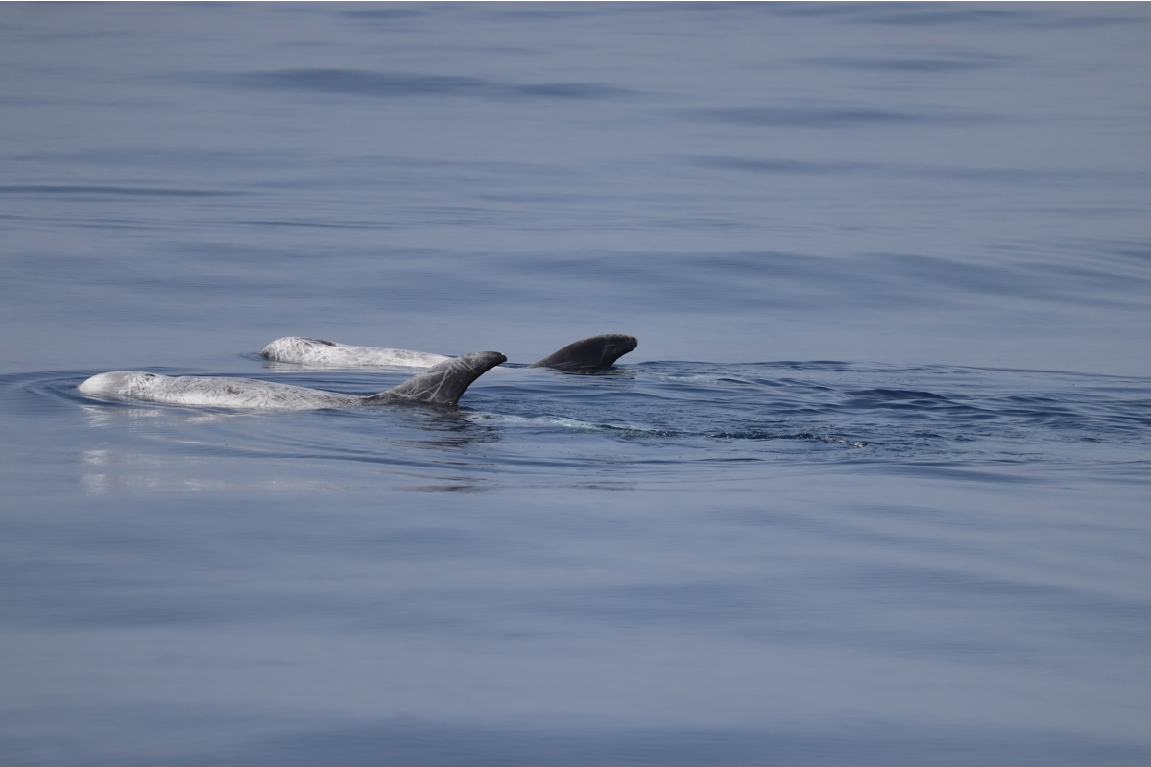
\includegraphics[width=\textwidth]{immagineDaProcessare.png}
    \caption{Prima del ridimensionamento}
  \end{subfigure}
  \begin{subfigure}[b]{0.475\textwidth}
  \centering
    \includegraphics[width=0.2\textwidth]{immagineDaProcessare.png}
    \caption{Dopo il ridimensionamento}
  \end{subfigure}
  \caption{Ridimensionamento di un'immagine (scelta nel dataset degli scatti di Taranto)}
  \label{fig:ridimensionamento}
\end{figure}


\subsection*{CLAHE}
L'immagine ridimensionata è sottoposta ad una equalizzazione adattiva dell’istogramma a contrasto limitato (CLAHE). Questa operazione consente un miglioramento del contrasto dell'immagine, proprietà utile per migliorare l'efficienza della successiva operazione, la sogliatura dell'immagine secondo il metodo di Otsu.\\

\noindent Il risultato dell'operazione è visualizzato in figura \ref{fig:clahe}

\begin{figure}[h]

  \centering
  
  \begin{subfigure}[b]{0.42\textwidth}
    \includegraphics[width=\textwidth]{primaClahe.jpg}
    \caption{Prima dell'applicazione di CLAHE}
  \end{subfigure}
  \begin{subfigure}[b]{0.42\textwidth}
  \centering
    \includegraphics[width=\textwidth]{dopoClahe.jpg}
    \caption{Dopo l'applicazione di CLAHE}
  \end{subfigure}
  
  \caption{Applicazione dell'equalizzazione CLAHE all'immagine, con visualizzazione dell'istogramma nello spazio dei colori \textit{L*a*b*}. NB: per semplicità l'immagine è raffigurata riportandola alle sue dimensioni originali}
  \label{fig:clahe}
\end{figure}

\subsection*{Segmentazione}
L'immagine viene segmentata (cioè ogni pixel viene assegnato ad una di due classi: \textit{background} e \textit{foreground}) mediante il metodo di Otsu per la sogliatura automatica \cite{otsu}.

Il metodo di Otsu viene usato nella sua versione classica a due livelli, rispetto agli istogrammi dei canali L e b. In particolare, viene applicata la sogliatura secondo Otsu separatamente al canale L e b, cioè calcolate le soglie di Otsu per i due canali, mediante la funzione \verb|multithresh|.
Avendo a disposizione tali soglie, l’ipotesi avanzata è che le pinne dorsali possano essere
isolate considerando le regioni di immagine che siano contemporaneamente:
\begin{itemize}
\item nella regione più scura del canale L, cioè a sinistra della soglia sul canale L
\item nella regione contenente il grigio del canale b, cioè a destra della soglia sul canale b
\end{itemize}
L'immagine segmentata (binarizzata) finale è ottenuta quindi annerendo quei pixel dell'immagine che non verificano le seguenti condizioni (o, equivalentemente, rendendo bianchi i pixel che le verificano)\footnote{L’idea alla base di questo approccio nasce da una precisa conoscenza del dominio e da alcune ipotesi a priori riguardanti il contenuto delle immagini. In particolare, si suppone
che esse contengano generalmente solo mare (background) e cetacei (foreground),
e che queste due classi di oggetti contribuiscano alla creazione di due aree distinte e
separabili degli istogrammi dei canali L e b. Volendo dare un’interpretazione intuitiva,
si tratta di separare ciò che è grigio e più scuro da ciò che è blu e più chiaro. La scelta
dello spazio di colori Lab è motivata proprio dalla possibilità di automatizzare questo
tipo intuitivo di segmentazione.}
\begin{itemize}
\item valore della componente L minore della soglia di Otsu sul canale L
\item valore della componente b maggiore della soglia di Otsu sul canale b
\end{itemize}

\noindent Il risultato dell'operazione è visualizzato in figura \ref{fig:otsu1}

\begin{figure}[h!]

  \centering
  
  \begin{subfigure}[b]{0.4\textwidth}
    \includegraphics[width=0.95\textwidth]{primaOtsu.jpg}
    \caption{Prima della segmentazione secondo Otsu}
  \end{subfigure}
  \begin{subfigure}[b]{0.4\textwidth}
    \includegraphics[width=0.95\textwidth]{dopoOtsu.jpg}
    \caption{Dopo la segmentazione secondo Otsu}
  \end{subfigure}
  
  \vspace{5mm}
  
  \begin{subfigure}[b]{0.5\textwidth}
  \centering
    \includegraphics[width=\textwidth]{otsu.jpg}
    \caption{Individuazione delle soglie di Otsu per i canali L e b sui relativi istogrammi}
  \end{subfigure}
  
  \caption{Applicazione della segmentazione secondo Otsu nello spazio dei colori \textit{L*a*b*}}
  \label{fig:otsu1}
\end{figure}

\subsection*{Filtraggio delle regioni connesse}
L’immagine binaria ottenuta in seguito alla segmentazione viene filtrata in modo che siano scartate quelle regioni binarie connesse (anche dette \textit{blob}) che non presentano caratteristiche tali da poter rappresentare, verosimilmente, una pinna dorsale.
In particolare vengono utilizzati, consecutivamente due filtri:
\begin{enumerate}

\item il primo è applicato all'intera immagine binarizzata e serve a migliorare il risultato della sogliatura secondo Otsu.
Il filtro è configurato per mantenere, nell'ordine, le regioni connesse con le seguenti proprietà:
\begin{itemize}
\item prime 15 in ordine decrescente di \verb|Area| (n. di pixel che compongono la regione connessa)
\item \verb|Area| nel range \verb|[1600, 40000]|
\item \verb|Extent| nel range \verb|[-Inf, 0.55]| (rapporto tra \verb|Area| e il n. di pixel del più piccolo rettangolo che racchiude l'intera regione connessa, con i lati paralleli a due a due paralleli ai bordi dell'immagine)
\end{itemize}

\item il secondo è applicato come segue
\begin{enumerate}
\item Si ritaglia la foto originale in corrispondenza delle regioni mantenute in seguito all’applicazione del primo filtro, sulla base delle coordinate dei bounding box. Per ottenere ritagli leggermenti più larghi rispetto ai blob, al fine di non perdere eventuali parti della pinna erroneamente anneriti dopo la binarizzazione, ogni dimensione è aumentata del 20\%.
\item Si applica nuovamente, a ciascun ritaglio ottenuto, la sogliatura basata sul metodo di Otsu. In questo caso è omesso il miglioramento del contrasto mediante CLAHE prima del calcolo dei valori di soglia.
\item Si introduce a questo punto il secondo filtro, applicato alle regioni binarie ottenute per ciascun ritaglio. L’unico parametro utilizzato in questo caso è il seguente:
\begin{itemize}
\item \verb|Area| nel range \verb|[20000, 1000000]|
\end{itemize}
con lo scopo di isolare l’eventuale pinna (che rappresenta sicuramente la regione di area maggiore all’interno di ciascun ritaglio) in modo che possa essere sottoposta all’algoritmo di ritaglio adattivo, descritto nella sezione successiva.
\end{enumerate}
\end{enumerate}

\noindent Il risultato dell'operazione è visualizzato in figura \ref{fig:filtraggioBlob}

\begin{figure}[h!]

  \centering
  
  \begin{subfigure}[b]{0.8\textwidth}
    \includegraphics[width=\textwidth]{dopoFiltroFoto.jpg}
  \caption{Prima dell'individuazione delle regioni connesse}
  \end{subfigure}
  
  \vspace{5mm}
  
  \begin{subfigure}[b]{0.3\textwidth}
    \includegraphics[width=0.95\textwidth]{ritaglioBlob.png}
  \caption{Estrazione
delle regioni connesse dall’immagine binarizzata}
  \end{subfigure}
  \begin{subfigure}[b]{0.3\textwidth}
    \includegraphics[width=0.95\textwidth]{dopoOtsuBlob.png}
  \caption{Applicazione ripetuta della sogliatura secondo Otsu (senza CLAHE)}
  \end{subfigure}
  \begin{subfigure}[b]{0.3\textwidth}
    \includegraphics[width=0.95\textwidth]{dopoFiltroBlob.png}
  \caption{Applicazione del secondo filtro sulle regioni connesse estratte}
  \end{subfigure}
  
  \caption{Fase di filtraggio delle regioni connesse}
  \label{fig:filtraggioBlob}
\end{figure}

\subsection*{Ritaglio adattivo}
Le regioni binarie mantenute in seguito alla fase di filtraggio sono sottoposte ad un algoritmo che consente di ottenere un ritaglio preciso in corrispondenza delle pinne.
Tale operazione si può definire "adattiva" nella misura in cui la regione di ritaglio è ottenuta a partire da precisi punti geometrici calcolati per ciascuna regione binaria.
Evitando di scendere nei dettagli implementativi e numerici (riportati nel par. 5.1 in \cite{gianvito}), si descrivono nell'ordine le operazioni effettuate sulle singole regioni binarie dall'algoritmo di ritaglio:
\begin{enumerate}
\item Si sottopone la regione binaria al riempimento dei cosiddetti \textit{holes}, cioè "buchi" anneriti racchiusi in una regione connessa, mediante la funzione \verb|imfill| con opzione \verb|'holes'|
\item Si individuano quattro punti di interesse; nell’ordine: punto più in alto, punto medio tra questo ed il centroide, punti di estrema sinistra e destra della regione connessa all’altezza del
punto medio
\item Si identifica il più piccolo rettangolo che racchiude i punti precedentemente trovati
\item Si trasla e si estende il rettangolo trovato in modo che contenga l’intera pinna, a seconda della sua orientazione.
\end{enumerate}

L'output di questa prima fase della routine sono i ritagli di quelle regioni dell'immagine originale che, verosimilmente, ritraggono una pinna dorsale. Questa ipotesi sul contenuto dei ritagli è sostenuta solamente sulla base del processo di segmentazione e filtraggio appena descritto.\\

\noindent Il risultato dell'operazione è visualizzato in figura \ref{fig:ritaglioAdattivo}\\

\begin{figure}[h!]

  \centering
  
  \begin{subfigure}[t]{0.475\textwidth}
    \includegraphics[width=0.95\textwidth]{ritaglio1.jpg}
    \caption{Regione binaria da sottoporre a ritaglio adattivo}
  \end{subfigure}
  \begin{subfigure}[t]{0.475\textwidth}
    \includegraphics[width=0.95\textwidth]{ritaglio2.jpg}
    \caption{Riempimento degli \textit{holes}}
  \end{subfigure}
  
  \vspace{5mm}
  
  \begin{subfigure}[b]{0.7\textwidth}
    \includegraphics[width=\textwidth]{ritaglio3.jpg}
    \caption{Individuazione dei quattro punti di interesse}
  \end{subfigure}
  
  \vspace{5mm}
  
  \begin{subfigure}[b]{0.7\textwidth}
    \includegraphics[width=\textwidth]{ritaglio4.jpg}
    \caption{Individuazione del rettangolo che racchiude i quattro punti di interesse}
  \end{subfigure}
  
  \vspace{5mm}
  
  \begin{subfigure}[b]{0.7\textwidth}
    \includegraphics[width=\textwidth]{ritaglio5.jpg}
    \caption{Traslazione ed estensione del rettangolo trovato}
  \end{subfigure}
  
  \vspace{5mm}
  
  \begin{subfigure}[b]{0.475\textwidth}
    \includegraphics[width=0.95\textwidth]{ritaglio6.jpg}
    \caption{Ritaglio di partenza}
  \end{subfigure}
  \begin{subfigure}[b]{0.475\textwidth}
    \includegraphics[width=0.95\textwidth]{ritaglio7.jpg}
    \caption{Risultato finale}
  \end{subfigure}
  
  \caption{Fase di ritaglio adattivo}
  \label{fig:ritaglioAdattivo}
\end{figure}

La routine CropFin v1, nella sua prima fase di ritaglio adattivo, è stata applicata ai dataset degli scatti di Taranto e delle Azzorre. In tabella \ref{risultatiCrop} è riportato il numero di ritagli (\textit{crops}) prodotti da CropFin v1 con input i dataset sopracitati.

\begin{table}[h]

  \centering
  \begin{tabular}{c c c c c}
  \hline
  Dataset&N. foto&N. crop&di cui 'Pinna'&di cui 'No Pinna'\\
  \hline
  Taranto&10194&15228&4033&11195\\
  Azzorre&11290&20395&3793&16602\\
  \hline
  \end{tabular}
  
  \caption{Output della prima fase di CropFin v1}
  \label{risultatiCrop}

\end{table}

\subsection{Fase di classificazione}
\label{faseClassificazione}

È evidente da una rapida ispezione dell'output che la quantità di regioni estratte che però non contengono pinne risulta, su larga scala, superiore a quella che contiene effettivamente pinne. Numericamente questo fatto è evidenziato in tab. \ref{risultatiCrop}, compilata dopo una fase di etichettatura a mano dei ritagli prodotti, nelle classi 'Pinna' e 'No Pinna' (motivata e spiegata nel seguito del sottoparagrafo). I ritagli della classe 'No Pinna' ottenuti sono l’esito "fallimentare" della procedura di segmentazione, filtraggio e ritaglio adattivo adottati in CropFin v1.

Questa osservazione è ciò che primariamente motiva l’introduzione di una fase di classificazione finale in CropFin v1, che consenta di automatizzare completamente la procedura di object detection.\\

La fase di classificazione prevede l'impiego di un classificatore binario che sappia discriminare un ritaglio in 'Pinna' o 'No Pinna'. L'addestramento di un tale classificatore (a prescindere dalle sue caratteristiche) può essere fatto mediante tecniche di supervised learning (par. \ref{supervisedLearning}), avendo a disposizione molti esempi "etichettati" di entrambe le classi da predire.

\subsection*{Creazione del training set}

Per consentire l'addestramento del classificatore si rende quindi necessario un lavoro di etichettatura manuale dei ritagli, attribuendo a ciascuno la classe 'Pinna' e 'No Pinna'. Questa operazione è stata svolta per entrambi i dataset a nostra disposizione; i risultati di questa etichettatura manuale sono presenti nella tab. \ref{risultatiCrop}.\\

Si precisa che, nella fase di etichettatura manuale, sono stati attribuiti alla classe 'Pinna' tutti e soli i ritagli contenenti una sola pinna in primo piano, intera o leggermente tagliata, escludendo invece quelli con pinne multiple e quelli con una presenza preponderante del dorso dei delfini. I ritagli con tali caratteristiche, infatti, sono considerati maggiormente affidabili ai fini di una successiva foto-identificazione automatica delle pinne (ad esempio con la routine "\textit{SPIR}" sviluppata e descritta in \cite{maglietta} e migliorata in \cite{emanuele}). Inoltre, questa scelta è stata anche motivata dall’intenzione di creare un "concetto univoco" utile a semplificare sia la selezione manuale sia l’apprendimento del classificatore.
In fig. \ref{fig:esempiPinnaNoPinna} sono riportati alcuni esempi di etichettatura dei ritagli.

\begin{figure}[h!]

  \centering
  
  \begin{subfigure}[b]{0.7\textwidth}
    \includegraphics[width=0.19\textwidth]{p1.jpg}
    \hfill
    \includegraphics[width=0.19\linewidth]{p2.jpg}
    \hfill
    \includegraphics[width=0.19\linewidth]{p3.jpg}
    \hfill
    \includegraphics[width=0.19\linewidth]{p4.jpg}
    \hfill
    \includegraphics[width=0.19\linewidth]{p5.jpg}
    \caption{}
  \end{subfigure}
  
  \vspace{5mm}
  
  \begin{subfigure}[b]{0.7\textwidth}
    \includegraphics[width=0.19\textwidth]{np1.jpg}
    \hfill
    \includegraphics[width=0.19\linewidth]{np2.jpg}
    \hfill
    \includegraphics[width=0.19\linewidth]{np3.jpg}
    \hfill
    \includegraphics[width=0.19\linewidth]{np4.jpg}
    \hfill
    \includegraphics[width=0.19\linewidth]{np5.jpg}
    \caption{}
  \end{subfigure}
  
  \caption{Alcuni ritagli etichettati manualmente come appartenenti alla classe (a) 'Pinna', (b) 'No Pinna'}
  \label{fig:esempiPinnaNoPinna}
\end{figure}

I due dataset così etichettati si prestano bene ad essere usati per addestrare un classificatore in grado di risolvere il task in esame.

\subsection*{Classificazione mediante rete \textit{ad-hoc}}
Tra i vari modelli di classificazione adottabili, in CropFin v1 si decide di progettare una rete neurale convoluzionale creata \textit{ad-hoc}, costruita cioè appositamente per risolvere il task in questione, da zero (\textit{from scratch}). L'addestramento del classificatore è avvenuto con i 15228 ritagli del dataset di Taranto.
Per i dettagli sull'architettura, l'addestramento e le prestazioni di questo classificatore \textit{ad-hoc} si rimanda al par. 4.4.2 di \cite{gianvito}.\\

In questo lavoro di tesi si è tentato un approccio diverso alla classificazione: si è provato a risolvere il task mediante il riutilizzo di CNN pre-addestrate, con la tecnica del \textit{Transfer Learning}.


\section{Classificazione mediante CNN e Transfer Learning}
\label{esperimentoTL}
Nel par. \ref{transferLearning} sono state esposte molteplici motivazioni per le quali per risolvere un problema di classificazione (in particolare di \textit{image classification}) può essere meglio usare la tecnica del \textit{transfer learning}, adattando al task in esame una rete neurale pre-addestrata piuttosto che creare una rete da zero.
Il nucleo principale di questo lavoro di tesi è quindi dedicato alla creazione di un nuovo modello di classificazione, basato su \textit{transfer learning}, che possa migliorare la fase di classificazione di CropFin v1. Questi "miglioramenti" sono da valutare con rigore ingegneristico sulla base di alcuni parametri, che consentono un confronto di prestazioni con il classificatore di CropFin v1; l'analisi delle prestazioni e quindi il confronto è svolto nel par. \ref{classEnsemble}.

\subsection{Scelta delle CNN}
Sono state riutilizzate ed adattate mediante la tecnica del \textit{transfer learning} quattro reti neurali convoluzionali (\textit{CNN}) sviluppate nell'ambito della \textit{ImageNet Large Scale Visual Recognition Challenge (ILSVRC)} ed addestrate sul dataset ImageNet (par. \ref{imagenet}). La loro scelta è stata motivata dal loro successo e prestigio nell'ambito del problema di \textit{object classification} proposto nella \textit{ILSVRC}. La scelta di queste reti è stata altresì motivata da un interesse puramente didattico, cioè studiare il funzionamento di CNN diverse per scelte architetturali e prestazioni, a prescindere dalla risoluzione del problema in esame. Esse sono di seguito elencate

\begin{itemize}

\item \textbf{AlexNet} (par. \ref{alexnet})\\
La sua vittoria nella \textit{ILSVRC 2012} con un tasso di errore \textit{top-5} del 16.4\% ha di fatto dimostrato alla comunità scientifica la straordinaria efficienza delle reti neurali convoluzionali nell'ambito dei problemi di \textit{computer vision}.

\item \textbf{GoogLeNet} (par. \ref{googlenet})\\
Grazie all'introduzione del modulo \textit{Inception}, GoogLeNet è una rete profonda ma incredibilmente leggera e semplice da addestrare, se paragonata alle precedenti reti fino ad allora esistenti (tra tutte, AlexNet).

\item \textbf{ResNet-18} (par. \ref{resnet})\\
ResNet rappresenta lo stato dell'arte nell'ambito delle reti neurali convoluzionali; l'introduzione dei \textit{residual blocks} ha permesso di avere reti con un grandissimo numero di layer, attenuando di molto i problemi legati all'estrema profondità dell'architettura.

\item \textbf{ResNet-50} (par. \ref{resnet})\\
Una variante di ResNet, più profonda e con migliori prestazioni sul dataset \textit{ImageNet}.

\end{itemize}

\subsection{Addestramento}
\label{addestramento}
L'ambiente di sviluppo nel quale sono state addestrate le quattro reti è il software Matlab R2019a, esteso con il pacchetto \textit{Deep Learning Toolbox}. Tutto il codice sorgente Matlab creato è riportato nel cap. \ref{sorgenti}.\\

Il dataset utilizzato per l'addestramento è quello con gli $n=15228$ ritagli che CropFin ha prodotto dagli scatti di Taranto (vd. tab. \ref{risultatiCrop}) e in seguito opportunamente etichettati a mano (come descritto nel par. \ref{faseClassificazione}). Questo dataset è di fatto lo stesso usato per l'addestramento del classificatore \textit{ad-hoc} in \cite{gianvito}.

Il dataset dei ritagli è rappresentato in Matlab da un oggetto \verb|imageDatastore|, ed è stato suddiviso (\textit{splitted}) in maniera casuale in due ulteriori oggetti \textit{imageDatastore}:

\begin{itemize}
\item \begin{frame}\space \verb|cropTrain|\end{frame}, un \textit{training set} contenente il 70\% dei ritagli (10659 ritagli), cioè il 70\% dei ritagli 'No Pinna' (7836) più il 70\% dei ritagli 'Pinna' (2823)
\item \begin{frame}\space \verb|cropValidation|\end{frame}, un \textit{validation set} contenente il rimanente 30\% dei ritagli (4569 ritagli di cui 3359 'No Pinna' e 1210 'Pinna')
\end{itemize}

Il training set è sottoposto ad operazioni di \textit{image augmentation} durante la fase di addestramento, per migliorare la capacità di generalizzazione del classificatore da addestrare ed evitare quindi l'\textit{overfitting}.
A ciascuna immagine del set sono applicate le seguenti trasformazioni, rappresentate in un opportuno oggetto \verb|imageDataAugmenter|:

\begin{itemize}
\item una riflessione rispetto all’asse x (operata con il 50\% di probabilità);
\item una rotazione di un angolo casualmente estratto dall’intervallo $[-20, 20]$ gradi;
\item una traslazione sull’asse x di una quantità casualmente estratta dall’intervallo
$[-60, 60]$ pixel.
\end{itemize}

\noindent Un oggetto \verb|augmentedImageDatastore| parametrizzato con l'\verb|imageDataAugmenter| sopra descritto e l'\verb|inputSize| della rete è creato per rappresentare la versione "aumentata" di \verb|cropTrain|.
Le operazioni applicate in maniera casuale contribuiscono ad ottenere ulteriore variabilità del dataset impiegato per la fase di addestramento; i ritagli vengono inoltre ridimensionati all'input size della rete da addestrare. Si è ritenuto opportuno impiegare poche trasformazioni ad effetto limitato: le uniche che non alterassero eccessivamente il contenuto dei ritagli di classe Pinna rispetto al problema in esame ed al dataset a disposizione (già di per sè contenente grande variabilità relativa alla classe Pinna).

\begin{figure}[h!]
  \centering
  \includegraphics[width=0.75\textwidth]{augmentation.png}
  \caption{Un campione di ritagli sottoposti alle operazioni di \textit{augmentation}}
  \label{fig:augmentation}
\end{figure}

Un secondo oggetto \verb|augmentedImageDatastore| è usato per rappresentare la versione "aumentata" di \verb|cropValidation|, ma in questo caso è parametrizzato solo con \verb|inputSize| (viene cioè effettuato solamente un ridimensionamento dei ritagli all'input size della rete da addestrare, senza operazioni di augmentation).

Si noti che i due dataset "aumentati" hanno le stesse dimensioni dei loro omologhi dataset "non aumentati", nel senso che ogni ritaglio del dataset originale è presente esattamente una volta nel relativo dataset aumentato: l'unica differenza tra il ritaglio originale e quello nel dataset aumentato è appunto l'applicazione (a \textit{runtime}) delle operazioni di ridimensionamento e -- nel caso del \textit{training set} -- augmentation a ciascun ritaglio. Si tratta quindi di una semplice "perturbazione" dei due dataset, senza eliminazione di suoi elementi o aggiunta di nuovi.\\

L'inizializzazione delle quattro CNN all'interno dell'ambiente Matlab è particolarmente semplice, e può essere effettuato richiamando la rete col suo nome (\verb|alexnet|, \verb|googlenet|, \verb|resnet18|, \verb|resnet50|) assegnandola ad una variabile, avendo cura di scaricare il relativo \textit{add-on} dall'\textit{add-on explorer} integrato di Matlab, estendendo il \textit{Deep Learning Toolbox}.

Le quattro reti, come visto nei rispettivi paragrafi, sono in origine state addestrate sul database di immagini \textit{ImageNet} (par. \ref{imagenet}) per classificare un'immagine scegliendo tra le mille categorie diverse del dataset. Applicare la tecnica del \textit{transfer learning} (par. \ref{transferLearning}) per adattare ciascuna rete al problema di classificazione binaria delle pinne significa effettuare le seguenti operazioni

\begin{itemize}
\item analizzare l'architettura della rete e decidere quanti e quali layer (tra quelli dotati di parametri addestrabili) "congelare", cioè impedirne l'ulteriore \textit{fine-tuning} dei  parametri in fase di ri-addestramento azzerando il learning rate dei layer
\item sostituire nella rete originale da "trasferire" l'ultimo \textit{fully-connected layer} avente 1000 neuroni, ognuno associato alle 1000 classi del database ImageNet e il cui valore di attivazione permette di calcolare la probabilità per la relativa classe (attraverso la funzione \textit{softmax}), con un nuovo \textit{fully-connected layer} dotato di 2 soli neuroni, relativi alle classi 'Pinna' e 'No Pinna'; questo nuovo layer è inizializzato con un learning rate abbastanza alto (fissato a 10) per permettere un addestramento più veloce
\item adattare la nuova rete così creata al problema di classificazione binaria delle pinne grazie al ri-addestramento della rete sul nuovo dataset dei ritagli, descritto in precedenza
\end{itemize}

Si noti che per la scelta di quanti e quali layer parametrizzati "congelare" non esistono regole o criteri generali; questa scelta è un nuovo set di iperparametri della rete, da trovare risolvendo uno specifico problema di ottimizzazione degli iperparametri. Poiché per ottimizzare questi iperparametri sarebbe necessario addestrare un gran numero di volte ciascuna delle quattro reti, con un notevole impiego di tempo, tale problema di ottimizzazione non è stato risolto in questa sede e si è preferito scegliere manualmente i layer da congelare.

Per garantire un buon \textit{trade-off} tra capacità di generalizzazione sul nuovo dataset e velocità di addestramento della rete, si è scelto di congelare uno, due o tre layer convoluzionali iniziali di ciascuna rete, nell'ordine in cui sono presenti nell'architettura della rete.
Tale scelta è motivata anche dal fatto che il dataset \textit{ImageNet} e quello dei ritagli delle pinne hanno alcune caratteristiche in comune: nel primo ci sono almeno una decina di classi diverse di cetacei, come ad esempio 'gray whale' (balena grigia) e 'killer whale' (orca).
Mutuando un'idea discussa in \cite{howtransferable}, si è quindi avanzata la plausibile ipotesi che tutte le reti abbiano imparato, nei livelli più bassi, ad estrarre \textit{features} abbastanza generali utili per il riconoscimento di una variegata classe di animali marini e delle loro parti del corpo, e pertanto questi primi layer possono essere riutilizzati senza modifiche.
Per ulteriori dettagli sull'implementazione in Matlab riferirsi al cap. \ref{sorgenti}.\\

Per ogni classificatore, l’addestramento è stato eseguito con il metodo \textit{stochastic gradient descent with momentum}, con dimensione del \textit{minibatch} pari a 20, numero di epoche pari a 6 e \textit{learning rate} globale pari a 0.0003.
Ciò ha portato alla definizione del seguente oggetto \verb|trainingOptions|:

\begin{verbatim}
miniBatchSize = 20;
valFrequency = floor(numel(cropAugmentedTrain.Files)/miniBatchSize);

options = trainingOptions('sgdm', ...
    'MiniBatchSize',miniBatchSize, ...
    'MaxEpochs',6, ...
    'InitialLearnRate',3e-4, ...
    'Shuffle','every-epoch', ...
    'ValidationData', cropAugmentedValidation, ...
    'ValidationFrequency',valFrequency, ...
    'Verbose',true, ...
    'Plots','training-progress', ...
    'CheckpointPath','.\Checkpoint [nome della rete]');
\end{verbatim}

Il numero di epoche di addestramento, relativamente basso, è accettabile in quanto utilizzando il transfer learning per ri-addestrare una rete pre-addestrata tipicamente sono necessarie poche iterazioni sull'intero dataset per ottenere un buon adattamento della rete al nuovo task di classificazione\footnote{come evidenziato in \url{https://it.mathworks.com/help/deeplearning/examples/transfer-learning-using-alexnet.html}}; inoltre un numero basso di epoche, assieme alle operazioni di augmentation, garantisce una discreta robustezza contro l'\textit{overfitting}, problema in cui si può facilmente incappare in presenza di un dataset di dimensioni relativamente ridotte come in questo caso.

Per quanto riguarda gli altri iperparametri (\textit{learning rate} globale e dimensione del \textit{minibatch}), i loro valori sono stati scelti empiricamente, sulla base di alcune \textit{best practices} generali presenti in letteratura\textsuperscript{3}, che funzionano bene con un'ampia classe di reti neurali convoluzionali e di dataset.
A rigore, i valori migliori per questi iperparametri possono essere trovati con la risoluzione di un preciso problema di ottimizzazione (che richiederebbe numerosi ri-addestramenti per ogni rete, con notevole dispendio di tempo). Tuttavia, come sarà evidente al momento della presentazione dei risultati, le prestazioni registrate dalle reti con questi iperparametri sono eccellenti, e non è necessario cercarne di migliori (un tale sforzo computazionale e di tempo non giustificherebbe un leggerissimo aumento dell'accuratezza).\\

\noindent L’addestramento di ciascuna rete è stato lanciato mediante la funzione
\begin{verbatim}
TL_net = trainNetwork(cropAugmentedTrain,layers,options)
\end{verbatim}
specificando il \textit{training set} sottoposto ad \textit{augmentation}, l’architettura della rete (array di tipo \verb|Layer| nel caso di AlexNet e di tipo \verb|LayerGraph| per le restanti reti) e le opzioni per l'addestramento.\\

\noindent Nella tabella \ref{prestazioniReti} sono riassunte le principali informazioni e i risultati globali (accuratezza sul \textit{validation set} e dati della matrice di confusione) di ciascuna rete così addestrata. Nelle figure dalla \ref{graficoAlexnet} alla \ref{graficoResnet50} sono riportati i grafici che mostrano l'andamento temporale dei quattro addestramenti.
L'addestramento è avvenuto nella modalità a singolo processore grafico su due diverse macchine:

\begin{itemize}

\item l'addestramento di AlexNet, GoogLeNet e ResNet-18 è avvenuto su una macchina equipaggiata con CPU Intel Core i5-4670 @ 3.40 GHz con 8 GB di RAM e Intel HD Graphics 4600 (scheda video integrata)

\item l'addestramento di ResNet-50, decisamente più costoso a livello computazionale per via dei suoi numerosi pesi, è avvenuto su una workstation HP Z840 equipaggiata con due CPU Intel Xeon E5-2699 v3 @ 2.30 GHz, 256 GB di RAM e scheda video NVIDIA Quadro K5200 con 8 GB dedicati.

\end{itemize}

\begin{table}[h]

  \centering
  \begin{adjustbox}{width=1\textwidth}
  %\small
  \begin{tabular}{c c c c c c c c c}
  \hline
  Rete&Tempo addestramento&Accuracy&Sensitivity&Specificity&TP&FP&TN&FN\\
  \hline
  AlexNet&67m54s&99.87\%&99.75\%&99.91\%&1207&3&3356&3\\
  GoogLeNet&149m59s&99.89\%&99.67\%&99.97\%&1206&1&3358&4\\
  ResNet-18&168m17s&99.89\%&99.75\%&99.94\%&1207&2&3357&3\\
  ResNet-50&497m33s&90.30\%&98.93\%&87.20\%&1197&430&2929&13\\
  \hline
  \end{tabular}
  \end{adjustbox}
  
  \caption{Risultati del ri-addestramento delle quattro reti secondo la tecnica del \textit{transfer learning}}
  \label{prestazioniReti}

\end{table}

\begin{figure}[h!]
  \centering
  \includegraphics[width=0.88\textwidth]{TrainingAlexNet.png}
  
  \caption{Grafico del ri-addestramento di AlexNet}
  \label{graficoAlexnet}

\end{figure}

\begin{figure}[h!]
  \centering
  \includegraphics[width=0.88\textwidth]{TrainingGoogLeNet.png}
  
  \caption{Grafico del ri-addestramento di GoogLeNet}
  \label{graficoGooglenet}

\end{figure}

\begin{figure}[h!]
  \centering
  \includegraphics[width=0.88\textwidth]{TrainingResNet18.png}
  
  \caption{Grafico del ri-addestramento di ResNet-18}
  \label{graficoResnet18}

\end{figure}

\begin{figure}[h!]
  \centering
  \includegraphics[width=0.88\textwidth]{TrainingResNet50.png}
  
  \caption{Grafico del ri-addestramento di ResNet-50.  Si noti che la \textit{training accuracy} è prossima al 100\% mentre la \textit{validation accuracy} si attesta al 90\%, chiaro sintomo di \textit{overfitting} al training set}
  \label{graficoResnet50}

\end{figure}

Con la sola esclusione di ResNet-50, i valori di accuratezza ottenuti, calcolati sul \textit{validation set}, sono molto elevati. Il successo ottenuto da questi classificatori nel risolvere il problema di classificazione delle pinne è dovuto probabilmente alla facilità con cui la rete riesce ad adattarsi al nuovo dominio di applicazione (d'altronde, è una classificazione binaria abbastanza semplice, a maggior ragione per reti molto profonde in grado di risolvere problemi di classificazione ben più complessi). Diverso è il caso di ResNet-50: per quanto comunque alta, l'accuratezza raggiunta del 90.30\% non è paragonabile a quella delle rimanenti tre reti. Si avanza quindi l'ipotesi di \textit{overfitting} della rete al \textit{training set}. Questa ipotesi è corroborata dal fatto che l'accuratezza valutata sul \textit{training set} è invece prossima al 100\%, come si nota in fig. \ref{graficoResnet50}. Questa mancata capacità di generalizzazione può essere conseguenza dell'eccessiva complessità della rete (n. di parametri inutilmente elevato), in rapporto ad un \textit{training set} relativamente piccolo\footnote{Delle considerazioni simili sono state fatte anche nel paper originale di ResNet \cite{resnet}.}.\\

Le performance delle quattro reti sono state, inoltre, misurate sul dataset dei ritagli ottenuti con CropFin v1 dal dataset degli scatti nelle Azzorre, di dimensione $n=20395$ (usato quindi come \textit{test set}). Si ricorda che questi ritagli erano stati in precedenza etichettati manualmente, come descritto nel par. \ref{faseClassificazione}. I risultati sono riassunti in tabella \ref{prestazioniRetiAzzorre}.

\begin{table}[h]

  \centering
  \begin{adjustbox}{width=1\textwidth}
  %\small
  \begin{tabular}{c c c c c c c c c}
  \hline
  Rete&Accuracy&Sensitivity&Specificity&TP&FP&TN&FN\\
  \hline
  AlexNet&97.1\%&97.9\%&96.9\%&3712&511&16091&81\\
  GoogLeNet&97.2\%&98.0\%&97.0\%&3718&493&16109&75\\
  ResNet-18&96.7\%&99.0\%&96.3\%&3754&619&15983&39\\
  ResNet-50&77.9\%&98.1\%&73.3\%&3722&4431&12171&71\\
  \hline
  \end{tabular}
  \end{adjustbox}
  
  \caption{Prestazioni valutate sul dataset dei ritagli delle Azzorre, usato come \textit{test set}}
  \label{prestazioniRetiAzzorre}

\end{table}

Come ci si aspettava, le reti hanno prestazioni abbastanza elevate, ad eccezione di ResNet-50. L'inefficienza di quest'ultima rete è aggravata dal fatto che la sua specificity sia risultata bassa: confondere un ritaglio 'No Pinna' con un ritaglio 'Pinna' è, dal punto di vista dell'utente (tipicamente un ricercatore), più grave del contrario. Infatti, è tollerabile perdere qualche pinna nei falsi negativi (in una spedizione uno stesso esemplare è spesso immortalato in più fotografie, quindi c'è un'alta probabilità che le sue pinne siano presenti in più ritagli di cui almeno uno correttamente classificato come 'Pinna'), ma è meno tollerabile avere molti falsi positivi (infatti gli algoritmi di foto-identificazione delle pinne come quello proposto in \cite{emanuele} danno sempre in output un \textit{match} plausibile, anche se l'input non raffigura una pinna).

Per questo motivo, d'ora in avanti ResNet-50 non verrà più utilizzata.

\subsection{Classificatore ensemble}
\label{classEnsemble}
Al fine di migliorare ulteriormente l'accuratezza della classificazione, si è sperimentato un metodo di apprendimento ensemble (\textit{ensemble learning}, par. \ref{ensemble}). L'idea chiave è quella di creare un insieme (\textit{ensemble}) di classificatori, ciascuno dei quali è chiamato a "votare" circa l'esito della predizione; a seconda dello "schema di consenso" (\textit{consensus scheme}) scelto per l'ensemble, cioè a seconda di quanto peso assume ciascun voto nella classificazione finale, l'output complessivo sarà la classe che avrà ricevuto "democraticamente" il maggior consenso.

Come già descritto nel par. \ref{ensemble}, l'efficacia dei metodi ensemble è dovuta al fatto che, solitamente, differenti modelli  addestrati per risolvere uno stesso problema di classificazione non faranno tutti gli stessi errori sul \textit{test set} (gli errori si possono cioè considerare, in buona sostanza, incorrelati). Se lo schema di consenso applicato è il \textit{major voting}, si dimostra che l'ensemble di classificatori ha sempre prestazioni migliori o almeno uguali a quelle di ciascuna rete dell'ensemble presa singolarmente; il miglioramento delle prestazioni è tanto migliore quanto più gli errori commessi dalle reti dell'ensemble sono tra loro incorrelati.\cite{dlbook}\cite{ensembles}\\

\noindent L'ensemble utilizzato è costituito dalle reti AlexNet, GoogLeNet e ResNet-18, addestrate sul dataset dei ritagli di Taranto. Uno schema dell'ensemble è raffigurato in fig. \ref{fig:ensemble}

\begin{figure}[h]
\centering
\includegraphics[width=0.8\textwidth]{ensemble.png}
\caption{Schema del classificatore ensemble creato}
\label{fig:ensemble}
\end{figure}

Sono stati effettuati due esperimenti che adottano due diversi schemi di consenso, di seguito elencati:

\begin{itemize}

\item \textbf{\textit{soft major voting}}: un ritaglio è classificato come 'Pinna' se la media delle probabilità attribuite alla classe 'Pinna' da ciascuna rete è maggiore del 50\%. La nuova probabilità attribuita alla classe 'Pinna' è appunto la suddetta media. Vale allo stesso modo il viceversa relativamente alla classe 'No Pinna'.

\item \textbf{\textit{hard major voting} con soglia}: un ritaglio è classificato come 'Pinna' se almeno due delle tre reti lo classificano come 'Pinna' e se inoltre la media delle probabilità attribuite alla classe 'Pinna' da ciascuna rete è maggiore di una certa soglia, fissata arbitrariamente al 97\%. La nuova probabilità attribuita alla classe 'Pinna' è appunto la suddetta media. Vale allo stesso modo il viceversa relativamente alla classe 'No Pinna'.

\end{itemize}

Gli esperimenti consistono nella classificazione del \textit{test set} contenente i ritagli delle Azzorre da parte del classificatore ensemble. Questi esperimenti hanno come scopo la misurazione delle prestazioni del classificatore ensemble, e consentono il confronto di prestazioni tra questo nuovo modello e quello di CropFin v1, descritto in \cite{gianvito} (e provato sullo stesso \textit{test set}). I risultati dei due esperimenti sono riportati in tabella \ref{prestazioniEnsemble}, assieme a quello relativo al classificatore nativo in CropFin v1.
Gli stessi dati riportati nella tabella \ref{prestazioniEnsemble} sono mostrati sotto forma di matrici di confusione in fig. \ref{fig:confMatEnsemble}.
In figura \ref{testHMVT} si riportano infine alcuni campioni di ritagli classificati dall'ensemble.\\


\begin{table}[h]

  \centering
  \begin{adjustbox}{width=1\textwidth}
  %\small
  \begin{tabular}{c c c c c c c c c}
  \hline
  Modello&Accuracy&Sensitivity&Specificity&TP&FP&TN&FN\\
  \hline
  Ensemble (SMV)&97.2\%&98.7\%&96.9\%&3745&518&16084&48\\
  Ensemble (HMVT)&97.2\%&93.4\%&98.1\%&3543&313&16289&250\\
  CropFin v1&92\%&85\%&95\%&--&--&--&--\\
  \hline
  \end{tabular}
  \end{adjustbox}
  
  \caption{Prestazioni di differenti modelli di classificazione, valutate sul dataset dei ritagli delle Azzorre. Abbreviazioni: SMV = \textit{soft major voting}, HMVT = \textit{hard major voting} con soglia (\textit{threshold}) sulla probabilità media}
  \label{prestazioniEnsemble}
  %\vspace{10mm}

\end{table}



\begin{figure}[h!]

  \centering
  
  \begin{subfigure}[b]{0.45\textwidth}
  \raggedright
    \includegraphics[width=\textwidth]{confMatAzzorreSMV.png}
    \caption{}
  \end{subfigure}
  \begin{subfigure}[b]{0.45\textwidth}
  \raggedleft
    \includegraphics[width=\textwidth]{confMatAzzorreHMVT.png}
    \caption{}
  \end{subfigure}
  
  \caption{Matrici di confusione relative alle predizioni del nuovo ensemble sui ritagli delle Azzorre, con schema di consenso (a) \textit{soft major voting}, (b) \textit{hard major voting} con soglia.}
  \label{fig:confMatEnsemble}
\end{figure}


\begin{figure}[h]
\centering
\includegraphics[width=\textwidth]{testHMVT.png}
\caption{Alcune predizioni proposte dall'ensemble con schema di consenso HMVT. Si noti ad esempio quella centrale in alto: compaiono tre pinne di cui addirittura due sovrapposte, ma il classificatore restituisce 'Pinna'. Sebbene il classificatore sia riuscito a confermare la presenza di una pinna, l'etichetta corretta era 'No Pinna' (per i criteri di etichettatura adottati sui ritagli con pinne multiple). Evidentemente nel training set con i ritagli di Taranto non erano presenti molti ritagli con pinne multiple, quindi il classificatore ha avuto difficoltà ad attribuire la classe 'No Pinna' a questo tipo di ritagli.}
\label{testHMVT}
\end{figure}


Confrontando le prestazioni ottenute dal classificatore di CropFin v1 e i due classificatori ensemble creati sfruttando il principio del \textit{transfer learning} è evidente la maggiore efficienza di questi ultimi, in tutti i parametri messi a confronto.

Si fa notare infine che lo schema di consenso di tipo HMVT ha fatto registrare un miglioramento del parametro di \textit{specificity} che, come spiegato in precedenza, è un parametro fondamentale in quanto dà una misura di quanto i ritagli classificati come 'Pinna' sono "sporcati" da ritagli 'No Pinna' erroneamente classificati come 'Pinna', un errore che l'utente finale vorrebbe evitare. Si può verificare che alzando la soglia sopra il 97\% la \textit{specificity} aumenta ancora, ma a scapito della \textit{sensitivity}, che decresce con una velocità purtroppo maggiore della \textit{specificity}. Tuttavia questo non costituisce un grosso problema nel caso in cui, come spesso avviene, ci sia una discreta ridondanza nella presenza di uno stesso esemplare in più foto di una stessa spedizione in mare, come descritto in precedenza\footnote{In questo caso, infatti, è meno probabile che in un dataset di ritagli da scatti avvenuti in una specifica spedizione vengano scartati \emph{tutti} i ritagli relativi alla pinna di un certo esemplare}.

In conclusione, quindi, si può affermare che adattare al nostro task di classificazione di ritagli di pinne un'opportuna rete neurale convoluzionale pre-addestrata con il metodo del \textit{transfer learning} piuttosto che costruirne una \textit{from scratch} è risultato vantaggioso in termini di prestazioni offerte ed è quindi servito a migliorare la fase di classificazione di CropFin v1. Inoltre, si è verificato che le prestazioni aumentano ulteriormente costruendo un classificatore di tipo \textit{ensemble} che raccolga diverse reti ri-addestrate che lavorino in sinergia attraverso uno schema di consenso di \textit{major voting}.
Il miglioramento della fase di classificazione, e soprattutto del parametro della \textit{specificity}, è fondamentale in vista di una successiva applicazione di un algoritmo di foto-identificazione delle pinne, ad esempio quello descritto in \cite{emanuele}.
Per i motivi descritti, questo nuovo classificatore è preferibile a quello di CropFin v1.

Il tempo di addestramento è risultato molto più alto di quello del classificatore di CropFin v1, pur avendo disposto di capacità di calcolo di gran lunga superiore.
Inoltre, l'occupazione di memoria del nuovo ensemble ($\sim$263 MB) è più di 8 volte superiore a quella del classificatore \textit{ad-hoc} di CropFin v1 ($\sim$31,2 MB).
Il tempo di addestramento e l'occupazione di memoria elevati sono comunque "ripagati" dalle alte prestazioni dell'ensemble di reti.
Tuttavia non c'è un criterio oggettivo per valutare quantitativamente l'utilità di questo miglioramento di prestazioni in rapporto all'allungamento del tempo di addestramento e all'aumento di occupazione di memoria del classificatore.

Si è infine potuto verificare che il tempo che l'ensemble impiega per effettuare una predizione su un ritaglio è leggermente più alto a quello impiegato dal classificatore di CropFin v1.

I problemi evidenziati, soprattutto per quanto concerne le dimensioni del classificatore e il tempo necessario ad effettuare una predizione (requisiti fondamentali per agevolare il lavoro del biologo) sono però quasi ininfluenti su una macchina dal discreto potere computazionale e memoria disponibile.\\

\noindent I motivi sopracitati rendono il nuovo classificatore ensemble preferibile a quello nativo di CropFin v1.

%% 4 - Conclusioni
\chapter{Conclusioni e sviluppi futuri}
\label{conclusioni}
Nel presente lavoro di tesi è stato affrontato un problema di \textit{object detection} con oggetto il rilevamento di pinne dorsali di cetacei in una collezione di immagini, adoperando tecniche di \textit{computer vision} e di \textit{deep learning}.
In particolare, si è deciso di utilizzare il metodo del \textit{transfer learning} per migliorare le prestazioni registrate dagli algoritmi CropFin v1 e v2 sviluppati in \cite{gianvito} che per primi hanno risolto il task in esame, e che costituiscono il punto di partenza degli esperimenti effettuati in questa tesi.\\

L'output degli esperimenti è stato un nuovo classificatore \textit{ensemble}, composto da tre reti neurali convoluzionali pre-addestrate di diversa profondità e capacità, adattate a risolvere il problema della classificazione binaria 'Pinna'/'No Pinna', a partire dai ritagli delle eventuali pinne di un'immagine prodotti dalla prima parte della routine CropFin v1. Questo classificatore si innesta nella routine CropFin v1 andando a sostituire il classificatore nativo, basato sull'utilizzo di una CNN \textit{from scratch}, registrando un netto miglioramento di prestazioni nella fase di classificazione di ritagli (test error 97.2\% e specificity 98.1\% su una collezione di ritagli mai vista dall'ensemble, contro il 92\% e 95\% del classificatore nativo). Il raggiungimento di tali prestazioni sono il risultato di diversi fattori: in primo luogo, l'alta capacità di rappresentazione e astrazione dei concetti raggiunte dalle tre reti utilizzate; inoltre, il dominio ristretto del problema in esame e la disponibilità di immagini per l'addestramento in numerose condizioni di scatto, che garantiscono buona generalizzazione al nostro modello di classificazione.\\

Il tentativo di un nuovo approccio al problema con la tecnica del \textit{transfer learning}, suggerito dai recenti successi registrati grazie all'utilizzo di questa tecnica (\cite{tl1}, \cite{tl2}, \cite{tl3}, tra quelli più vicini al problema in esame), è pienamente giustificato dagli ottimi risultati ottenuti in termini di prestazioni.\\

Il problema di rilevamento delle pinne di cetacei all'interno di un'immagine si inserisce in un più ampio problema di \textit{object detection}, che ha come oggetto la foto-identificazione automatica dei delfini avvistati durante le campagne di avvistamento in mare aperto. In previsione di un utilizzo dei ritagli classificati dall'ensemble di reti creato da parte di routine che compiano appunto questo foto-riconoscimento (\textit{SPIR} \cite{maglietta} e \textit{SPIR v2}\cite{emanuele}) è stato fondamentale ridurre quanto più possibile il valore di specificity (che dà una misura di quanto i falsi positivi "inquinano" i ritagli invece correttamente classificati come 'Pinna') per dare in input a queste routine solo ritagli che raffigurino effettivamente una pinna.\\

La metodologia di \textit{object detection} introdotta può essere il punto di partenza per interessanti lavori simili e sviluppi futuri.\\

Nell'ambito dei lavori affini a quello presentato in questo elaborato, si può pensare di riutilizzare il classificatore per risolvere il task di riconoscimento delle pinne dorsali anche di quelle specie marine il cui studio da parte dei biologi preveda il foto-riconoscimento degli esemplari a partire dalla loro pinna dorsale, quali orche (\textit{Orcinus orca}) \cite{orche} e squali \cite{squali}. Il ri-adattamento del classificatore è operato, ancora una volta, mediante la tecnica del \textit{transfer learning} applicata su di esso.\\

Un interessante sviluppo futuro del lavoro appena concluso può riguardare un ulteriore filtraggio del dataset dei ritagli da presentare all'algoritmo di foto-identificazione.
Gli algoritmi di \textit{photo-ID} dei cetacei a partire dalla loro pinna, come quello descritto in \cite{emanuele}, hanno il difetto di assegnare \emph{sempre} una "identità" probabile ad un ritaglio (prodotto ad esempio come output di CropFin v1), anche nel caso in cui esso non rappresenti davvero una pinna. In questo senso, cercare di migliorare il più possibile la specificity del classificatore su un generico test set diventa di primaria importanza. Ma non solo: anche quei ritagli che sono correttamente etichettati come pinne possono in vario modo essere non idonei al foto-riconoscimento automatizzato per mezzo di un algoritmo (ad esempio perché la pinna risulta troppo piccola, sfocata, disturbata da schizzi d'acqua: in generale sono problematici tutti quei ritagli in cui le \textit{feature} che permettono un'identificazione univoca dell'esemplare, come i noti graffi dei grampi o il bordo delle pinne dei tursiopi, sono scarsamente evidenti e pertanto inaffidabili).

Per risolvere questa criticità si può pensare di agire ulteriormente sul set dei ritagli da classificare, escludendo quelli ritenuti dalla macchina "non idonei" al successivo foto-riconoscimento, magari mediante l'uso di tecniche di \textit{computer vision} che permettano di filtrare ulteriormente i ritagli. Ad esempio, sarebbe utile riconoscere (ed escludere) quei ritagli in cui la pinna appare troppo sfocata (la macchina può verificare che il gradiente ai bordi della pinna è poco "ripido" e porta dal grigio della pinna al blu-verde dell'acqua senza significativa soluzione di continuità).
In alternativa, si può tentare un approccio che prevede il ri-addestramento del classificatore ensemble proposto in questa tesi (ancora una volta con la tecnica del \textit{transfer learning}) presentandogli come training set una collezione di ritagli divisi tra 'Idoneo' e 'Non idoneo' al foto-riconoscimento.\\



%% 5 - Sorgenti
\chapter{Listato del codice sorgente}
\label{sorgenti}


\section{Funzioni utili per il transfer learning}

\subsection{createLgraphUsingConnections.m}
\lstinputlisting[language=Matlab]{sorgenti/createLgraphUsingConnections.m}
\vspace{3mm}

\subsection{findLayersToReplace.m}
\lstinputlisting[language=Matlab]{sorgenti/findLayersToReplace.m}
\vspace{3mm}

\subsection{freezeWeights.m}
\lstinputlisting[language=Matlab]{sorgenti/freezeWeights.m}
\vspace{3mm}

\subsection{plotConfusionMatrix.m}
\lstinputlisting[language=Matlab]{sorgenti/plotConfusionMatrix.m}


\section{Ri-addestramento CNN}

\subsection{AlexNet}
\lstinputlisting[language=Matlab]{sorgenti/training_alexnet.m}
\vspace{3mm}

\subsection{GoogLeNet}
\lstinputlisting[language=Matlab]{sorgenti/training_googlenet.m}
\vspace{3mm}

\subsection{ResNet-18}
\lstinputlisting[language=Matlab]{sorgenti/training_resnet18.m}
\vspace{3mm}

\subsection{ResNet-50}
\lstinputlisting[language=Matlab]{sorgenti/training_resnet50.m}

\section{Test sul dataset delle Azzorre}

\subsection{Singoli classificatori}
\lstinputlisting[language=Matlab]{sorgenti/test_azzorre.m}
\vspace{3mm}

\subsection{Classificatore ensemble}
\lstinputlisting[language=Matlab]{sorgenti/major_voting.m}






%% BIBLIOGRAFIA
\backmatter

\nocite{*}
\printbibliography[heading=bibintoc]		%stampa la bibliografia alla fine e la aggiunge all'indice generale


\end{document}
